% BU ECE template for MS thesis and PhD dissertation.
%
%==========================================================================%
% MAIN PREAMBLE 
%==========================================================================%
\documentclass[12pt,letterpaper]{report}          % Single-sided printing for the library
%\documentclass[12pt,twoside]{report} % Double-sided printing
\usepackage[intlimits]{amsmath}
\usepackage{amsfonts,amssymb}
\DeclareSymbolFontAlphabet{\mathbb}{AMSb}
%\usepackage{natbib}
\usepackage{apalike}
\usepackage{float}
\usepackage[bf]{caption}       
\setcaptionmargin{0.5in}
\usepackage{fancyhdr}
%\usepackage{fancyheadings}
\usepackage{fancybox}
\usepackage{ifthen}
\usepackage{bu_ece_thesis}
\usepackage{url}
\usepackage{lscape,afterpage}
\usepackage{xspace}
\usepackage{epstopdf} 
\usepackage{subfig}
%==========================================================================%
%%% graphicx and pdf creation
\usepackage{graphicx}
\usepackage{appendix}
%\usepackage{psfrag}
%\DeclareGraphicsExtensions{.eps}   % extension for included graphics
%\usepackage{thumbpdf}              % thumbnails for ps2pdf
%\usepackage[ps2pdf,                % hyper-references for ps2pdf
%bookmarks=true,%                   % generate bookmarks ...
%bookmarksnumbered=true,%           % ... with numbers
%hypertexnames=false,%              % needed for correct links to figures !!!
%breaklinks=true,%                  % breaks lines, but links are very small
%linkbordercolor={0 0 1},%          % blue frames around links
%pdfborder={0 0 112.0}]{hyperref}%  % border-width of frames 
%                                   % will be multiplied with 0.009 by ps2pdf
%\hypersetup{
%  pdfauthor   = {Joe Graduate <joe.graduate@bu.edu>},
%  pdftitle    = {dissertation.pdf},
%  pdfsubject  = {doctoral dissertations},
%  pdfkeywords = {mathematics, science, technology},
%  pdfcreator  = {LaTeX with hyperref package},
%  pdfproducer = {dvips + ps2pdf}
%}
%==========================================================================%
% Packages related to tables
\usepackage{longtable,booktabs,multirow,array}

% customized commands can be placed here
%\newcommand{\figref}[1]{Figure~\ref{#1}}
%\newcommand{\chapref}[1]{Chapter~\ref{#1}}
%\newcommand{\latex}{\LaTeX\xspace}
\newcommand{\mass}{\text{mass}}
\newcommand{\area}{\text{area}}
%==========================================================================%

%==========================================================================%
% BEGIN
%==========================================================================%
\begin{document}

% The preliminary pages
% This file contains all the necessary setup and commands to create
% the preliminary pages according to the buthesis.sty option.

\title{Towards a more educated guessing: Improving ecological forecasts using data constraints}

\author{Alexey N. Shiklomanov}

% Type of document prepared for this degree:
%   1 = Master of Science thesis,
%   2 = Doctor of Philisophy dissertation.
%   3 = Master of Science thesis and Doctor of Philisophy dissertation.
\degree=2

\prevdegrees{B.S., University of Delaware, 2014}

\department{Department of Earth \& Environment}

% Degree year is the year the diploma is expected, and defense year is
% the year the dissertation is written up and defended. Often, these
% will be the same, except for January graduation, when your defense
% will be in the fall of year X, and your graduation will be in
% January of year X+1
\defenseyear{2018}
\degreeyear{2018}

% For each reader, specify appropriate label {First, Second, Third},
% then name, and title. IMPORTANT: The title should be:
%   "Professor of Electrical and Computer Engineering",
% or similar, but it MUST NOT be:
%   Professor, Department of Electrical and Computer Engineering"
% or you will be asked to reprint and get new signatures.
% Warning: If you have more than five readers you are out of luck,
% because it will overflow to a new page. You may try to put part of
% the title in with the name.
\reader{First}{Michael Dietze, PhD}{Associate Professor of Earth \& Environment}
\reader{Second}{Shawn Serbin, PhD}{Associate Ecologist}
\reader{Third}{Mark Friedl}{Professor of Earth \& Environment}
\reader{Fourth}{Diane Thompson}{Assistant Professor of Earth \& Environment}

% Pretty sure Curtis doesn't have to sign...
%\reader{Fifth}{Curtis Woodcock}{Professor of Earth \& Environment}

% The Major Professor is the same as the first reader, but must be
% specified again for the abstract page. Up to 4 Major Professors
% (advisors) can be defined. 
\numadvisors=1
\majorprof{Michael Dietze, PhD}{{Associate Professor of Earth \& Environment}}

%%%%%%%%%%%%%%%%%%%%%%%%%%%%%%%%%%%%%%%%%%%%%%%%%%%%%%%%%%%%%%%%  

%                       PRELIMINARY PAGES
% According to the BU guide the preliminary pages consist of:
% title, copyright (optional), approval,  acknowledgments (opt.),
% abstract, preface (opt.), Table of contents, List of tables (if
% any), List of illustrations (if any). The \tableofcontents,
% \listoffigures, and \listoftables commands can be used in the
% appropriate places. For other things like preface, do it manually
% with something like \newpage\section*{Preface}.

% This is an additional page to print a boxed-in title, author name and
% degree statement so that they are visible through the opening in BU
% covers used for reports. This makes a nicely bound copy. Uncomment only
% if you are printing a hardcopy for such covers. Leave commented out
% when producing PDF for library submission.
%\buecethesistitleboxpage

% Make the titlepage based on the above information.  If you need
% something special and can't use the standard form, you can specify
% the exact text of the titlepage yourself.  Put it in a titlepage
% environment and leave blank lines where you want vertical space.
% The spaces will be adjusted to fill the entire page.
\maketitle
\cleardoublepage

% The copyright page is blank except for the notice at the bottom. You
% must provide your name in capitals.
\copyrightpage
\cleardoublepage

% Now include the approval page based on the readers information
\approvalpage
\cleardoublepage

% Here goes your favorite quote. This page is optional.
\newpage
%\thispagestyle{empty}
\phantom{.}
\vspace{4in}

\begin{singlespace}
\begin{quote}
  Gentlemen, we have run out of money. Now, we must think.
  \begin{flushright}
    ---Winston Churchill
  \end{flushright}
\end{quote}
\end{singlespace}

\cleardoublepage

% The acknowledgment page should go here. Use something like
% \newpage\section*{Acknowledgments} followed by your text.
\newpage
\section*{\centerline{Acknowledgments}}
This dissertation was truly a collaborative effort, and would not have come together without the support of a great number of people.

First, I would like to acknowledge my funding sources---the Boston University Department of Earth \& Environment and NASA---which allowed me to conduct my research freely and without interruption throughout my entire PhD.
This work also relied heavily on supercomupting resources provided to me free of charge by Boston University.

I would also like to thank all of my fellow graduate students at Boston University, both in Earth \& Environment and in Biology,
and particularly those in my year---Andrew Trlica, Paulo Arevalo, and Radost Stanimirova---for your intellectual and emotional support throughout my dissertation.
Thank you, too, to Amy Zanne, Amy Milo, and Marissa Lee for adopting me into your lab when I moved to the Washington, DC area,
and for providing me with extensive feedback and support.
And of course, a particularly warm thank you to past and present members of the Ecological Forecasting lab for your significant intellectual input, and for making my day-to-day routine better. 

A sincere thank you goes out to my dissertation readers---Diane Thompson, Mark Friedl, and Curtis Woodcock---for your helpful feedback on this dissertation at its various stages.
I owe a particularly large debt of gratitude to Shawn Serbin for not only providing the inspiration for a lot of this PhD research, but also for providing openly and unconditionally most of the data for the later chapters and for always being available to answer my questions and provide input on results.
I am also forever grateful to my advisor Michael Dietze for fundamentally revolutionizing the way I think about and perform the scientific process, and for expertly guiding me throughout every step of the PhD process.

Finally, I wanted to thank my family for challenging and supporting me throughout my entire life, and to my fiancee Sarah Weiskopf for basically everything good that has happened to me in the last 7 years.

\vskip 1in

\noindent
Alexey Shiklomanov\\
PhD Candidate\\
E\&E Department

\cleardoublepage

% The abstractpage environment sets up everything on the page except
% the text itself.  The title and other header material are put at the
% top of the page, and the supervisors are listed at the bottom.  A
% new page is begun both before and after.  Of course, an abstract may
% be more than one page itself.  If you need more control over the
% format of the page, you can use the abstract environment, which puts
% the word "Abstract" at the beginning and single spaces its text.

\begin{abstractpage}
% ABSTRACT

Vegetation is a critical component of the biosphere that mediates climate, modifies the hydrologic cycle, is a haven for biodiversity, and provides many natural resources.
Unfortunately, current predictions about the future of the terrestrial biosphere are highly uncertain, as evidenced by the huge disparities in model projections of the magnitude and direction of the land carbon sink.
The sluggish pace of progress in ecosystem model improvement is surprising given the explosion of novel data streams over the last two decades, such as the TRY global plant traits database, the opening of the Landsat archive, and the formation of global networks of eddy covariance measurements.
One may conclude that these data streams are not being utilized to their full potential by the dynamic vegetation modeling community.
The overarching objectives of my research are to identify how these various data streams can be used, both independently and in combination, to add constraint on model predictions.

In my first chapter, I explore the potential of the TRY plant traits database for constraining model parameters.
Specifically, I investigate the additional information content in trait correlations and explore the dependence of these correlations on ecological scale.
However, databases like TRY have major spatial gaps and cannot provide information about changes in traits through time.
Estimation of traits from spectral observations, at scales from the leaf to the landscape, is a promising solution to these issues.
In my second chapter, I introduce a method for estimating leaf traits from leaf reflectance spectra based on inversion of a physically-based leaf radiative transfer model, and use this approach to investigate the relative importance of spectral resolution for accurate and precise trait estimates.
In my third chapter, I apply this approach to a large database of leaf spectra spanning hundreds of species from a variety of biomes to quantify drivers of leaf trait variability and patterns of trait covariance at different scales.
Finally, in my last chapter, I synthesize the techniques and results of the previous chapters to calibrate a vegetation model and then investigate the model's ability to reproduce remotely-sensed surface reflectance.

\end{abstractpage}
\cleardoublepage

% Now you can include a preface. Again, use something like
% \newpage\section*{Preface} followed by your text

% Table of contents comes after preface
\tableofcontents
\cleardoublepage

% If you do not have tables, comment out the following lines
\newpage
\listoftables
\cleardoublepage

% If you have figures, uncomment the following line
\newpage
\listoffigures
\cleardoublepage

% List of Abbrevs is NOT optional (Martha Wellman likes all abbrevs listed)
\chapter*{List of Abbreviations}
\begin{center}
  \begin{tabular}{lll}
    \hspace*{2em} & \hspace*{1in} & \hspace*{4.5in} \\
    PFT & \dotfill & Plant functional type \\
    $V_{c,max}$ & \dotfill & Maximum photosynthetic carboxylation rate \\
    $J_{max}$ & \dotfill & Maximum photosynthetic electron transport rate \\
    SLA & \dotfill & Specific leaf area \\
    LMA & \dotfill & Leaf mass per unit area \\
    $N_{mass}$ & \dotfill & Leaf nitrogen content per unit mass \\
    $P_{mass}$ & \dotfill & Leaf phosphorus content per unit mass \\
    $Rd_{mass}$ & \dotfill & Leaf dark respiration on a leaf mass basis \\
    $N_{area}$ & \dotfill & Leaf nitrogen content per unit area \\
    $P_{area}$ & \dotfill & Leaf phosphorus content per unit area \\
    $Rd_{area}$ & \dotfill & Leaf dark respiration on a leaf area basis \\
    RTM & \dotfill & Radiative transfer model \\
    PLSR & \dotfill & Partial Least-Squares Regression \\
    AVIRIS & \dotfill & Airborne visible / infrared imaging spectrometer \\
    MCMC & \dotfill & Markov-Chain Monte Carlo \\
    FFT & \dotfill & NASA Forest Functional Types field campaign \\
    PROSPECT & \dotfill & PROSPECT leaf radiative transfer model \\
    ED & \dotfill & Ecosystem Demography (model) \\
    EDR & \dotfill & Coupled PROSPECT-ED leaf-canopy radiative transfer model \\
    DBH & \dotfill & Diameter at breast height \\
    RMSE & \dotfill & Root mean square error \\
  \end{tabular}
\end{center}
\cleardoublepage

% END OF THE PRELIMINARY PAGES

\newpage
\endofprelim
        
\cleardoublepage

% -------------------------------------
% CHAPTER 1: INTRODUCTION
% -------------------------------------
%\chapter{Introduction}
\label{chapter:Introduction}
\thispagestyle{myheadings}

Vegetation is a critical component of the biosphere that mediates climate, modifies the hydrologic cycle, is a haven for biodiversity, and provides many natural resources~\cite{bonan_forests_2008}.
Unfortunately, current predictions about the future of the terrestrial biosphere are highly uncertain, as evidenced by the huge disparities in model projections of the magnitude and direction of the land carbon sink \cite{friedlingstein_uncertainties_2014}.

(MORE INTRODUCTION...)

Plant functional traits are defined as measurable characteristics of plants related to their morphology, physiology, and/or phenology \cite{violle_2007_concept}.

In the first chapter of my dissertation, I evaluate the information content in a well-known global plant trait database (TRY).
In particular, I explore the additional information content in trait correlations and explore the dependence of these correlations on ecological scale.
In the second chapter, I develop methods for obtaining new trait measurements from leaf reflectance spectra through Bayesian radiative transfer model inversion.
In the third chapter, I apply these methods to a large database of leaf spectra to explore the drivers of leaf trait variability, with a particular focus on intraspecific variability caused by environmental stress.
In my final chapter, I validate an ecosystem model by comparing its estimates of surface reflectance through time against satellite surface reflectance measurements.

%\cleardoublepage

% -------------------------------------
% CHAPTER 2: THE BODY OF THESIS
% -------------------------------------
\chapter{Does the leaf economic spectrum hold within plant functional types? A Bayesian multivariate trait meta-analysis}
\label{chapter:mvtraits}
\thispagestyle{myheadings}

\section{Abstract}
\label{sec:mvtraits-abstract}

We investigated whether global leaf economic relationships across plant functional types (PFTs) are also present within-PFTs, and the extent to which this hierarchical structure can be used to constrain trait estimates.
We developed a hierarchical multivariate Bayesian model that assumes separate means and covariance structures within and across PFTs and fit this model to seven leaf traits from the TRY database: longevity, specific leaf area, nitrogen content, phosphorus content, dark respiration rate, maximum photosynthetic carboxylation rate ($V_{c,max}$), and maximum photosynthetic electron transport rate ($J_{max}$). 
We evaluated the ability of this model to estimate trait means and reproduce leaf economic trade-offs.
Trait correlations were generally consistent in direction within and across PFTs, and consistent with predictions of the leaf economic spectrum.
However, correlation strength varied substantially across PFTs indicating that leaf economic relationships within PFTs are often confounded by the unique physiology of certain plant types or environmental conditions in certain biomes.
Leveraging covariance in multivariate models reduced uncertainties in mean trait estimates, particularly for undersampled trait-PFT combinations.
However, additional constraint from the across-PFT hierarchy was limited compared to the simple multivariate models.

\section{Introduction}\label{sec:mvtraits-intro}

The diversity and dimensionality of the terrestrial biosphere is vast and complex, and therefore there has been a recurring debate in ecology about the utility of reductionist approaches for capturing this variability.
In particular, the use of functional groups with common characteristics has been widely applied in biodiversity studies~\cite{naeem_disentangling_2003} and is essential to the structure of many ecosystem models~\cite{lavorel_plant_1997,wullschleger_plant_2014}.
However, ecologists have long recognized the importance of individual variability and stochasticity in shaping ecosystems%
\cite{gleason_individualistic_1926,bolnick_why_2011,rosindell_unified_2011,clark_why_2016},
and the benefits of more finely-resolved representation of functional diversity for predictive ecology are supported by an increasing body of trait ecology literature%
\cite{mayfield_diversity_2006,mcmahon_improving_2011,van_bodegom_going_2012,reichstein_linking_2014,violle_emergence_2014,medlyn_using_2015,moran_intraspecific_2016}.

Plant functional traits can be used to link directly measurable features of individuals to their fitness within an ecosystem and, by extension, ecosystem performance as a whole~\cite{violle_2007_concept}.
Recent syntheses of global trait databases have revealed that although the functional diversity across plant species is immense, this diversity is constrained by allometries and trade-offs between plant strategies~\cite{wright_worldwide_2004,kattge_try_2011,kleyer_why_2015,diaz_global_2016}.
One axis of trait covariation currently receiving attention is the ‘leaf economic spectrum’, which defines a trade-off between plant investment in productive but short-lived leaves versus less productive but sturdy and long-lived leaves~\cite{wright_worldwide_2004,shipley_fundamental_2006,reich_world-wide_2014,diaz_global_2016}
Leaf economic traits are well-correlated with
individual plant productivity~\cite{shipley_functional_2005,niinemets_within-canopy_2016,wu_convergence_2016},
litter decomposition rates~\cite{bakker_leaf_2011,hobbie_plant_2015},
community composition~\cite{burns_patterns_2004,cavender-bares_multiple_2004},
and ecosystem function~\cite{diaz_plant_2004,musavi_imprint_2015}.
The relative position of plant species along the leaf economic spectrum has been shown to be influenced by climate and soil conditions%
\cite{wright_worldwide_2004,wright_modulation_2005,cornwell_community_2009,ordonez_global_2009,wigley_leaf_2016}.
As a result, relationships between leaf economic traits and climate have been incorporated into ecosystem models to allow for continuous variation in plant function and environmental responses%
\cite{sakschewski_leaf_2015,verheijen_inclusion_2015}.

However, the use of among-trait and trait-environment correlations at the global scale, for both ecological inference and land surface modeling, has several important caveats.
First, observed correlations at the global scale do not always hold at smaller scales (such as sites, species, and individuals).
For example, some studies suggested consistent correlations across scales%
\cite{wright_worldwide_2004,albert_multi-trait_2010,asner_amazonian_2014}
whereas others showed no or even opposite correlations%
\cite{albert_intraspecific_2010,messier_how_2010,wright_does_2012,feng_scale_2013,grubb_relationships_2015,wigley_leaf_2016,messier_traitnetwork,kichenin_2013_contrasting}.
Many mechanisms have been suggested for deviation from global trait relationships at smaller scales.
Trade-offs between strategies may only be applicable when multiple competing strategies co-occur, and in cases where strong environmental filters allow only a narrow range of strategies, alternative processes can drive community assembly%
\cite{rosado_trait_dominance,pierce_csr_cooccur,grim_pierce_book}.
Different selective pressures dominate at different scales, particularly within versus across species%
\cite{albert_intraspecific_2010,messier_how_2010,kichenin_2013_contrasting},
and the large heterogeneity in the variance structures of traits suggests that different traits have contrasting sensitivity to these different pressures~\cite{messier_trait_2016}.
Experimental evidence shows that species can alter different aspects of their leaf economy in a relatively uncoordinated fashion, even when the direction of univariate trait responses to environmental change is consistent~\cite{wright_does_2012}.
Meanwhile, across different plant functional types, resource allocation patterns, for instance of nutrients to photosynthesis versus structure and defense, differ substantially, suggesting different investment strategies and varying relationships among traits~\cite{ghimire_2017_Nallocation}.
Second, among-trait correlations at any scale do not provide causal evidence for functional trade-offs or even similarity in response to external stimuli~\cite{messier_trait_2016}.
Therefore, ascribing too much leverage to trait correlations can lead to an underestimation of plant functional diversity~\cite{grubb_trade-offs_2015}.
Third, plants maintain their fitness in a given environment through multiple independent strategies (corresponding to multiple mutually orthogonal axes of trait variability).
As a consequence, changes in key leaf economic traits such as leaf nitrogen content and specific leaf area area may not affect other aspects of plant function, such as
hydraulics~\cite{li_leaf_2015},
overall plant carbon budget~\cite{edwards_leaf_2014},
and dispersal~\cite{westoby_plant_2002}.
Finally, modeling ecosystem function based on trait correlations is sampling from the hypothetical space of potential species and communities that could have evolved, rather than constraining models to forecast the actual vegetation we have today as the result of spatial separation and constraints on convergent evolution.
Among other problems, this approach fails to account for the timescales required for adaptation as well as actual limitations of the physiology of different species and community assembly.

An alternative approach is to preserve existing PFT classifications%
\cite[though potentially with finer taxonomic, functional, or spatial resolution, e.g.][]{boulangeat_improving_2012}
while using statistical analyses to account for uncertainty and variability in the aggregated trait values.
For example, the Predictive Ecosystem Analyzer (PEcAn, pecanproject.org), an ecosystem model-data informatics system, parameterizes PFTs using trait probability distributions from a Bayesian meta-analysis of plant trait data across many studies~\cite{dietze_improving_2013,lebauer_facilitating_2013}.
This approach explicitly separates the processes driving PFT-level differentiation from processes that drive finer-scale functional variability,
and is useful for guiding future data collection and model refinement~\cite{dietze_quantitative_2014}.
However, a univariate meta-analysis, like the one currently in PEcAn, is limited by its failure to account for trait correlations, therefore neglecting useful knowledge about relationships across PFTs and between traits.
At the other extreme, existing regional and global scale analyses~\cite[e.g.][]{van_bodegom_going_2012,sakschewski_leaf_2015} ignore variability within PFTs, often resulting in macroecological, evolutionary, and competitive trade-offs across PFTs being used to drive both acclimation and instantaneous responses within PFTs.

While the leaf economic spectrum has been investigated at the global scale, where it is robust, and at the site or plot scale, where deviations from it are common, it has received less attention at the intermediate scale of PFTs.
Thus, this paper seeks to answer the following questions:
First, to what extent does the leaf economic spectrum hold within vs.\ across plant functional types?
Second, to what extent can the leaf economic spectrum and other patterns of trait covariance be leveraged to constrain trait estimates, particularly under data limitation?
The answer to these question has implications for both functional ecology and ecosystem modelling.
To evaluate these questions, we develop a hierarchical multivariate Bayesian model that explicitly accounts for across- and within-PFT variability in trait correlations.
We then fit this model to a global database of foliar traits to estimate mean trait values and variance-covariance matrices for PFTs as defined in a major earth system model~\cite[Community Land Model, CLM,][]{clm45_note}.
We evaluate the ability of this model to reduce uncertainties in trait estimates and reproduce observed patterns of global trait variation compared to non-hierarchical multivariate and univariate models.
Finally, we assess the generality and scale dependence of trait trade-offs by comparing covariance estimates globally and within each PFT\@.

%\section{Materials and methods}\label{sec:mvtraits-methods}

\subsection{Trait data}

Foliar trait data for this analysis comes from the TRY global traits database (Kattge et al.~2011; Tab.~\ref{tab:trydata}). \nocite{kattge_try_2011}
We focused our research on seven foliar traits:
Leaf longevity (months),
specific leaf area (SLA, m$^2$ kg$^{-1}$),
leaf nitrogen content ($N_{\mass}$, mg N g$^{-1}$ or $N_{\area}$, g m$^{-2}$),
leaf phosphorus content ($P_{\mass}$, mg P g$^{-1}$ or $P_{\area}$, g m$^{-2}$),
leaf dark respiration at 25°C ($R_{d,\mass}$, µmol g$^{-1}$ s$^{-1}$, or $R_{d,\area}$, µmol m$^{-2}$ s$^{-1}$),
maximum Rubisco carboxylation rate at 25°C ($V_{c,\max,\mass}$, µmol g$^{-1}$ s$^{-1}$, or $V_{c,\max,\area}$, µmol m$^{-2}$ s$^{-1}$),
and maximum electron transport rate at 25°C ($J_{\max,\mass}$, µmol g$^{-1}$ s$^{-1}$, or $J_{\max,\area}$, µmol m$^{-2}$ s$^{-1}$).
For $V_{c,\max}$, we only used values already reported in TRY as being at 25°C.
For $R_{d}$, we normalized the values to 25°C based on reported leaf temperature values following the same methods as Atkin et al.~(2015). \nocite{atkin_global_2015}
For $J_{\max}$, we normalized the values to 25°C based on reported leaf temperature values using the temperature response function described in Kattge \& Knorr (2007, Equation 1 therein). \nocite{kattge_2007_temperature}
To avoid potential artifacts caused by different trait normalization, we performed analyses separately for both mass- and area-normalized traits~\cite{osnas_global_2013,lloyd_les}.
We restricted our analysis to TRY data that have been quality-controlled and for which adequate species information was provided for functional type classification (see Kattge et al.~2011).\nocite{kattge_try_2011}

Although the light- and CO2-saturated photosynthetic rate ($A_{\max}$) was an important trait in previous studies, we did not include it in our study for two reasons.
First of all, data on raw photosynthetic rates are highly sensitive to measurement methodology and environmental conditions, which were generally inconsistent or unavailable in TRY\@.
Second, $A_{\max}$ is not a good measure of photosynthetic capacity because it integrates over variability in many physiologically independent traits such as $V_{c,\max}$, $J_{\max}$, and stomatal conductance, and is therefore not used in vegetation models as a photosynthetic parameter~\cite{Ali_2015}.

Following past studies~\cite{wright_worldwide_2004,wright_assessing_2005,onoda_2011_global,diaz_global_2016}, we log-transformed all trait values to correct for their strong right-skewness.

\subsection{Plant functional types}

We assigned each species to a unique plant functional type (PFT) following the scheme in the Community Land Model~\cite[CLM4.5, ]{clm45_note}; TODO Table~\ref{tab:pfts}, Fig.\ 1.
We obtained categorical data on growth form, leaf type, phenology, and photosynthetic pathway from the TRY database.
Where species attributes disagreed between datasets (e.g., categorized as a shrub in one dataset but a tree in another), we assigned the attribute that was observed most frequently between the datasets (e.g., if five datasets say ``shrub'' but only one says ``tree'', we would classify it as a shrub).
Where species lacked data on certain attributes, we assigned those attributes based on higher order phylogeny where appropriate (e.g., *Poaceae* family are usually grasses, *Larix spp.* are deciduous needleleaved trees) or otherwise omitted the species from our analyses.
For biome specification, we collected all latitude and longitude data for each species,
matched these data to 30 second ($\sim1$ km$^{2}$) mean annual temperature ($AMT$, averaged 1970--2000) data from WorldClim-2~\cite{worldclim},
calculated the mean AMT for all sites at which that species was observed,
and then binned these species based on the following cutoffs: boreal/arctic ($AMT \leq 5^\circ C$), temperate ($AMT \leq 20^\circ C$), and tropical ($AMT > 20^\circ C$).


\subsection{Multivariate analysis}

\subsubsection{Basic model description}

In this study, we compared three different models representing different levels of complexity.

The simplest model was the ‘univariate’ model, in which each trait was modeled independently.
For an observation $x_{i,t}$ of trait $t$ and sample $i$:

\[x_{i,t} \sim N(\mu_t, \sigma_t)\]

where $N$ is the univariate normal (Gaussian) distribution with mean $\mu_t$ and standard deviation $\sigma_t$ for trait $t$.

The second-simplest model was the ‘multivariate’ model, in which traits were modeled as samples from a multivariate distribution with a single mean vector and covariance matrix.
For the observed vector of traits ${\mathbf{x_i}}$ for sample $i$:

\[\mathbf{x_i} \sim mvN(\mathbf{\mu}, \mathbf{\Sigma})\]

where $mvN$ is the multivariate normal (Gaussian) distribution with mean vector $\mathbf{\mu}$ and variance-covariance matrix $\mathbf{\Sigma}$.
We ran both of these models independently for each PFT as well as for the entire dataset (as if every observation belonged to the same PFT).

The most complex model was the ‘hierarchical’ model, in which observed trait values were drawn from a PFT-specific multivariate normal distribution describing within-PFT variation and whose parameters were themselves sampled from a global multivariate distribution describing the variation across PFTs.
For the observed vector of traits $\mathbf{x}_{i,p}$ for sample $i$ belonging to PFT $p$:

\[\mathbf{x}_{i,p} \sim mvN(\mathbf{\mu}_p, \mathbf{\Sigma}_p)\]
\[\mathbf{\mu}_p \sim mvN(\mathbf{\mu}_g, \mathbf{\Sigma}_g)\]

where $\mathbf{\mu}_p$ and $\mathbf{\Sigma}_p$ are the mean vector and variance-covariance matrix describing variation within PFT $p$, and $\mathbf{\mu}_g$ and $\mathbf{\Sigma}_g$ are the mean vector and variance-covariance matrix describing across-PFT (global) variation.


\subsubsection{Model implementation}

We fit the above models using a Gibbs sampling algorithm that leveraged known conjugate prior relationships for efficient exploration of the sampling space.
For priors on all multivariate mean vectors ($\mathbf{\mu}$), we used normal distributions:

\[P(\mathbf{\mu}) \sim mvN(\mathbf{\mu}_0, {\mathbf{\Sigma}}_0)\]

This gives rise to the following expression for the posterior:

\[P(\mathbf{\mu} \mid 
    \mathbf{x}, \mathbf{\Sigma}, 
    \mathbf{\mu}_0, \mathbf{\Sigma}_0)
  \sim
  mvN(\mathbf{\mu^*}, \mathbf{\Sigma^*})\]

\[\mathbf{\Sigma^*} = {(\mathbf{\Sigma}_0^{-1} + n \mathbf{\Sigma}^{-1})}^{-1}\]
\[\mathbf{\mu^*} = \mathbf{\mu}_0 \mathbf{\Sigma}_0^{-1} + \bar{\mathbf{x}} n \mathbf{\Sigma}^{-1}\]

where ${\bar{{\mathbf{x}}}}$ are the sample means of the data and $n$ is the number of rows in the data.

For priors on all multivariate variance-covariance matrices, we used the Wishart distribution ($W$):

\[P(\mathbf{\Sigma}) \sim W(\nu_0, \mathbf{S}_0)\]

This gives rise to the following expression for the posterior:

\[P(\mathbf{\Sigma} \mid
  \mathbf{x}, \mathbf{\mu},
  \nu_0, \mathbf{\Sigma}_0)
  \sim
  {(W(\nu^*, S^*))}^{-1}\]

\[\nu^* = 1 + \nu_0 + n + m\]
\[\mathbf{x^*} = \mathbf{x} - \bar{\mu}\]
\[\mathbf{SS} = \mathbf{x^*}^{T} \mathbf{x^*}\]
\[\mathbf{S^*} = {(\mathbf{S}_0 + \mathbf{SS})}^{-1}\]

where $n$ is the number of rows and $m$ is the number of columns in data matrix $x$. For further details on this derivation, see~\cite{gelman_bayesian}. %TODO Fix this ref.

The fundamentally multivariate nature of the sampling procedure described above makes it incapable of accommodating partially missing observations.
Therefore, our algorithm also included imputation of partially missing data, which proceeded as follows:
For a block of data $\mathbf{x'}$ containing missing observations in columns $\mathbf{m}$ and present observations in columns $\mathbf{p}$,
the missing values $\mathbf{x'}[m]$ are drawn randomly from a conditional multivariate normal distribution at each iteration of the sampling algorithm:

\[\mathbf{x'}[m|p] \sim mvN(\mathbf{\mu}', \mathbf{\Sigma}')\]

\[\mathbf{\mu'} = 
  (\mathbf{x'}[p] - \mathbf{\mu'}[p]) 
  ({\mathbf{\Sigma}[p,p]}^{-1} \mathbf{\Sigma}[p,m])\]
\[\mathbf{\Sigma'} = \mathbf{\Sigma}[m,m] - 
  \mathbf{\Sigma}[m,p]
  ({\mathbf{\Sigma}[p,p]}^{-1} \mathbf{\Sigma}[p,m])\]

For each model fit, we ran five parallel MCMC chains, continuing the sampling until the final result achieved convergence as determined by a Gelman-Rubin potential scale reduction statistic less than 1.1~\cite{gelman_1992_inference}.
We implemented this sampling algorithm in an open source, publicly available R~\cite[version 3.4.3]{rstats} package (http://github.com/ashiklom/mvtraits).


\subsubsection{Analysis of results}

To assess the impact of multivariate and hierarchical constraint on trait estimates,
we compared the mean and 95\% confidence intervals of trait estimates for each PFT from each model (Fig.\ 2).
For reference, we also added the default parameter values of CLM 4.5~\cite[Table 8.1 in ]{clm45_note} for SLA, $N_{\mass}$, $N_{\area}$, $V_{c,\max,\mass}$, and $V_{c,\max,\area}$ to Fig.\ 2.
To convert CLM's reported C:N ratio to $N_{\mass}$, we assumed a uniform leaf C fraction of 0.46.
We then divided this calculated $N_{\mass}$ by the reported SLA to obtain $N_{\area}$.
We calculated $V_{c,\max,\mass}$ by multiplying the reported $V_{c,\max,\area}$ by the reported SLA\@.

To test the hypothesis that the multivariate and hierarchical models offer more value in terms of uncertainty constraint at smaller sample sizes, we calculated the relative uncertainty ($\alpha$) as a function of the mean ($\mu$) and upper ($q_{0.975}$) and lower ($q_{0.025}$) confidence limits of trait estimates.

\[ \alpha = \frac{q_{0.975} - q_{0.025}}{\mu} \]

We then fit a generalized linear model relating relative uncertainty to sample size ($n$) for each of the model types (univariate, multivariate, and hierarchical; Fig. 3).

\[ \log{\alpha} = b_0 + b_1 \log{n} \]

If all three models performed equally well at all sample sizes, their respective slope and intercept coefficients would be statistically indistinguishable.
On the other hand, models that perform better should have
lower intercept ($b_0$) coefficients, indicating generally lower uncertainty,
and
lower slope ($b_1$) coefficients, indicating a reduced sensitivity of uncertainty ($\alpha$) to sample size ($n$).

To assess the consistency of within- and across-PFT trait trade-offs, we looked at covariance estimates for each trait pair and, where these values were significantly different from zero ($p < 0.05$),
we calculated the eigenvalues from the pairwise variance-covariance matrix for that trait pair and plotted the corresponding dominant eigenvectors centered on the mean estimates (Fig.\ 4).
This figure provides a visual representation of relative positions of PFTs in trait space and both the direction and extent of within-PFT trait covariance, and is directly analogous to conceptual figures describing hierarchical trait variability across environmental gradients as presented in, for instance,~\cite{cornwell_community_2009} and~\cite{albert_intraspecific_2010}.
Due to the small number of points used to estimate across-PFT covariance in the hierarchical model, none of the across-PFT covariances estimated in the hierarchical model were significantly different from zero ($p < 0.05$).
For this reason, we compared within-PFT covariances as estimated by the hierarchical model with the covariances estimated by fitting a multivariate model to all of the data.

Besides the consistency in the direction of trait covariance globally and between different PFTs, we also investigated the strength and predictive power of these covariances, which is represented by correlation coefficients (i.e.\ the pairwise covariance normalized to the variances of the component variables).
To do this, we plotted the mean and 95\% confidence interval of the pairwise trait correlation coefficients for the global estimate from the pooled multivariate model and PFT-level estimates from the hierarchical model (Fig.\ 5).

The R code and ancillary data for running these analyses is publicly available online via the Open Science Framework (OSF) at \texttt{https://osf.io/w8y73/}.
The TRY data used for this analysis can be requested at \texttt{http://try-db.org}.

%\section{Results}\label{sec:mvtraits-results}

\subsection{Estimates of PFT-level means}

In general, leaf trait estimates from the univariate, multivariate, and hierarchical models were similar (Fig.\ 2).
Where we observed differences between models, the largest were between the univariate and multivariate models, while the additional constraint from the hierarchical model tended to have a minimal effect on trait estimates.
Significant differences in trait estimates between univariate and multivariate models occurred even for traits with relatively large sample sizes, such as leaf nitrogen content.

Evergreen PFTs had by far the largest leaf lifespan, with the longest lifespan observed for temperate and boreal needleleaf evergreen species.
Meanwhile, all of deciduous species had lifespans shorter than 7 months.
Among deciduous species, lifespan was generally longer in warmer biomes than colder ones.

Across-PFT patterns in SLA and $N_{\mass}$, $P_{\mass}$, and $R_{d,\mass}$ were similar.
Temperate broadleaved deciduous trees and shrubs generally had among the highest values of these traits, while temperate evergreen trees and shrubs had generally among the lowest.
However, none of these patterns were universal to all four traits.
For example, tropical evergreen trees had relatively high $N_{\mass}$ and mean SLA and $R_{d,\mass}$, but among the lowest $P_{\mass}$.
Similarly, temperate and boreal shrubs had higher $N_{\mass}$ and $P_{\mass}$ than any of the grasses, but comparable SLA\@.

Across-PFT patterns in $N_{\area}$, $P_{\area}$, and $R_{d,\area}$ were different from their mass-normalized counterparts.
For example, tropical broadleaved evergreen and needleleaf evergreen trees had among the lowest $N_{\mass}$ and $P_{\mass}$ basis but among the highest $N_{\area}$ and $P_{\area}$, while the opposite was true of deciduous temperate trees and shrubs.
Species with N contents near the middle of the observed range did not shift as dramatically depending on type of normalization.

C3 grasses had both the highest $V_{c,\max,\mass}$ and $V_{c,\max,\area}$.
Compared to broadleaved trees, temperate needleleaved evergreen trees had lower $V_{c,\max,\mass}$ but higher $V_{c,\max,\area}$.
Among broadleaved trees, deciduous trees had higher $V_{c,\max,\mass}$ and slightly higher $V_{c,\max,\area}$ than evergreen trees.
Between the deciduous and evergreen tree PFTs, we observed no significant trend by climate zone.

C3 grasses and temperate needleleaved evergreen trees had the highest $J_{\max,\area}$, but temperate broadleaved deciduous trees had the highest $J_{\max,\mass}$.
All of the shrub PFTs had the lowest $J_{\max,\mass}$ but average or above-average $J_{\max,\area}$, while the opposite was true of broadleaved tropical PFTs.
Of the tree PFTs, needleleaved evergreen trees had the highest $J_{\max,\area}$ but the lowest $J_{\max,\mass}$.

A key application of this study was to provide data-driven parameter estimates for Earth System Models.
To this end, we compared our mean parameter estimates with corresponding default parameters in CLM 4.5~\cite{clm45_note} (Fig.\ 2).
Our mean estimates of SLA agreed with CLM's defaults~\cite[Table 8.1 in]{clm45_note} only for tropical broadleaved evergreen trees, and for all other PFTs, our estimates are significantly lower.
For $N_{\mass}$, our estimates agreed reasonably well with CLM for evergreen temperate trees, needleleaved trees, and C3 arctic grasses, and were substantially different for all other PFTs.
Our $N_{\mass}$ estimates also varied much more across PFTs than CLM's parameters.
For $N_{\area}$, our estimates were significantly higher than CLM's for all PFTs, likely due to CLM's overestimates of SLA\@.
Our estimates of $V_{c,\max_\mass}$ were lower across all PFTs, with particularly large differences for tropical and temeprate broadleaf deciduous trees and evergreen shrubs, and temperate C3 grasses.
Our estimates of $V_{c,\max,\area}$ showed better agreement, though our values were still significantly lower for many PFTs.
Like us, Kattge et al.~(2009) \nocite{kattge_2009_vcmax} also found that $V_{c,\max,\area}$ was overestimated by Earth System models,
but their estimates of $V_{c,\max,\area}$ and $N_{\area}$ are generally slightly higher than ours.

We observed clear differences in the relative uncertainties of mean estimates with respect to sample size.
All of the high-latitude PFTs consistently had among the largest error bars around their mean estimates relative to other PFTs, while the traits with the largest uncertainties were dark respiration, $V_{c,\max}$, and $J_{\max}$.
For many of these trait-PFT combinations, the additional constraint from trait covariance provided by the multivariate and hierarchical models substantially reduced error bars, making it possible to compare estimates against those of other PFTs.
Our analysis of the relationship between model type, sample size, and estimate relative uncertainty found that this covariance-based constraint from the multivariate model both reduced uncertainty overall (lower intercept) and reduced the sensitivity of estimate uncertainty to sample size (lower slope) compared to the univariate model (Fig.\ 3).
However, this analysis revealed no consistent significant benefit from the hierarchical model.


\subsection{Trait correlation patterns across- and within-PFTs}

For all traits except leaf lifespan, pairwise trait correlations were generally consistent in direction both globally and within each PFT (Fig.\ 4).
In particular, mass- and area-normalized traits were all positively correlated with each other and, respectively, positively and negatively correlated with SLA, both globally and within each PFT\@.
The same was generally true of correlations of mass-based traits with leaf lifespan, but correlations of leaf lifespan with area-normalized traits were more variable.
The correlation between $N_{\area}$ and leaf lifespan was positive globally and for evergreen shrubs, tropical broadleaved deciduous trees, temperate needleleaved evergreen trees but negative for temperate and boreal broadleaved deciduous trees and not significant for any other PFTs.
Similarly, the correlation between $P_{\area}$ and leaf lifespan was positive globally but negative for evergreen shrubs and not significant for any other PFTs.
The correlation between leaf lifespan and $R_{d,\area}$ was significant and negative globally, but was not significant within any PFTs.
The only significant correlations of leaf lifespan with $V_{c,\max,\area}$ and $J_{\max,\area}$ were negative for temperate broadleaved deciduous trees.

A large number of pairwise trait correlations were not significant.
In some cases, this was driven by sample size (Fig.\ 1).
For instance, needleleaved deciduous trees, the most undersampled PFT in our analysis, were often the only PFT for which a correlation was not statistically significant.
In other cases, though, PFTs with smaller sample sizes had significant pairwise correlations while PFTs with much larger sample sizes had none.
For example, tropical broadleaved evergreen trees were relatively well-sampled for all traits, but none of their area-normalized traits were significantly correlated with leaf lifespan.
In general, we observed fewer significant trait correlations among area-normalized traits than mass-normalized traits. 

The strength of pairwise trait correlations varied substantially depending on scale, PFT, and trait (Fig.\ 5).
The two pairwise trait correlations that exhibited the most consistent strength globally and within each PFT were the correlation between SLA and $N_{\area}$, and between $N_{\mass}$ and $P_{\mass}$.
Correlation strength was often, but not always, related to sample size, with well-sampled PFTs exhibiting stronger correlations and undersampled PFTs exhibiting weaker correlations.

%\section{Discussion}

\subsection{Scale dependence of the leaf economic spectrum}

The canonical leaf economic spectrum is defined by a negative correlation of between SLA and leaf lifespan, and a positive correlation of SLA with $N_{\mass}$, $P_{\mass}$, and photosynthesis and respiration rates~\cite{wright_worldwide_2004}.
The first objective of this paper was to investigate the extent to which these relationships hold within and across PFTs.
Our results indicate that the leaf economic spectrum generally still holds within PFTs, at least at the functional and phylogenetic scale of the current generation of Earth System Models.
Within PFTs, correlations between SLA, $N_{\mass}$, and $P_{\mass}$ were consistently positive, and correlations of these traits with leaf lifespan were generally negative (though, for many PFTs, correlations were not significantly different from zero).
Although we did not include maximum photosynthesis rate ($A_{\max}$), $V_{c,\max,\mass}$ and $J_{\max,\mass}$ generally exhibited the expected positive correlations with SLA and negative correlations with leaf lifespan, as did $R_{d,\mass}$, though many correlations were not significant, primarily due to sample size.

While the direction of relationships we observed was largely consistent across different PFTs, the strength of these correlations was more variable.
For example, the correlations of SLA with $N_{\mass}$ and $P_{\mass}$ were generally weaker in needleleaved PFTs than in broadleaved PFTs.
On the other hand, relationships of SLA and $N_{\area}$ were strongly negative for all PFTs (except the data-limited needleleaved deciduous trees), and temperate needleleaved species in particular had among the strongest SLA-$N_{\area}$ and SLA-$P_{\area}$ correlations of any PFT\@.
Taken together with the finding that evergreen conifers are relatively unique in their consistently proportional allocation of N to cell walls and Rubisco~\cite{onoda_physiological_2017}, our results support the idea that needleleaved species primarily adapt to environmental changes through structural changes (i.e.\ increasing or decreasing SLA) rather than through modulating foliar biochemistry~\cite{robakowski_2004_needle}.

We also found that the strength of the correlations of $N$ with photosynthetic parameters $V_{c,\max}$ and $J_{\max}$--often used in ecosystem modeling to parameterize photosynthesis~\cite{clm45_note,rogers_roadmap_2017}--varied by plant functional type, whether the traits were normalized by mass or area.
Although trait correlations are not necessarily indicative of allocation strategies, this result generally supports the findings of Ghimire et al.~(2017) \nocite{ghimire_2017_Nallocation} that N allocation strategies to photosynthesis vary widely by plant functional type.
In particular, the correlations of $N_{\mass}$ with traits related to photosynthesis and respiration ($R_{d,\mass}$, $V_{c,\max,\mass}$, and $J_{\max,\mass}$) were weaker for tropical evergreen broadleaved trees than for most other PFTs, but the correlation of these traits with $P_{\mass}$ was comparable or even slightly higher.
This suggests that the productivity of tropical species is generally P-limited~\cite{reich_global_2004,ghimire_2017_Nallocation}, that N allocation strategies are more variable under N-poor than N-rich conditions~\cite{ghimire_2017_Nallocation}, or more generally that photosynthetic parameters are affected more strongly by environmental covariates than leaf nitrogen contents~\cite{Ali_2015}.
Meanwhile, our result that the $N_{\area}$---$V_{c,\max,\area}$ correlation is generally weaker for needleleaved than broadleaved species was also found by Kattge et al.~(2009), and supports the lower allocation of N to photosynthesis found by Ghimire et al.~(2017). \nocite{ghimire_2017_Nallocation,kattge_2009_vcmax}
In light of this fact and considering that boreal forests, largely populated by needleleaf species, have the largest influence on global climate of any biome~\cite{Snyder_2004,bonan_forests_2008}, we suggest that parameterization of needleleaf tree productivity based on foliar nitrogen content in Earth System Models be treated with caution.

Correlations of all traits with leaf lifespan were weaker (often to the point of becoming insignificant) within most PFTs than globally.
This suggests that leaf economic relationships related to leaf lifespan are dominated by the fundamental differences between deciduous and evergreen PFTs, while the factors driving variability in leaf lifespan within PFTs are more complex and idiosyncratic~\cite{Reich_2014,wu_leaf_2016}.
That being said, much of this within-PFT variability is known to be driven by variations in shade responses, and a key limitation of our study is that we have no information about the relative canopy positions at which traits were collected~\cite{lusk_why_2008,keenan_global_2016}.

Across PFTs, the interaction between growth form and biome in PFT definitions (Table 1) confounds the interpretation of our results with respect to well established ecological and biogeographic patterns.
For example, Poorter et al.~(2009) \nocite{poorter_causes_2009} found variation in SLA by growth form was, from highest to lowest, grasses, deciduous woody plants, evergreen woody plants, and succulents, while the pattern by biome was, again from highest to lowest, grassland, tundra, tropical forest, temperate forest, woodland, shrubland, and desert.
We observed as expected that arctic grasses had lower mean SLA than temperate grasses, and that evergreen trees had lower SLA than their deciduous counterparts.
However, we observed by far the highest mean SLA values in temperate deciduous broadleaf trees, rather than in grass PFTs as expected.
Similarly to Onoda et al.~(2011) \nocite{onoda_2011_global}, we found no consistent patterns in SLA with temperature:
Among broadleaved evergreen PFTs, temperate species had lower SLA than tropical, but among broadleaved deciduous PFTs, temperate species had higher SLA than both tropical and boreal species.
With respect to the expected decline in foliar N:P ratios with latitude~\cite{reich_global_2004}, we found that $N_{\mass}$ was generally higher in PFTs associated with colder biomes compared to warmer ones, but observed biome-related differences in $P_{\mass}$ only among deciduous broadleaved and needleleaved evergreen PFTs.
Contrary to Atkin et al.~(2015) \nocite{atkin_global_2015}, our results for both $R_{d,\mass}$ and $R_{d,\area}$ failed to show a trend with respect to biome.
However, this comparison may not be entirely fair because our study design inherently averages over the extensive climatic variability within PFTs.

Finally, there has been some debate in the trait ecology community about the use of mass- or area-normalized traits in analyses of the leaf economic spectrum.
Two studies~\cite{osnas_global_2013,lloyd_les} independently concluded that leaf economic relationships among mass-based traits emerge inevitably out of variation in SLA and are therefore not ecologically meaningful.
Responses to these criticisms have suggested that both mass- and area-based normalization have merit, as mass-based traits have a natural interpretation in terms of investment costs and allocation while area-based traits are important due to the fundamentally area-based nature of energy and gas fluxes through leaf surfaces~\cite{westoby_lloyd_response,poorter_les_response}.
Our study suggests the latter, that investigation of trait correlations on both a mass- and area-basis can yield biologically and ecologically meaningful conclusions.
For one, our discussion of differences in ecological strategies between broadleaved and needleaved species fundamentally depends on comparative analysis of mass- and area-normalized nutrient contents.
Meanwhile, our discussion of tropical tree productivity with respect to foliar nutrient contents is generally supported by both mass- and area-normalized traits (i.e.\ the correlation between $P$ and $V_{c,\max}$ is stronger than the correlation of $N$ and $V_{c,\max}$ for tropical species whether we use the mass- or area-normalized versions of these traits).


\subsection{Covariance as constraint}

The second objective of this paper was to investigate the ability of trait covariance to provide additional information that could be used to reduce uncertainties in trait estimates.
In agreement with our expectations, our results show that accounting for trait covariance constrained the uncertainty around PFT-level trait means, particularly for trait-PFT combinations with low sample sizes (Fig.\ 2 and 3).
Moreover, accounting for trait covariance occasionally also changed the position of trait mean estimates, even for PFT-trait combinations with relatively large sample sizes (e.g. $N_{\mass}$ for temperate broadleaved deciduous trees, Fig.\ 2).
This result echoes Diaz et al.~(2016) \nocite{diaz_global_2016} in demonstrating the importance of studying the multivariate trait space rather than individual traits. 
Such shifts suggest that the sampling of these traits in the TRY database is not representative, which is evident from looking at the relative sample sizes of different traits (Fig.\ 1; see also Kattge et al.~2011). \nocite{kattge_try_2011} 
These shifts also indicate that parameter estimates based on univariate trait data~\cite[e.g.\ ]{lebauer_facilitating_2013,dietze_quantitative_2014,butler_2017_mapping} may not only be overestimating uncertainty, but may also be systematically biased.
Although our results clearly show that many time- and labor-intensive traits, such as $R_{d}$, $V_{c,\max}$, and $J_{\max}$, still lack the observations to estimate covariance with other traits for certain PFTs,
our results also show that the effective sample size of all traits is enhanced when covariance is taken into account.
For example, field and remote sensing studies that estimate only certain traits like SLA and $N_{\mass}$ but not others (such as $P_{\mass}$ and $R_{d,\mass}$) can leverage trait correlations to provide indirect constraint~\cite{serbin_spectroscopic_2014,singh_imaging_2015,musavi_imprint_2015,lepine_examining_2016}.
We therefore suggest that future observational campaigns consider trait covariance when deciding which traits to measure.

The additional benefit of hierarchical multivariate modeling in our study was limited, largely due to the relatively low number of points used to estimate that across-PFT covariance structure.
Therefore, for parameterizing the current generation of ecosystem models using well-sampled traits, we suggest that simple multivariate models fit independently to each PFT are sufficient and that the additional conceptual challenges and computational overhead of hierarchical modeling are not required.
However, for modeling work that requires larger numbers of PFTs~\cite{boulangeat_improving_2012}, and especially for models that are parameterized on the basis of individual species~\cite[e.g. Linkages]{linkages}, the benefits of hierarchical modeling may accumulate~\cite{clark_why_2016,dietze_capturing_2008,cressie_accounting_2009,webb_structured_2010}.

More generally, we foresee tremendous potential of multivariate and hierarchical modeling approaches to elucidating the role of functional traits in organismal and ecosystem function. 
Besides the many important foliar traits that we did not include (e.g.\ pigment contents, leaf hydraulic traits), our approach could readily be applied to other plant traits whose relationship to the leaf economic spectrum is less clear. 
One example is hydraulic traits:
While stem and leaf hydraulic traits are correlated~\cite{bartlett_hydraulic}, a potential scaling between hydraulic and leaf economic traits is poorly understood~\cite{reich_world-wide_2014,li_leaf_2015}. 
Similarly, reexamining the relationships defining wood~\cite{chave_woodeconomics,baraloto_decoupled_2010,fortunel_leaf_2012} and root~\cite{kramer-walter_root_2016,valverde-barrantes_root_2016} economic spectra, as well as their relationship to the foliar traits, would provide useful information on possible scale-dependence of plant growth and allocation strategies.
We emphasize that the relative difficulty of measuring hydraulic and other non-foliar traits~\cite[e.g.\ ]{jansen_hydraulic_traits} further increases the value of any technique that can fully leverage the information they provide. 
More generally, multivariate and hierarchical modeling has the potential to reveal functional trade-offs that are mutually confounding at different scales, thereby enhancing our understanding of processes driving functional diversity.

\subsection{Conclusions}

The tremendous functional diversity of plants continues to be a major challenge for functional ecology and ecosystem modeling.
Functional diversity research fundamentally depends on dimensionality reduction through a search for meaningful pattern that can be exploited to take reasonable guesses at average behavior. 
The trait trade-offs comprising the leaf economic spectrum are one such pattern. 
In this paper, we reaffirm the existence of the leaf economic spectrum both globally and, with some caveats, within plant functional types typically used in the current generation of Earth System Models.
We also highlight how the strength of leaf economic relationships can be influenced by biotic and abiotic factors specific to certain PFTs.
Finally, we show how patterns of trait covariance like the leaf economic spectrum can be leveraged to inform trait estimates, particularly at small sample sizes.


\cleardoublepage

\chapter{Quantifying the influences of spectral resolution on uncertainty in leaf trait estimates through a Bayeian approach to RTM inversion}\label{chapter:pecanrtm}
\thispagestyle{myheadings}

\section{Introduction}\label{sec:pecanrtm-intro}

The terrestrial biosphere is fundamentally dependent on the interactions between plants and solar radiation through photosynthesis.
Consequently, we can learn a lot about the structure and functioning of ecosystems by studying these interactions in detail, and over the last several decades our capability do so has expanded dramatically.
Specifically, global scale remote sensing observations from satellites such as Landsat, MODIS, and AVHRR have been used to map and monitor vegetation productivity, distribution, and abundance at high temporal frequency~\cite{loveland_2000_development,friedl_2002_global,hansen_2010_quantification,houborg_2015_advances}.
At the landscape scale, satellite and sub-orbital (airborne) platforms with high spatial (e.g. WorldView, $<$ 1 m) and/or spectral (e.g. AVIRIS Classic, 10 nm) resolution sensors have been able to quantify the spatial distribution of canopy structure, nutrient status, and species composition~\cite{asner_2015_quantifying,banskota_2015_inversion,singh_imaging_2015}.
In addition, field spectrometers with the highest available spectral resolution have provided a fast and relatively simple method for characterizing and monitoring leaf physiology, biochemistry, and morphology~\cite{serbin_2012_spectroscopic,couture_2013_spectroscopic,sullivan_2013_foliar,serbin_spectroscopic_2014,zhao_2014_early}.

An important caveat of using spectral information to study vegetation is that the optical properties being measured are often not of primary interest.
Rather, we are interested in physiologically or ecologically meaningful variables such as total biomass, photosynthetic efficiency, species composition, biomass, or biochemistry that drive observed spectral signatures of vegetation and which can be inferred from the optical properties.
This connection is usually made empirically, either by simple regression with spectral vegetation indices (SVIs)~\cite{fassnacht_2015_nondestructive,haboudane_2002_integrated,huete_2002_overview}
or through more advanced statistical methods such as partial least squares regression (PLSR)~\cite{couture_2013_spectroscopic,serbin_2012_spectroscopic,serbin_spectroscopic_2014,singh_imaging_2015} and wavelet transforms~\cite{banskota_2013_utlity,blackburn_2008_retrieval,cheng_2010_continuous}.
However, these approaches can have important limitations depending on the application. 
First, the empirical nature of these methods can result in sensor, site, and/or vegetation specific relationships, as evidenced by the substantial variability in coefficients and choice of wavelengths across studies~\cite{croft_2014_applicability,huete_2002_overview,knyazikhin_1998_estimation,leprieur_1994_evaluation,liu_2012_assessment,myneni_2002_global,wessels_2012_limits}.
Second, empirical approaches are not a direct mechanistic relationship between spectra and plant properties and therefore do not provide the true connections between optical properties and variables of interest~\cite{knyazikhin_2012_hyperspectral}.
As a result, extrapolating empirical approaches and relationships to larger regions or new locations can be challenging.
Moreover, the indirect, derived data products that arise from such analyses may have a limited capacity to inform ecosystem models~\cite{quaife_2008_assimilating}, as they often introduce assumptions that conflict with the internal logic of the processes represented in these models. 

In contrast, radiative transfer models (RTMs), which provide a more mechanistic link between plant traits and spectral signatures, can be a useful alternative to empirical approaches.
A variety of standalone RTMs exist from the leaf~\cite{dawson_1998_liberty,feret_2008_prospect,ganapol_1998} to canopy scales~\cite{jacquemoud_2009_prosail,kuusk_2001_journal,verhoef_1984_sail,wang_2013_canopy}.
In addition, RTMs are often an important component of dynamic vegetation models, where they are used to calculate surface energy balance and light availability for photosynthesis~\cite{medvigy_2009_mechanistic,nimeister_2010_clumped,kobayashi_2012_modeling}.
In this study, we focus on the leaf-level PROSPECT model~\cite{jacquemoud_1990_prospect,feret_2008_prospect}, which has been extensively used in forward (simulation) mode to develop and test new remote sensing techniques~\cite{croft_2014_applicability,feret_2011_optimizing,lemaire_2004_towards,zarco_tejada_2013_estimating}
as well as to estimate leaf traits from spectral observations via inversion~\cite{atzberger_2012_spatially,feret_2008_prospect,jacquemoud_1995_extraction,jacquemoud_2009_prosail,li_2013_retrieval,li_2011_retrieval,zarco_tejada_2004_needle}.
However, the commonly used approaches for RTM inversion—such as least-squares minimization and look-up tables—fail to directly quantify the uncertainties and account for the correlations among the resulting parameter estimates.
The characterization of uncertainty is a fundamental requirement for drawing meaningful scientific conclusions from results and for assimilating results into statistical or mechanistic models~\cite{cressie_accounting_2009,quaife_2008_assimilating}.

Applying Bayesian statistics to RTM inversion activities provides a direct means to quantify the uncertainty and covariance of parameter estimates while combining multiple sources of information.
The use of independent prior information has been a critical component of RTM inversion as a way to solve the otherwise underdetermined problem of estimating a large number of RTM parameters from a small number of observations%
\cite{combal_2003_retrieval,lauvernet_2008_multitemporal,yao_2008_lai,pinty_2011_exploiting,laurent_2014_bayesian,mousivand_2015_multitemporal}.
While these studies either neglect parameter uncertainty or estimate it using computationally-efficient approximations (e.g. Gaussian posterior distributions), recent work has demonstrated the efficacy of fully-Bayesian Markov Chain Monte Carlo (MCMC) approaches for inversion of the PROSAIL canopy RTM using MODIS (and “MODIS-like”) data%
\cite{zhang_2005_estimating,zhang_2006_characterization,zhang_2009_satellite}.
However, to the authors’ knowledge, such approaches have yet to be applied to hyperspectral data, neither at the canopy nor the leaf scales.
A recent study by Lepine et al.~(2016) \nocite{lepine_2016_examining} further demonstrated that PLSR estimates of canopy nitrogen are less sensitive to spectral resolution than spatial resolution and sensor fidelity, but no comparable analyses has been attempted for other foliar constituents, nor, for that matter, using a physically-based RTM rather than an empirical regression. 
In this study, we examine the effects of measurement spectral characteristics on accuracy, uncertainty, and covariance of leaf traits estimated from spectral inversion of a leaf RTM\@.
First, we demonstrate the applicability of a fully Bayesian approach to leaf RTM inversion and validate this approach using data from the NASA Forest Functional Types (FFT) database of field spectra~\cite{serbin_spectroscopic_2014,singh_imaging_2015}.
Second, we simulate reflectance observations using the spectral response functions of ten common remote sensing platforms and test the accuracy and precision with which our inversion algorithm can retrieve parameters from these observations.
Although such an experiment is highly idealized, it does provide insight on the absolute theoretical limits of RTM inversion by different remote sensing platforms and illustrates how subtle changes in spectral measurement characteristics can affect inversion results. 
More broadly, this work reiterates the power of a Bayesian framework for fully utilizing the vast archive of remote sensing and field spectral observations to enhance our understanding of ecosystem processes.

\section{Methods}\label{sec:pecanrtm-methods}

\subsection{Inversion procedure}

The PROSPECT 5 model simulates the full spectral reflectance and transmittance of a leaf over the 400--2500 nm range using five key parameters related to leaf structure and biochemistry~\cite{feret_2008_prospect}.
In the PROSPECT model, a leaf is treated as a set of N partially transparent flat plates, each with wavelength-dependent transmissivity $k\lambda$.
Transmissivity $k\lambda$ is based on the linear combination of empirically calibrated specific absorption spectra for total chlorophyll (a and b), total carotenoids, water, and dry matter (e.g.\ cellulose, lignin, protein) multiplied by their respective quantities (given by the parameter values: Cab, Car, Cw, Cm) (Table~\ref{tab:pecanrtm-parameters}; Figure S1). %TODO: Figure reference

\begin{table}
  \caption{%
    Summary of PROSPECT 5 parameters.
    Ranges for Car, Cw, and Cm are based on the datasets used for their calibration (ANGERS for Cab and Car, LOPEX for Cw and Cm) as reported in Feret et al.~(2008).
    The ranges for N and Cab are calculated from the LOPEX and ANGERS databases, respectively.
    Units for Cw and Cm are adjusted for readability (original units are $g cm^{−2}$).
  }\label{tab:pecanrtm-parameters}
  \resizebox{\textwidth}{!}{%
    \begin{tabular}{cccc}
      \toprule
      Parameter & Description & Unit & Range \\
      \midrule
      N & Structural parameter; effective number of mesophyll layers & Unitless & 1.09 to 3.00 \\
      Cab & Total chlorophyll (a and b) density & μg cm−2 & 0.78 to 106.72 \\
      Car & Total carotenoid density & μg cm−2 & 0 to 25.3 \\
      Cw & Equivalent water thickness & g m−2 & 43 to 439 \\
      Cm & Leaf dry matter content per unit area & g m−2 & 17 to 152 \\
      \bottomrule
    \end{tabular}
  }
\end{table}

The objective of RTM spectral inversion is to estimate the physical RTM parameters from the observed spectral information.
This is accomplished through a statistical inversion, wherein we seek the set of parameters that minimizes the residual error between PROSPECT-modeled and measured reflectance.
Our approach to the inversion of PROSPECT is distinct from previous studies~\cite{combal_2003_retrieval,feret_2008_prospect,feret_2011_optimizing,li_2011_retrieval,li_2013_retrieval} in two important ways.
First, whereas many past studies use both reflectance and transmittance to estimate parameters, we use only reflectance.
Reflectance is generally easier to measure than transmittance, which requires special instrumentation such as integrating spheres that often have inadequate designs and yield poor signal-to-noise ratios, especially in the longer wavelengths (i.e.\ $> 2 \mu \texttt{m}$).
As well, inversion on reflectance data alone allows transmittance measurements as optional data for independent validation.
Second, unlike past leaf-level PROSPECT inversion studies that only provide point estimates of parameters, we performed our analysis within a Bayesian framework that provides the joint probability distribution of the PROSPECT 5 parameters, $\theta = {N, Cab, Car, Cw, Cm}$, and the residual standard deviation, $\sigma$, as the output.
The general mathematical statement of this posterior distribution is given as follows:

\[ P(\theta, \sigma \mid X) \sim P(X \mid \theta, \sigma)P(\theta)P(\sigma) \]
\[ P(X \mid \theta, \sigma)\ \sim Normal(PROSPECT5(\theta) \mid X, \sigma) \]

where $PROSPECT5(\theta)$ is the modeled reflectance given $\theta$, and $X$ is a vector of observed reflectance values.
The residual error is assumed to be normally distributed with a mean of 0 and standard deviation of $\sigma$.

We set the prior distribution for N to a lognormal distribution shifted to have a minimum of 1, and parameterized based on a review of literature using the PROSPECT model~\cite{lemaire_2004_towards,ferreira_2013_analyzing,croft_2014_applicability} (Figure S2). %TODO: Figure reference
We assigned the remaining parameters log-normal priors based on summary statistics and histograms from the LOPEX, ANGERS, HAWAII, and CALMIT spectral databases as reported by Feret et al.~(2008) \nocite{feret_2008_prospect} (Figure S2). %TODO: Figure reference
The residual standard deviation $\sigma$ was assigned an uninformative inverse gamma prior, which is conjugate with the normal distribution and therefore allows for computationally efficient Gibbs sampling.

We sampled the joint posterior distribution of the PROSPECT 5 parameters using the Metropolis-Hastings (MH) algorithm with adaptive block sampling~\cite{haario_2001_adaptive}.
For this, we initialized each inversion using parameter values drawn at random from the prior distributions.
For each inversion, we ran the algorithm five times (i.e.\ five independent chains) for 100,000 iterations each.
At each iteration, the algorithm proposes a parameter vector, calculates the vector’s likelihood based on the observations and the prior, and accepts or rejects the vector based on this likelihood.
The proposal step performs a random draw from a multivariate normal distribution centered on the last accepted parameter vector.
The covariance matrix for the multivariate normal proposal distribution was re-computed every 100 iterations as follows:
(1) the univariate standard deviation of each parameter and the Pearson product-moment correlation matrix were computed;
(2) the standard deviation vector was multiplied by the ratio of the acceptance rate in the last 100 samples to the target acceptance rate (set to 0.234, as per Haario et al. 2001);
(3) the resulting standard deviation vector was converted to a diagonal matrix and multiplied to both sides of the correlation matrix to give a re-scaled covariance matrix. 
For each inversion, we determined MCMC convergence based on a value of the Gelman-Rubin multivariate potential scale reduction factor of less than 1.1 (Gelman \& Rubin 1992, as implemented in the R \texttt{coda} package v.0.18--1 by Plummer et al.). \nocite{gelman_1992_inference,r_coda}
For runs that did not converge, we repeated this process with a 20\% smaller target acceptance rate for the adaptation step, which increases the size of the sampling space for each chain and therefore reduces the likelihood of getting trapped in local minima. 
Across the >10,000 inversions performed in this study, only five failed to converge (after five inversion attempts)—all for simulated CHRIS-Proba spectra (see Section 2.3)—and we excluded these data points from our analysis. %TODO: Section reference
We visually examined a random subset of the resulting trace plots and autocorrelograms and determined that a common burn-in period of 80,000 samples and a thinning interval of 20 was sufficient for an accurate and representative sample of the joint posterior distribution.
After applying the burn-in and thinning filter, we calculated the mean, standard deviation, and 95\% confidence intervals of the sampled parameter values (Figure S3). %TODO: Figure reference

With chains running in parallel, the inversion of one leaf spectrum with our specifications takes approximately 4 minutes (on one Intel Xeon X5570 CPU @ 2.93GHz), and running the entire set of over 10,000 inversions required for this paper took several days (running up to 16 inversions simultaneously on a high performance computing cluster).
That being said, we anticipate that recoding of the algorithm from R to a compiled language will dramatically increase (>50x) the computational efficiency of our approach.

The inversion algorithm described above is available as an open-source, publicly-available R~\cite{rstats} package housed within the PEcAn ecoinformatics toolbox \texttt{github.com/pecanproject/pecan/tree/master/modules/rtm}~\cite{dietze_improving_2013,lebauer_facilitating_2013}.
This package allows users to simulate spectra using the PROSPECT family of radiative transfer models and apply our inversion algorithm to their own models and data.
For more information, refer to the package vignette on the PEcAn tutorials page \texttt{pecanproject.github.io/tutorials.html}.

\subsection{Validation}

\subsubsection{Data}

We tested the ability of our inversion to accurately estimate leaf traits using data collected as part of the NASA Forest Functional Types (FFT) campaign~\cite{deel_2012_relationship,serbin_spectroscopic_2014,singh_imaging_2015}.
This dataset consists of leaves collected from various positions within the canopy for 52 species from 13 sites across the Northeast and Midwest USA\@.
An Analytical Spectral Devices (ASD) FieldSpec 3 Full Range (350 to 2500 nm) Spectroradiometer was used together with a leaf clip and internal calibrated light source to measure reflectance on the adaxial surface of 1348 unique leaves.
For a subset of 765 of these leaves, the same instrument was used with an ASD integrating sphere setup to measure transmittance through the leaf adaxial surface.
Our database included both broadleaf and conifer species.
For conifer measurements, we constructed edge-to-edge mats of needles larger than the spot size of the light source~\cite{serbin_2012_spectroscopic,singh_imaging_2015}.
As detailed in Serbin (2012), we found minimal changes in reflectance/transmittance measurement up to a threshold of differing gaps between needles. \nocite{serbin_2012_spectroscopic}
These observations are henceforth referred to as “FFT measured reflectance and transmittance,” respectively.
In addition to spectral measurements, laboratory measurements of leaf dry mass per unit area (LMA) and equivalent water thickness (EWT) were available for 950 leaves.
For further information on the sampling methodology, see Serbin et al.~(2014). \nocite{serbin_spectroscopic_2014}

During exploratory analysis, we observed that inversion results by leaf habit displayed some distinct differences and conifer species were consistently less accurate than results for broadleaved species, reflecting ecological differences in leaf structure that are not well represented by the PROSPECT model.
Therefore, to better contextualize our results, we performed both validation steps for the entire data set and separately for broadleaved and conifer species.
However, even within the conifer functional type, we found certain species and foliar morphologies showed much larger errors than others.
These differences could be ecological in nature or an artifact related to the challenges of measuring full-range reflectance and transmittance of different types of conifer needles. 
To investigate whether these errors aligned with established ecological classifications, we grouped species based on their approximate succession (``early'', ``mid'', or ``late''), following the general classification scheme of Dietze \& Moorcroft (2011), \nocite{dietze_2011_tree}
except that we grouped the ``Northern'' and ``Southern Pine'' functional types as ``early conifer.''
Classification based on succession is useful for this study because it is indicative of plant shade tolerance~\cite{dietze_2011_tree}, which is closely linked to leaf structure and biochemistry~\cite{poorter_2009_causes}.

We applied our inversion algorithm individually to each of the FFT measured reflectance spectra ($n = 1348$), resulting in an estimate of the joint probability distribution of the PROSPECT 5 parameters for each leaf.
We then generated a dataset of synthetic reflectance spectra (“FFT simulated reflectance”) by using the middle 90\% of these parameter estimates ($n = 1040$) as inputs to the PROSPECT 5 model.
These synthetic reflectance spectra were used as data in the sensor simulation experiment (Section 2.3). %TODO: Section reference
We used real parameter estimates rather than random draws from a distribution to preserve their ecological ranges and covariances resulting from within- and between-species tradeoffs in traits such as those described for the leaf economics spectrum~\cite{wright_worldwide_2004}. 

We then performed two different tests to evaluate the accuracy of these parameter estimates:
(1) We compared the FFT simulated reflectance and transmittance to measured reflectance and transmittance, and
(2) we directly compared the inversion estimates of PROSPECT 5 parameters Cw and Cm to measured values of EWT and LMA, respectively.

\subsubsection{Reflectance and transmittance}

A common way to validate model inversion is to run the model in forward mode using the estimated parameters as inputs and compare the output to the original data.
For our study, we used the inversion estimates of the PROSPECT parameters as inputs to the PROSPECT model to predict reflectance and transmittance spectra, which we then compared to the observed reflectance and transmittance.
Errors in spectral inversion can originate from multiple sources, including measurement error (both trait and spectra), failure of the PROSPECT model to fully capture leaf spectral features (i.e.\ model formulation error), and parameter identifiability issues in the inversion algorithm.
To isolate algorithmic error, we first performed the validation on a set of synthetic reflectance and transmittance spectra ($n = 1348$).
To investigate the remaining sources of error, we performed the same validation on FFT measured reflectance ($n = 1348$) and transmittance ($n = 765$) spectra.
For both reflectance and transmittance, we calculated the mean and 90\% and 95\% confidence intervals on the absolute error ($\text{simulated} - \text{measured}$) at each wavelength.
The overlap of the 95\% confidence interval with 0 was used to judge statistical significance.
To facilitate comparison with other RTM inversion studies~\cite{feret_2008_prospect,divittorio_2009_enhancing}, we also computed the root mean square error (RMSE), bias (BIAS), and bias-corrected RMSE (SEPC) averaged across the visible (VIS, 400--800 nm) and near-infrared (NIR, 801--2500 nm) regions of the spectrum:

\[ RMSE = \sqrt{\frac{\sum{{(x_i - x_0)}^2}}{n}} \]
\[ BIAS = \frac{\sum{x_i - x_0}}{n} \]
\[ SEPC = \frac{\sum{{(x_i - x_0 - BIAS)}^2}}{n} \]

where $x_i$ is the simulated value (reflectance or transmittance), $x_0$ is the observed value, and $n$ is the number of spectra considered.

\subsubsection{Leaf water content and mass per area}

For leaves that had paired measurements of reflectance and EWT and LMA ($n = 950$), we compared the mean inversion estimates for PROSPECT parameters Cw and Cm to measured values of EWT and LMA, respectively.
For each, we compared the mean inversion estimate to the measured value via the RMSE, BIAS, and SEPC as above (with inversion estimate x and measurement xo) as well as relative RMSE (RMS\%E) and the relative bias-corrected RMSE (CV):

\[ RMS\%E = \sqrt{\frac{\sum{{\left(\frac{x_i - x_0}{x_0} \right)}^2}}{n}} \times 100\% \]
\[ CV = \frac{SEPC}{x_0} \times 100\% \]

\subsection{Sensor simulation experiment}

\begin{table}
  \caption{%
    Spectral, spatial, and temporal characteristics of remote sensing platforms and instruments considered in the sensor simulation experiment.
    Note that AVIRIS spatial resolution is dependent on aircraft altitude and instrument field of view.
  }\label{tab:pecanrtm-sensors}
  \resizebox{\textwidth}{!}{%
    \begin{tabular}{cccccc}
      \toprule
      Sensor & Number of Bands & Spectral range (nm) & Bandwidth (nm) & Spatial resolution (m) & Revisit time (days) \\
      \midrule
      AVIRIS NG & 416 & 380 to 2510 & 5 & 0.3 to 4.0 & On-demand \\
      AVIRIS Classic & 216 & 400 to 2500 & 10 & $<10$ to 20 & On-demand \\
      CHRIS-Proba & 62 & 410 to 1050 & 1.5 to 12 & 36 & 7 to 8 \\
      Hyperion & 225 & 350 to 2500 & 10 & 30 & 16 \\
      Landsat 5 (TM) & 6 & 450 to 2350 & 60 to 270 & 30 & 16 \\
      Landsat 7 (ETM+) & 6 & 440 to 2350 & 60 to 280 & 30 & 16 \\
      Landsat 8 (OLI) & 8 & 435 to 2295 & 20 to 185 & 30 & 16 \\
      MODIS & 7 & 459 to 2155 & 20 to 50 & 250 to 500 & 1 to 2 \\
      VIIRS & 10 & 402 to 2275 & 15 to 60 & 750 & 1 to 2 \\
      AVHRR & 3 & 580 to 1640 & 100 to 275 & 1090 & 1 \\
      \bottomrule
    \end{tabular}
  }
\end{table}

Recent work has shown that PLSR estimates of foliar nitrogen content are less sensitive to spectral resolution than to other factors such as spatial resolution and sensor fidelity~\cite{lepine_2016_examining}.
However, the PLSR approach implemented in that study was unable to quantify the uncertainty around the nitrogen estimates.
We hypothesize that the spectral characteristics of most common remote sensing platforms are sufficient to accurately estimate the leaf biophysical parameters modeled by PROSPECT, but that the uncertainties in these parameters will increase with declining spectral resolution.
To test this hypothesis, we transformed the FFT simulated reflectance spectra using the relative spectral response functions of 11 common remote sensing platforms (Table~\ref{tab:pecanrtm-sensors}, Figure S4), %TODO: Figure reference
and used our Bayesian inversion of PROSPECT 5 to retrieve the starting parameters from the transformed spectra.
For input parameters, we used the inversion results from measured spectra, thereby capturing a large range of ecologically realistic values and preserving inherent covariances between parameters.
To account for observation error, we simulated Gaussian random noise (with mean 0 and standard deviation $2.5 \times 10^{-4}$) smoothed with a Gaussian filter (kernel width 11) to account for inherent autocorrelation in hyperspectral measurements (Figure S5). %TODO: Figure reference

We then examined how two characteristics of the inversions varied between sensors:
Relative bias ($\alpha$) indicates how closely the mean parameter estimate ($\mu$) matched the true value ($p$) and is a useful measure for describing the accuracy of the estimate’s central tendency.

\[ \alpha = \frac{\mu - p}{p} \]

Uncertainty ($\pi$) describes the width of the 95\% confidence interval of the estimate ($s$) relative to the mean value,
and is useful for ascertaining the precision with which the inversion is able to estimate a parameter.

\[ \pi = \frac{s}{\mu} \]

We note that both statistics are normalized to facilitate inter-parameter comparison.
Both metrics were computed for each parameter for each inversion and then averaged over all simulated spectra.

We recognize that this experiment does not fully capture all of the variability associated with inversion of real observations from these sensor systems given its failure to account for canopy structure, atmospheric effects, sun-sensor geometry, and sensor radiometric resolution.
However, this experiment is capable of illustrating the ability to characterize uncertainty in inversion results and improves the confidence with which we can extract information from lower quality data sources.
Moreover, this experiment sets a theoretical limit on the accuracy and precision of leaf trait retrieval from spectral RTM inversion, thereby contextualizing past RTM inversion results~\cite{zhang_2005_estimating,zhang_2006_characterization,zhang_2009_satellite,zhang_2012_estimating} and guiding future research in the field.

The entire workflow for this paper is summarized in Figure 1. %TODO: Figure reference
The data and R source code for performing all analyses in this study have been made publicly available at \texttt{github.com/ashiklom/sensor-manuscript}.

\begin{figure}
  \centering
  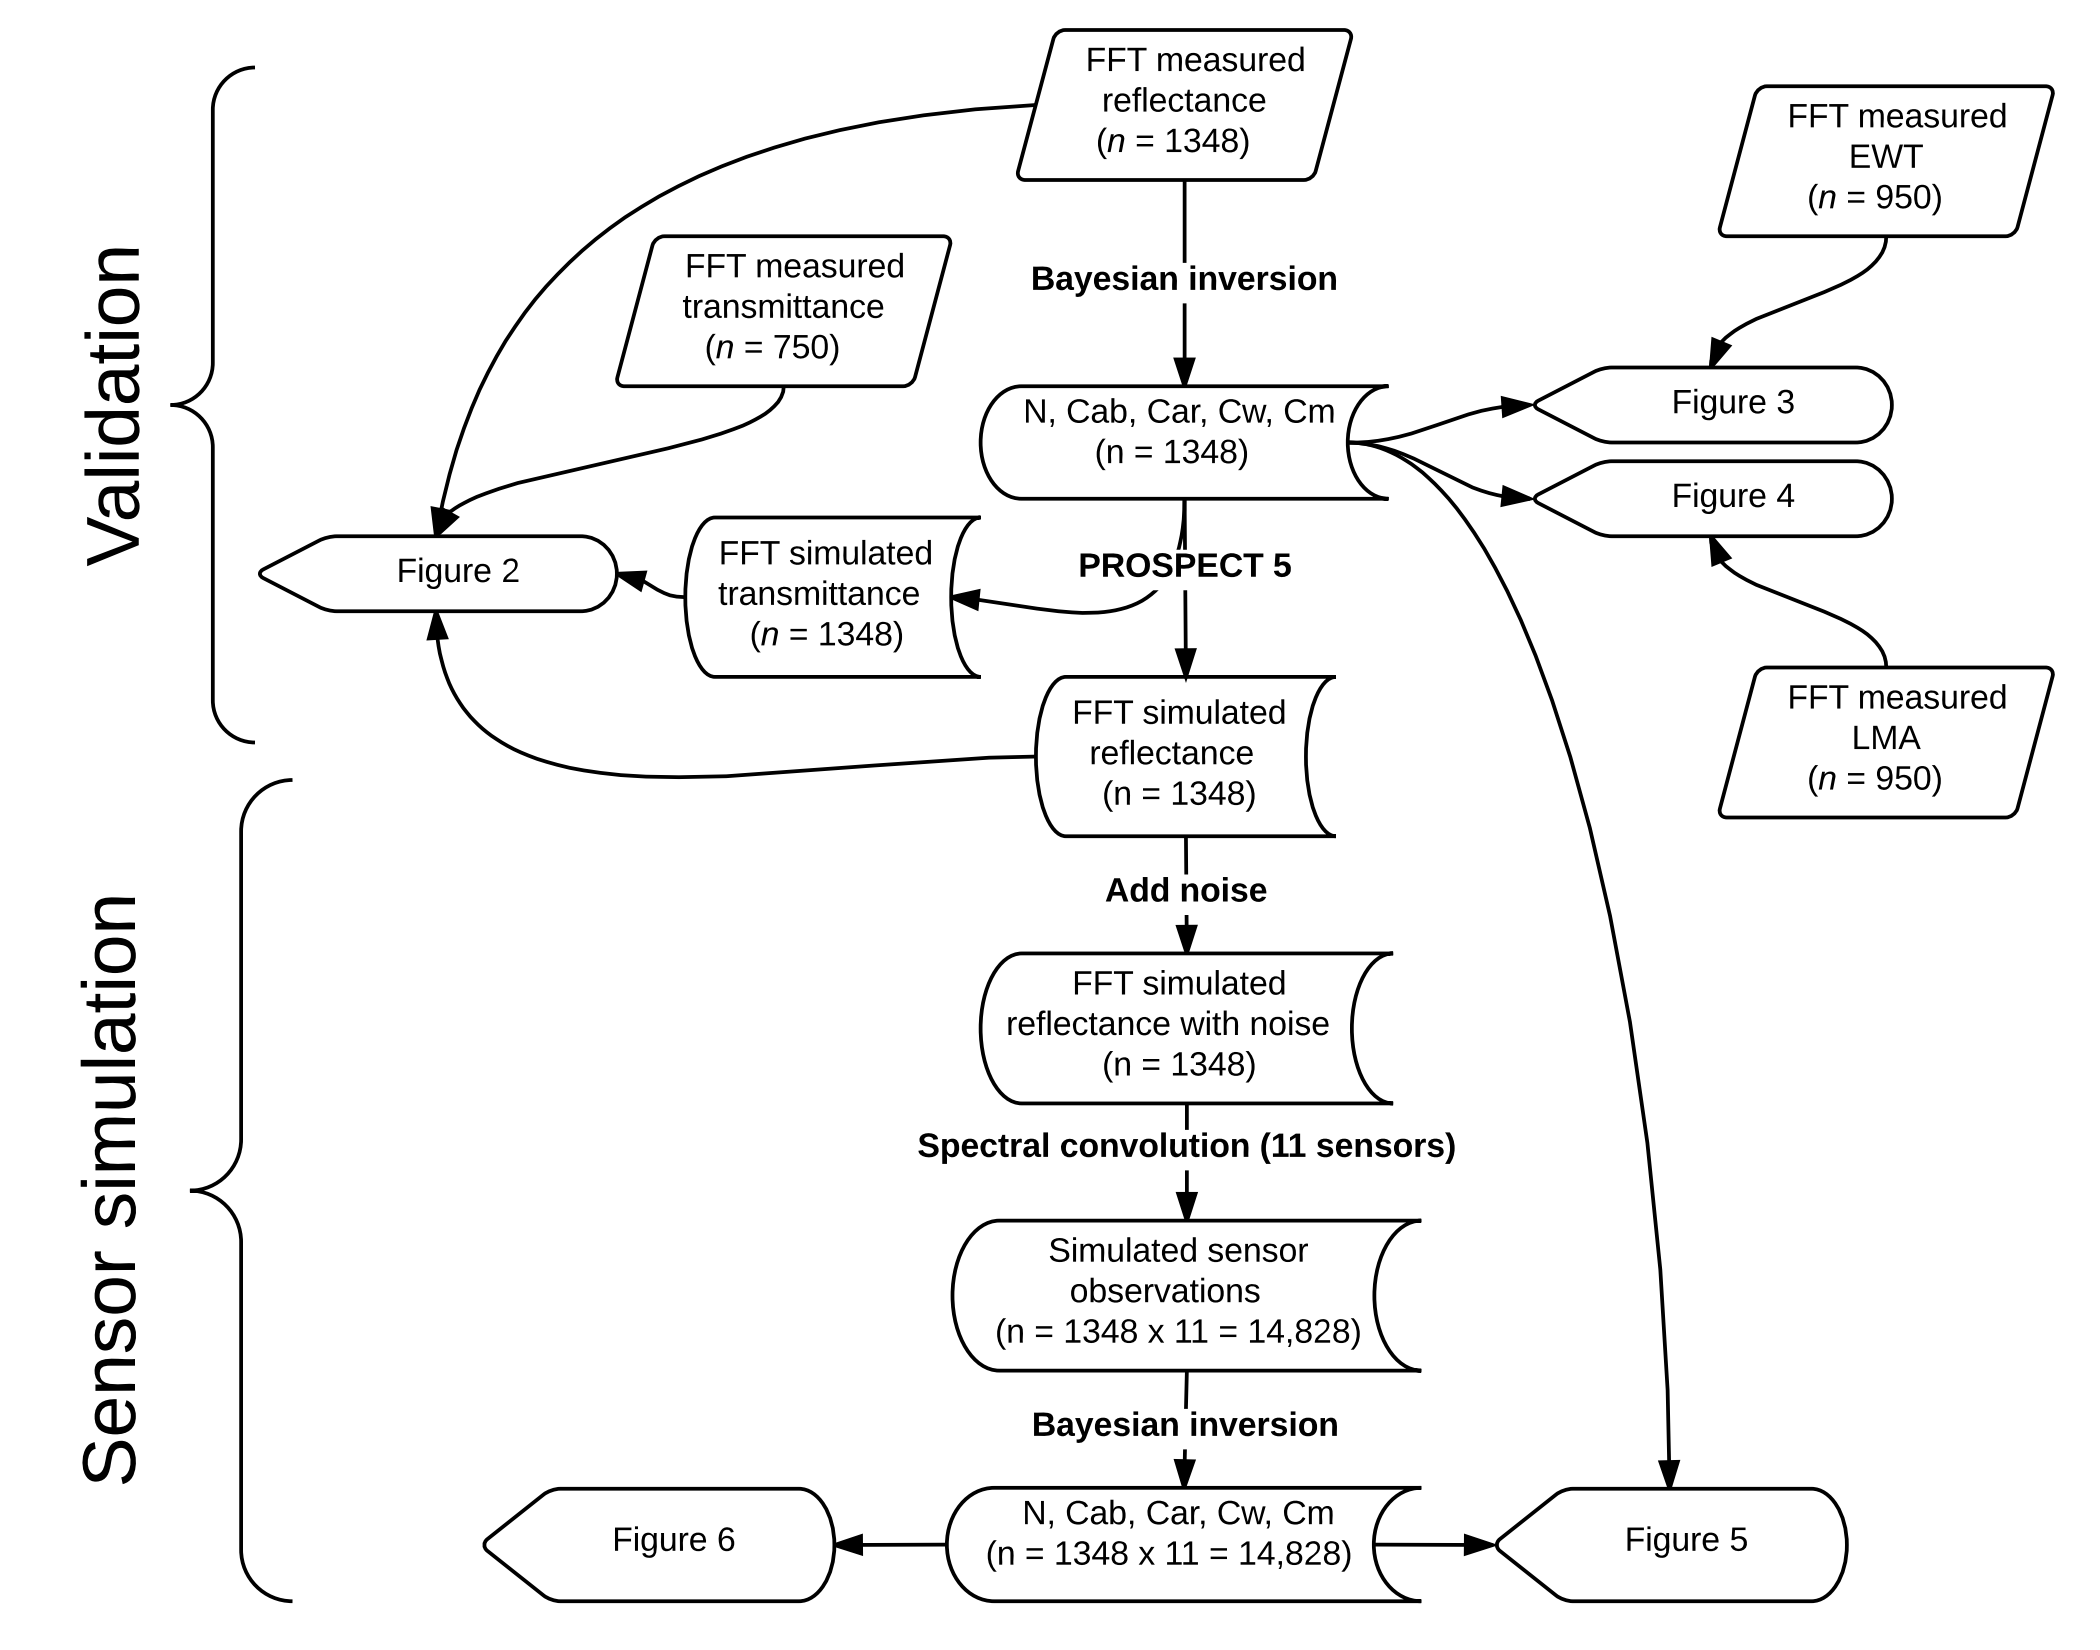
\includegraphics[width=\textwidth]{2_rtm_inversion/figures/workflow.png}
  \caption{%
    Workflow illustrating the steps in this study as well as the figures to which they correspond.
  }\label{fig:pecanrtm-workflow}
\end{figure}

\section{Results}\label{sec:pecanrtm-results}

\subsection{Validation}

\subsubsection{Reflectance and transmittance}

For the inversion of synthetic spectra, we found no statistically significant ($p < 0.05$) spectral bias at any wavelength (not shown).% (Figure S6). %TODO: Figure
As well, the observed differences between input and simulated output were one to two orders of magnitude smaller than corresponding errors in the inversion of measured spectra (Figure~\ref{fig:pecanrtm-specvalidation}).%, Figure S6). %TODO: Figure references
These results collectively illustrate that our algorithm is unbiased and contributes minimally to errors in the inversion of measured spectra.

For the inversion of measured spectra, we observed substantial variability in the spectral bias across all analyzed leaves, resulting in statistically significant ($p < 0.05$) bias in only a few specific wavelength regions (Figure~\ref{fig:pecanrtm-specvalidation}). % TODO: Figure ref
For both broadleaf and needle-leaf conifer species, reflectance was typically overestimated between 1600 and 1900 nm and underestimated between 1000 and 1300 nm and between 2000 and 2500 nm.
The errors in the 1600 to 1900 nm and 2000 to 2500 nm ranges covered more wavelengths and had larger magnitude for conifer species than broadleaved species.
Broadleaved species also had a statistically significant reflectance overestimate in the 400 to 500 nm range and an underestimate at 1300 nm, while conifer species had a significant reflectance overestimate at 1300 nm.

For both measured and synthetic spectra, transmittance bias ($BIAS = -0.0133$) was, on average, greater in magnitude than reflectance bias ($BIAS = 0.0018$), with a mean positive bias for broadleaved species ($BIAS = 0.0012$) and a mean negative bias for conifer species ($BIAS = -0.0346$) (Figure~\ref{fig:pecanrtm-specvalidation}, Table~\ref{tab:pecanrtm-specerr}).
However, the between-leaf variability in bias was also large and resulted in statistically significant bias in only a small number of specific spectral regions.
For both broadleaved and conifer species, we observed a significant underestimate in transmittance in the chlorophyll a absorption 400 and 500 nm.
Specifically for conifer species, we also observed underestimates in transmittance at the vegetation ``red edge'' around 700 nm and at a water absorption feature around 1900 nm.

\begin{figure}
  \centering
  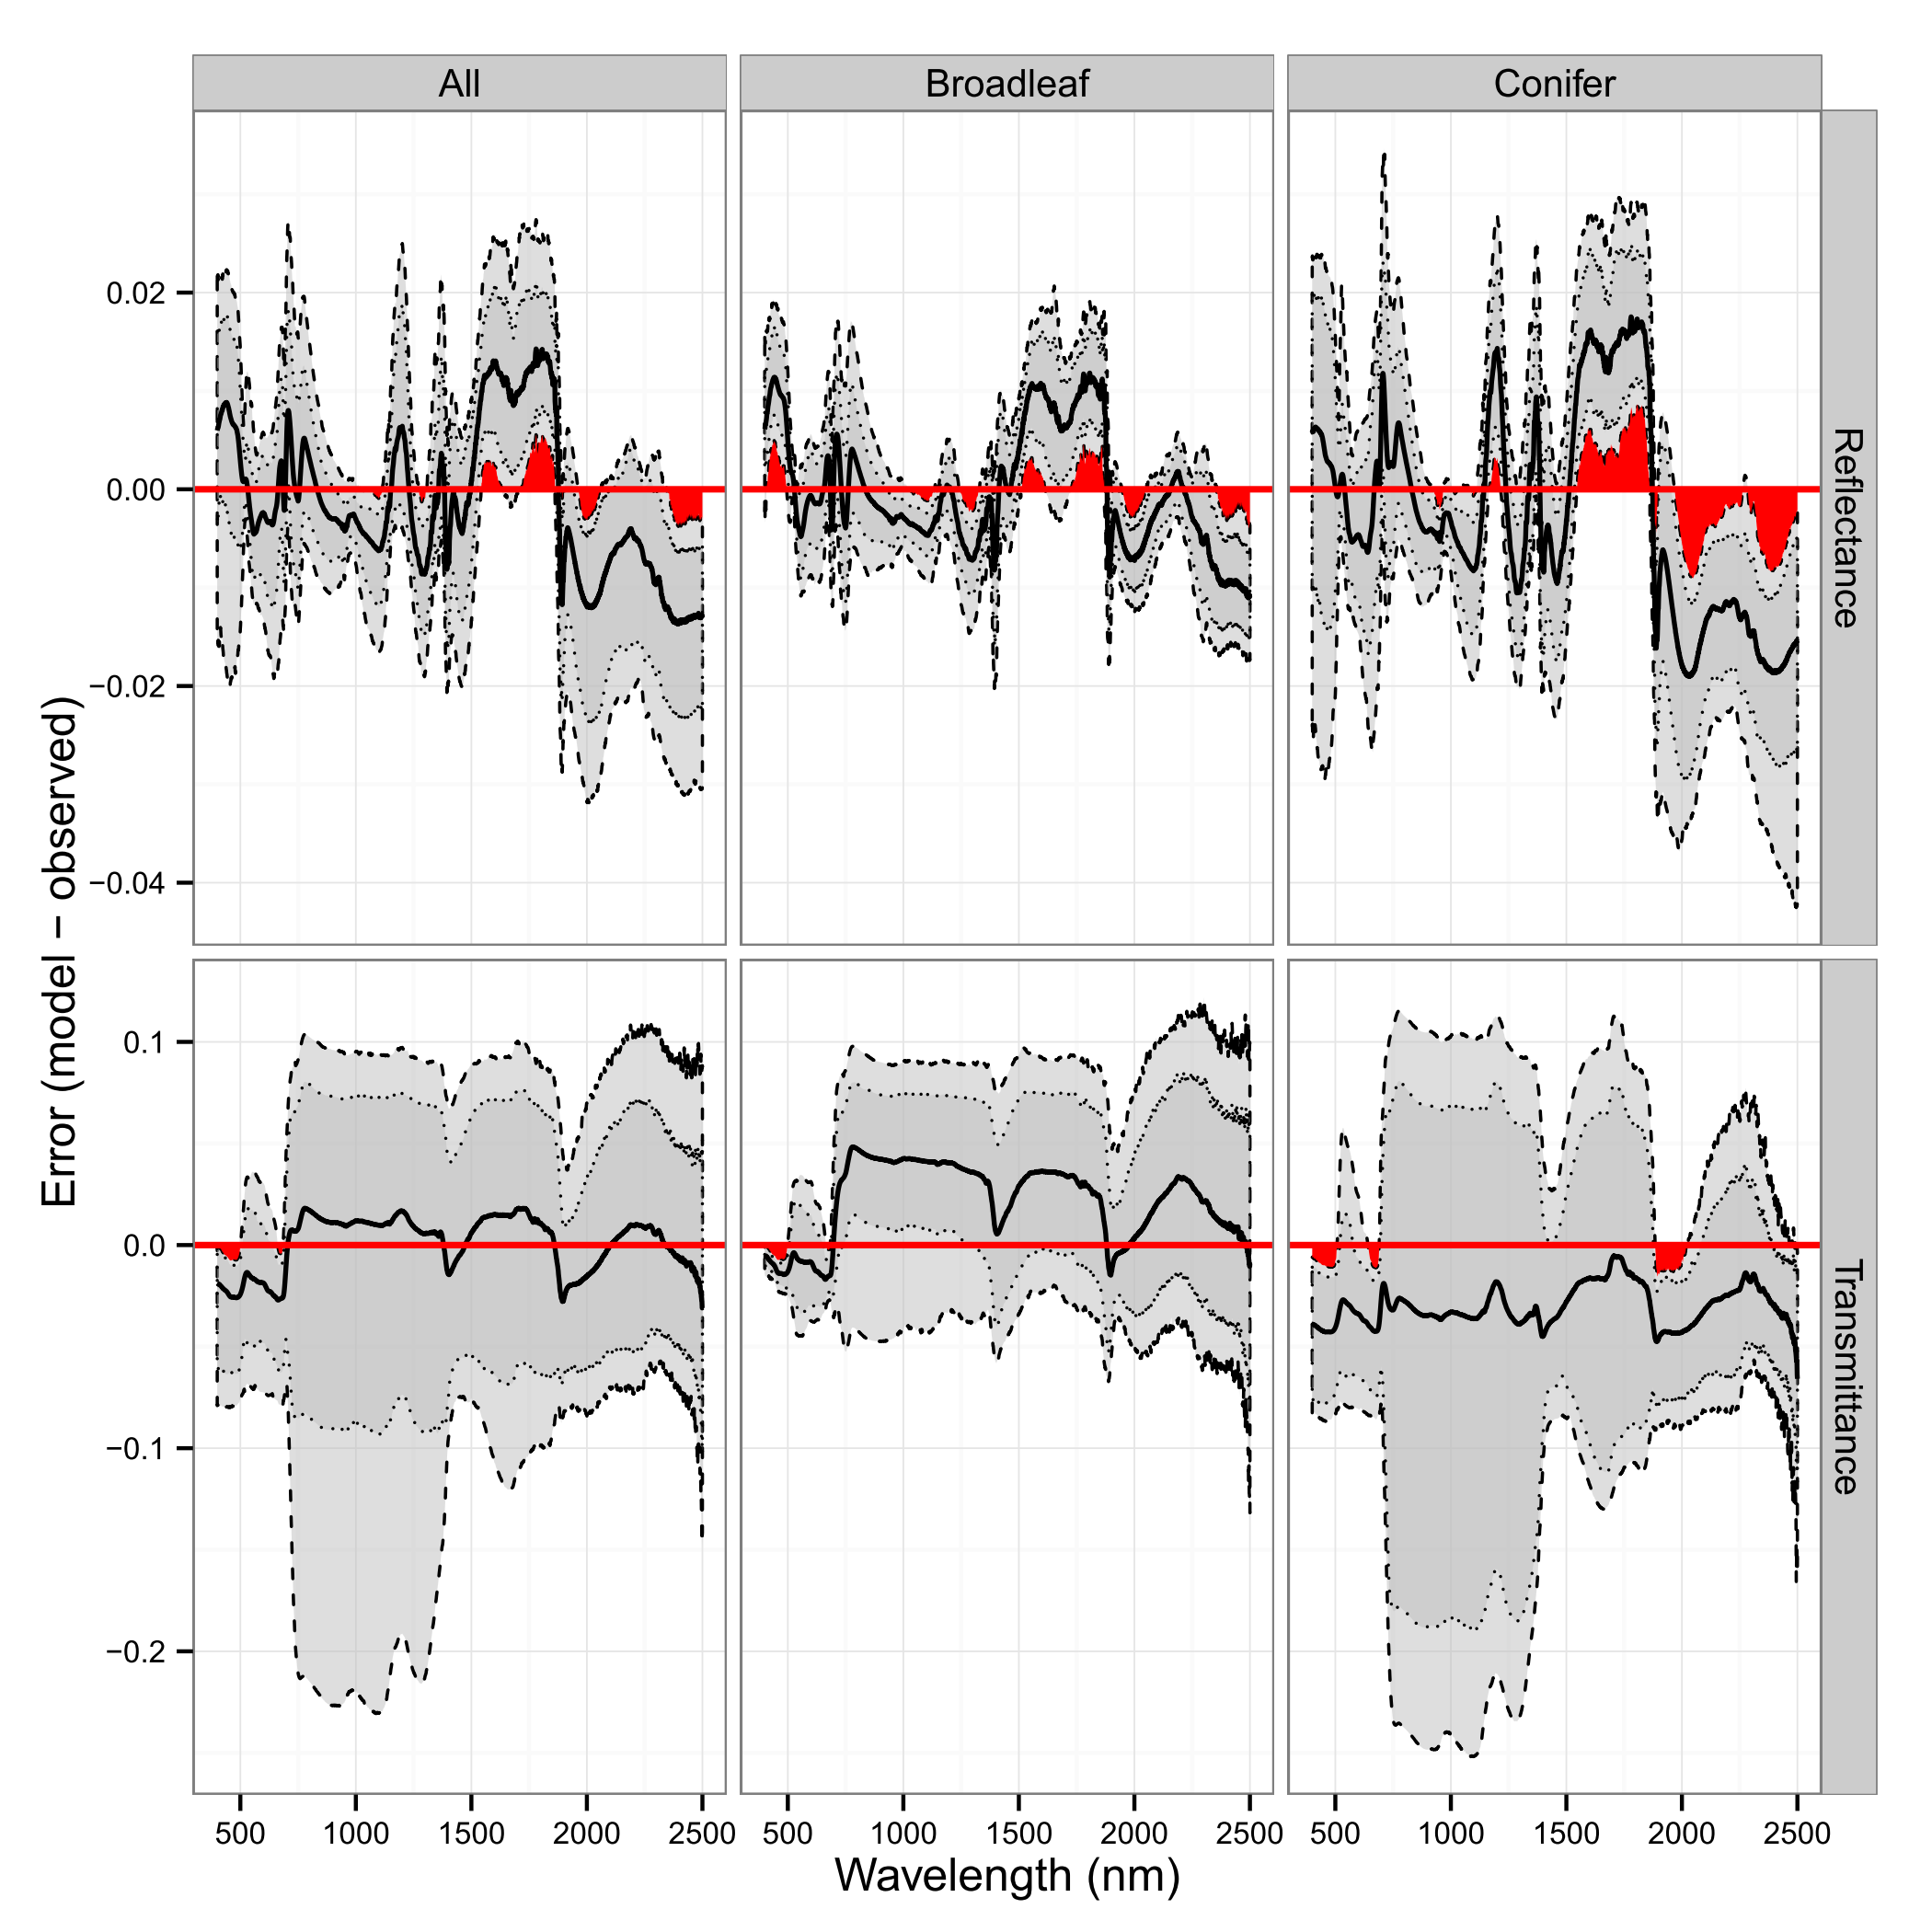
\includegraphics[width=\textwidth]{2_rtm_inversion/figures/spec_validation.png}
  \caption{%
    Bias in FFT simulated reflectance (top) and transmittance (bottom) spectra compared to measurements over all leaves (left) and only hardwood (middle) and conifer (right) species. 
    For a given wavelength,
    the solid black line is the mean bias,
    the dark grey bounded by the dotted line is the 90\% confidence interval,
    the light grey region bounded by the dashed line is the 95\% confidence interval,
    the red line highlights a bias of 0,
    and the red shaded regions highlight bias significant at the 95\% confidence level.
  }\label{fig:pecanrtm-specvalidation}
\end{figure}

\begin{table}
  \centering
  \caption{%
    Reflectance (Refl.) and transmittance (Tran.) spectral validation error statistics aggregated across the visible (400--800 nm) and infrared (801--2500 nm) regions.
    Values from other studies are included for comparison.
  }\label{tab:pecanrtm-specerr}
  \resizebox{\textwidth}{!}{%
    \begin{tabular}{clcccccc}
      \toprule
      & & \multicolumn{3}{c}{Visible} & \multicolumn{3}{c}{Infrared}\\
      & & RMSE & BIAS & SEPC & RMSE & BIAS & SEPC \\
      \midrule
      \multirow{7}{*}{Refl.} & FFT All & 0.0083 & 0.0018 & 0.0071 & 0.0098 & -0.0020 & 0.0061 \\
                             & --- Broadleaf & 0.0063 & 0.0023 & 0.0042 & 0.0064 & -0.0009 & 0.0034 \\
                             & --- Conifer & 0.0101 & 0.0011 & 0.0090 & 0.0127 & -0.0035 & 0.0064 \\
                             & Feret et al.~(2008): CALMIT & 0.032 & 0.010 & 0.028 & --- & --- & --- \\
                             & --- ANGERS & 0.019 & 0.001 & 0.019 & 0.016 & 0.003 & 0.014 \\
                             & --- HAWAII & 0.021 & -0.008 & 0.020 & 0.036 & -0.031 \\
                             & Di Vittorio (2009) & 0.0255 & 0.005 & --- & --- & --- & --- \\
      \midrule
      \multirow{7}{*}{Trans.} & FFT All & 0.0404 & -0.0133 & 0.0336 & 0.0551 & 0.0040 & 0.0537 \\
                              & --- Broadleaf & 0.0248 & 0.0012 & 0.0167 & 0.0450 & 0.0266 & 0.0336 \\
                              & --- Conifer & 0.0553 & -0.0346 & 0.0389 & 0.0661 & -0.0293 & 0.0566 \\
                              & Feret et al.~(2008): CALMIT & 0.029 & -0.005 & 0.025 & --- & --- & --- \\
                              & --- ANGERS & 0.018 & -0.005 & 0.017 & 0.016 & 0.001 & 0.015 \\
                              & --- HAWAII & 0.022 & 0.003 & 0.020 & 0.020 & -0.003 & 0.017 \\
                              & Di Vittorio (2009) & 0.0422 & 0.0294 & --- & --- & --- & --- \\
      \bottomrule
    \end{tabular}
  }
\end{table}

\begin{table}
  \centering
  \caption{%
    Error statistics for the comparison of inversion estimates of PROSPECT parameters Cw and Cm and measured values of equivalent water thickness (EWT) and leaf dry mass per unit area (LMA), respectively.
    Values from other inversion studies are included for comparison.
  }\label{tab:pecanrtm-paramerr}
  \begin{tabular}{p{2cm}lccccc}
    \toprule
    & & RMSE & BIAS & SEPC & CV & RMS\%E \\
    \midrule
    \multirow{7}{*}{\vtop{\hbox{Cw / EWT }\hbox{(g m$^{-2}$)}}}
    & FFT Broadleaf & 17 & 5 & 16 & 18.8 & 21.64 \\
    & --- Conifer & 187 & 90 & 164 & 52.3 & 67.29 \\
    & Feret et al.~(2008): LOPEX & 17 & -3 & 17 & 15.2 & --- \\
    & --- ANGERS & 20 & -1 & 20 & 17.1 & --- \\
    & Feret et al.~(2011): \#3 & 27 & --- & --- & --- & --- \\
    & Li \& Wang (2011) & 12 & 5 & --- & 20.10 & --- \\
    \midrule
    \multirow{7}{*}{\vtop{\hbox{Cm / LMA}\hbox{(g m$^{-2}$)}}}
    & FFT Broadleaf & 20 & -18 & 9 & 24.5 & 43.75 \\
    & --- Conifer & 121 & 35 & 116 & 61.6 & 65.51 \\
    & Feret et al.~(2008): LOPEX & 34 & 21 & 27 & 51.0 & --- \\
    & --- ANGERS & 26 & 1 & 26 & 49.8 & --- \\
    & Feret et al.~(2011): \#3 & 31 & --- & --- & --- & --- \\
    & Li \& Wang (2011) & 8 & -7 & --- & 13.75 & --- \\
    \bottomrule
  \end{tabular}
\end{table}

\subsubsection{Leaf water content and mass per area}

Similar to the results of the spectral validation,
the inversion estimates of Cw and Cm (compared to measured values of EWT and LMA, respectively) displayed higher accuracy for broadleaf ($CV_{Cw} = 18.8\%$, $CV_{Cm} = 24.5\%$) versus conifer species ($CV_{Cw} = 52.3\%$, $CV_{Cm} = 63.3\%$) (Table~\ref{tab:pecanrtm-paramerr}).
For the broadleaved species, our parameter estimates were within the range observed previously (Table~\ref{tab:pecanrtm-paramerr}).
While the inversion estimates for conifer species show a lower performance compared to broadleaf trees, the error inversion results were primarily driven by a single plant functional type—early successional conifers, which consisted entirely of pine species (\textit{Pinus} family).
Notably, a few estimates for mid-successional conifer species displayed significant divergence with observations, but in general fell along the 1:1 relationship (Figures~\ref{fig:pecanrtm-ewt} and~\ref{fig:pecanrtm-lma}).

\begin{figure}
  \centering
  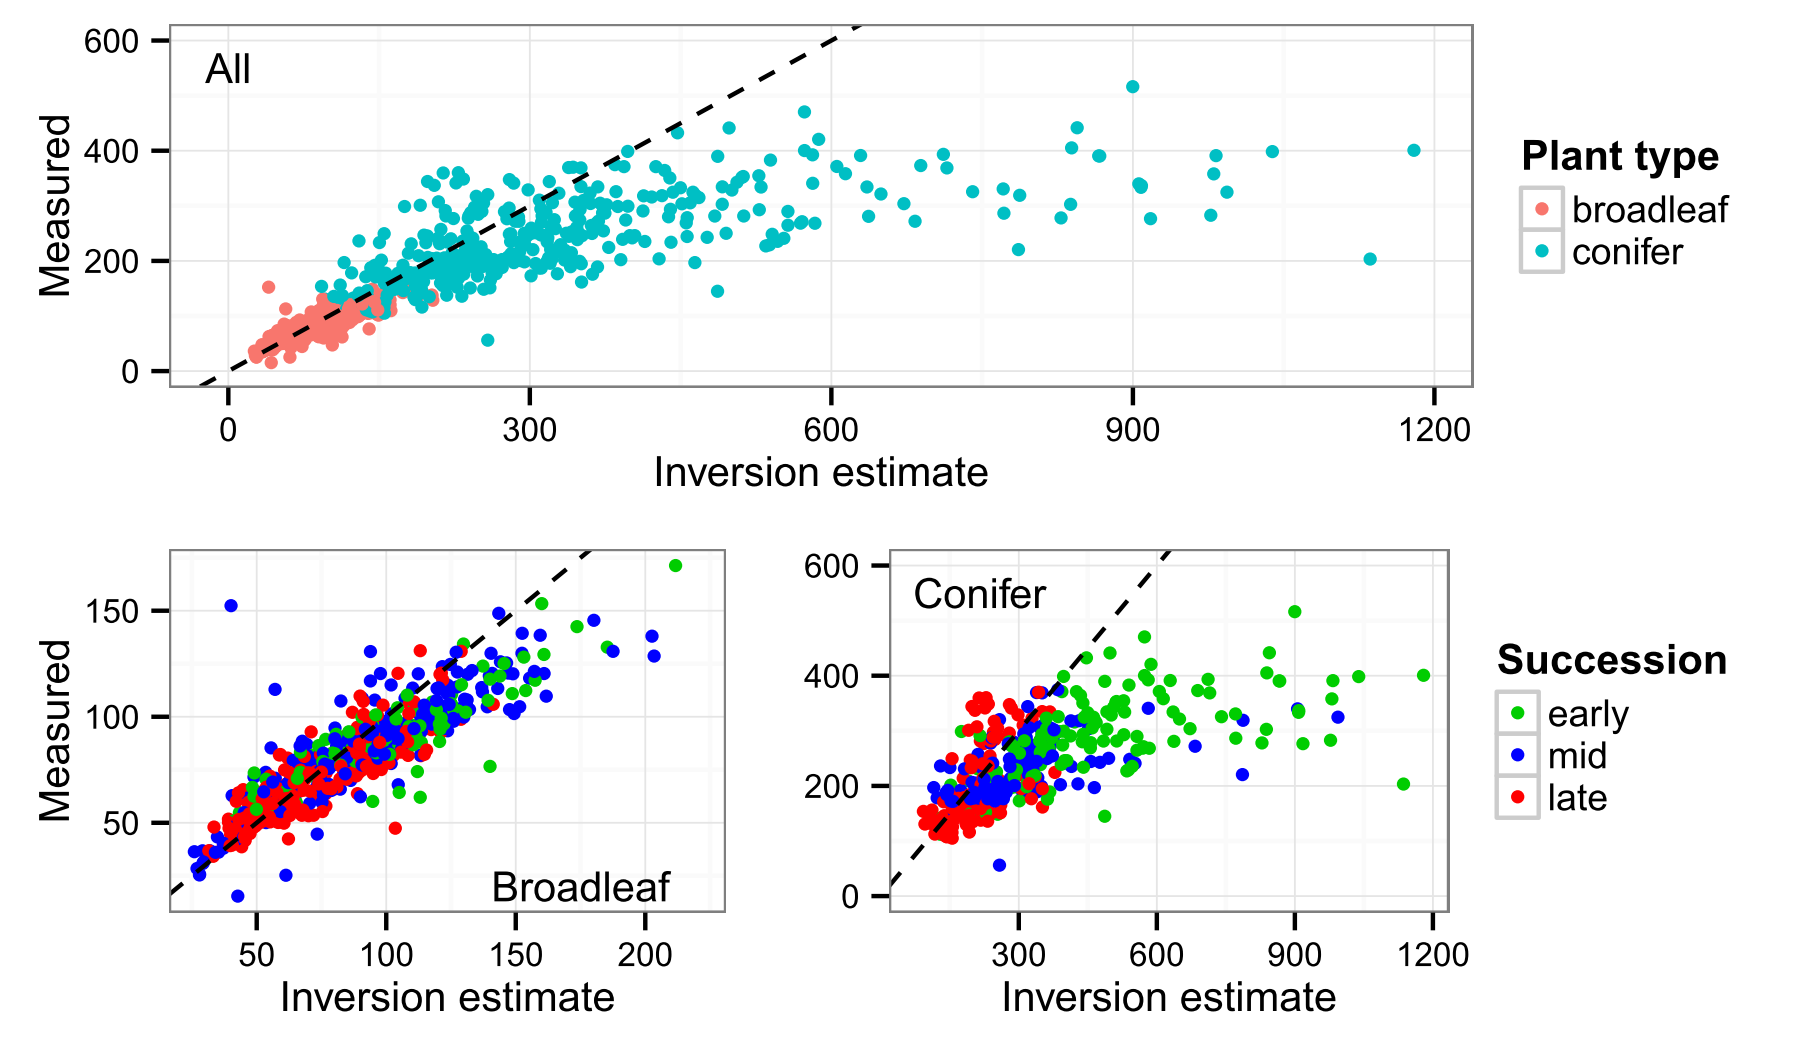
\includegraphics[width=\textwidth]{2_rtm_inversion/figures/ewt_validation.png}
  \caption{%
    Modeled and observed equivalent water thickness (g m$^{-2}$) for both conifers and hardwoods (top), just hardwoods (bottom left), and just conifers (bottom right).
    Point colors indicate plant type (top) or successional stage (bottom).
    The dashed line represents a 1:1 fit.
  }\label{fig:pecanrtm-ewt}
\end{figure}

\begin{figure}
  \centering
  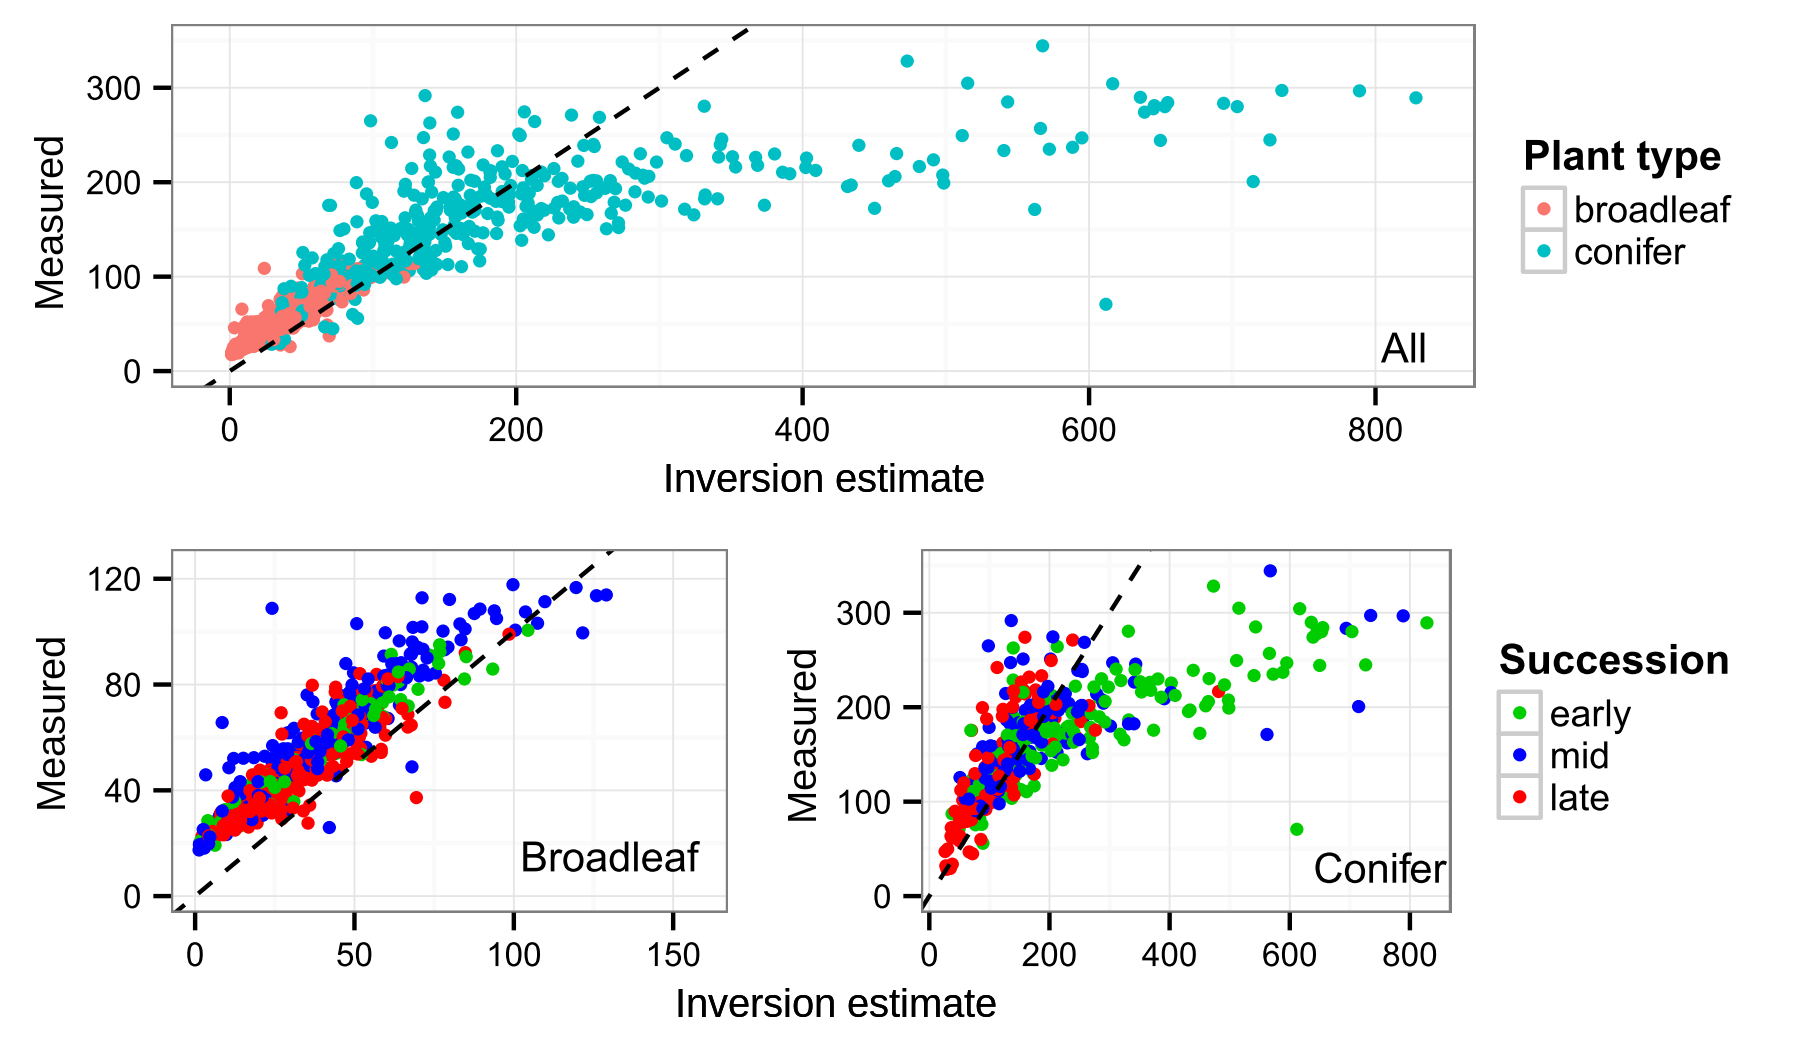
\includegraphics[width=\textwidth]{2_rtm_inversion/figures/lma_validation.png}
  \caption{%
    Modeled and observed leaf dry mass per unit area (g m$^{-2}$) for both conifers and hardwoods (top), just hardwoods (bottom left), and just conifers (bottom right).
    Point colors indicate plant type (top) or successional stage (bottom).
    The dashed line represents a 1:1 fit.
  }\label{fig:pecanrtm-lma}
\end{figure}

\subsection{Sensor simulation experiment}

\subsubsection{Parameter error}

\begin{table}
  \centering
  \caption{%
    Uncertainty and relative bias in parameter estimates from inversion of simulated spectra filtered through relative spectral response curves of different sensors.
  }\label{tab:pecanrtm-sensorerror}
  \resizebox{\textwidth}{!}{%
  \begin{tabular}{ccccccccccc}
    \toprule
    & \multicolumn{5}{c}{Uncertainty ($\pi$)} & \multicolumn{5}{c}{Relative bias ($\alpha$)} \\
    Sensor & N & Cab & Car & Cw & Cm & N & Cab & Car & Cw & Cm \\
    \midrule
    ASD Field Spec & 0.20 & 0.54 & 2.91 & 0.26 & 1.33 & -0.001 & 0.05 & 0.08 & 0.01 & -0.05 \\
    AVIRIS NG & 0.87 & 2.36 & 12.78 & 1.12 & 5.81 & -0.004 & 0.05 & -0.03 & 0.004 & -0.03 \\
    AVIRIS Classic & 1.62 & 4.61 & 26.06 & 2.13 & 11.02 & -0.04 & 0.06 & -0.44 & -0.01 & -0.08 \\
    Hyperion & 1.69 & 4.81 & 27.35 & 2.23 & 11.44 & -0.04 & 0.05 & -0.49 & -0.02 & -0.06 \\
    CHRIS-Proba & 21.93 & 20.77 & 53.86 & 106.5 & 173.8 & -0.71 & -0.50 & -2.52 & 2.41 & 87.84 \\
    Landsat 5 & 8.90 & 17.14 & 114.8 & 13.32 & 66.43 & -1.53 & -0.64 & -5.16 & -0.76 & -0.89 \\
    Landsat 7 & 8.84 & 21.90 & 134.2 & 12.94 & 66.07 & -1.52 & 0.55 & -9.17 & -0.77 & -0.91 \\
    Landsat 8 & 4.31 & 12.23 & 118.5 & 11.05 & 27.99 & -0.33 & 0.28 & -3.02 & -0.32 & -0.005 \\
    MODIS & 10.29 & 15.99 & 220.5 & 16.65 & 86.00 & -1.20 & 0.07 & -29.14 & -1.88 & 5.43 \\
    VIIRS & 2.49 & 13.24 & 174.4 & 4.75 & 18.23 & -0.09 & 1.57 & -18.06 & -0.09 & 0.004 \\
    AVHRR & 25.47 & 114.2 & 263.3 & 74.58 & 179.1 & -0.26 & -7.47 & -39.04 & -8.04 & 77.21 \\
    \bottomrule
  \end{tabular}
  }
\end{table}

\begin{figure}
  \centering
  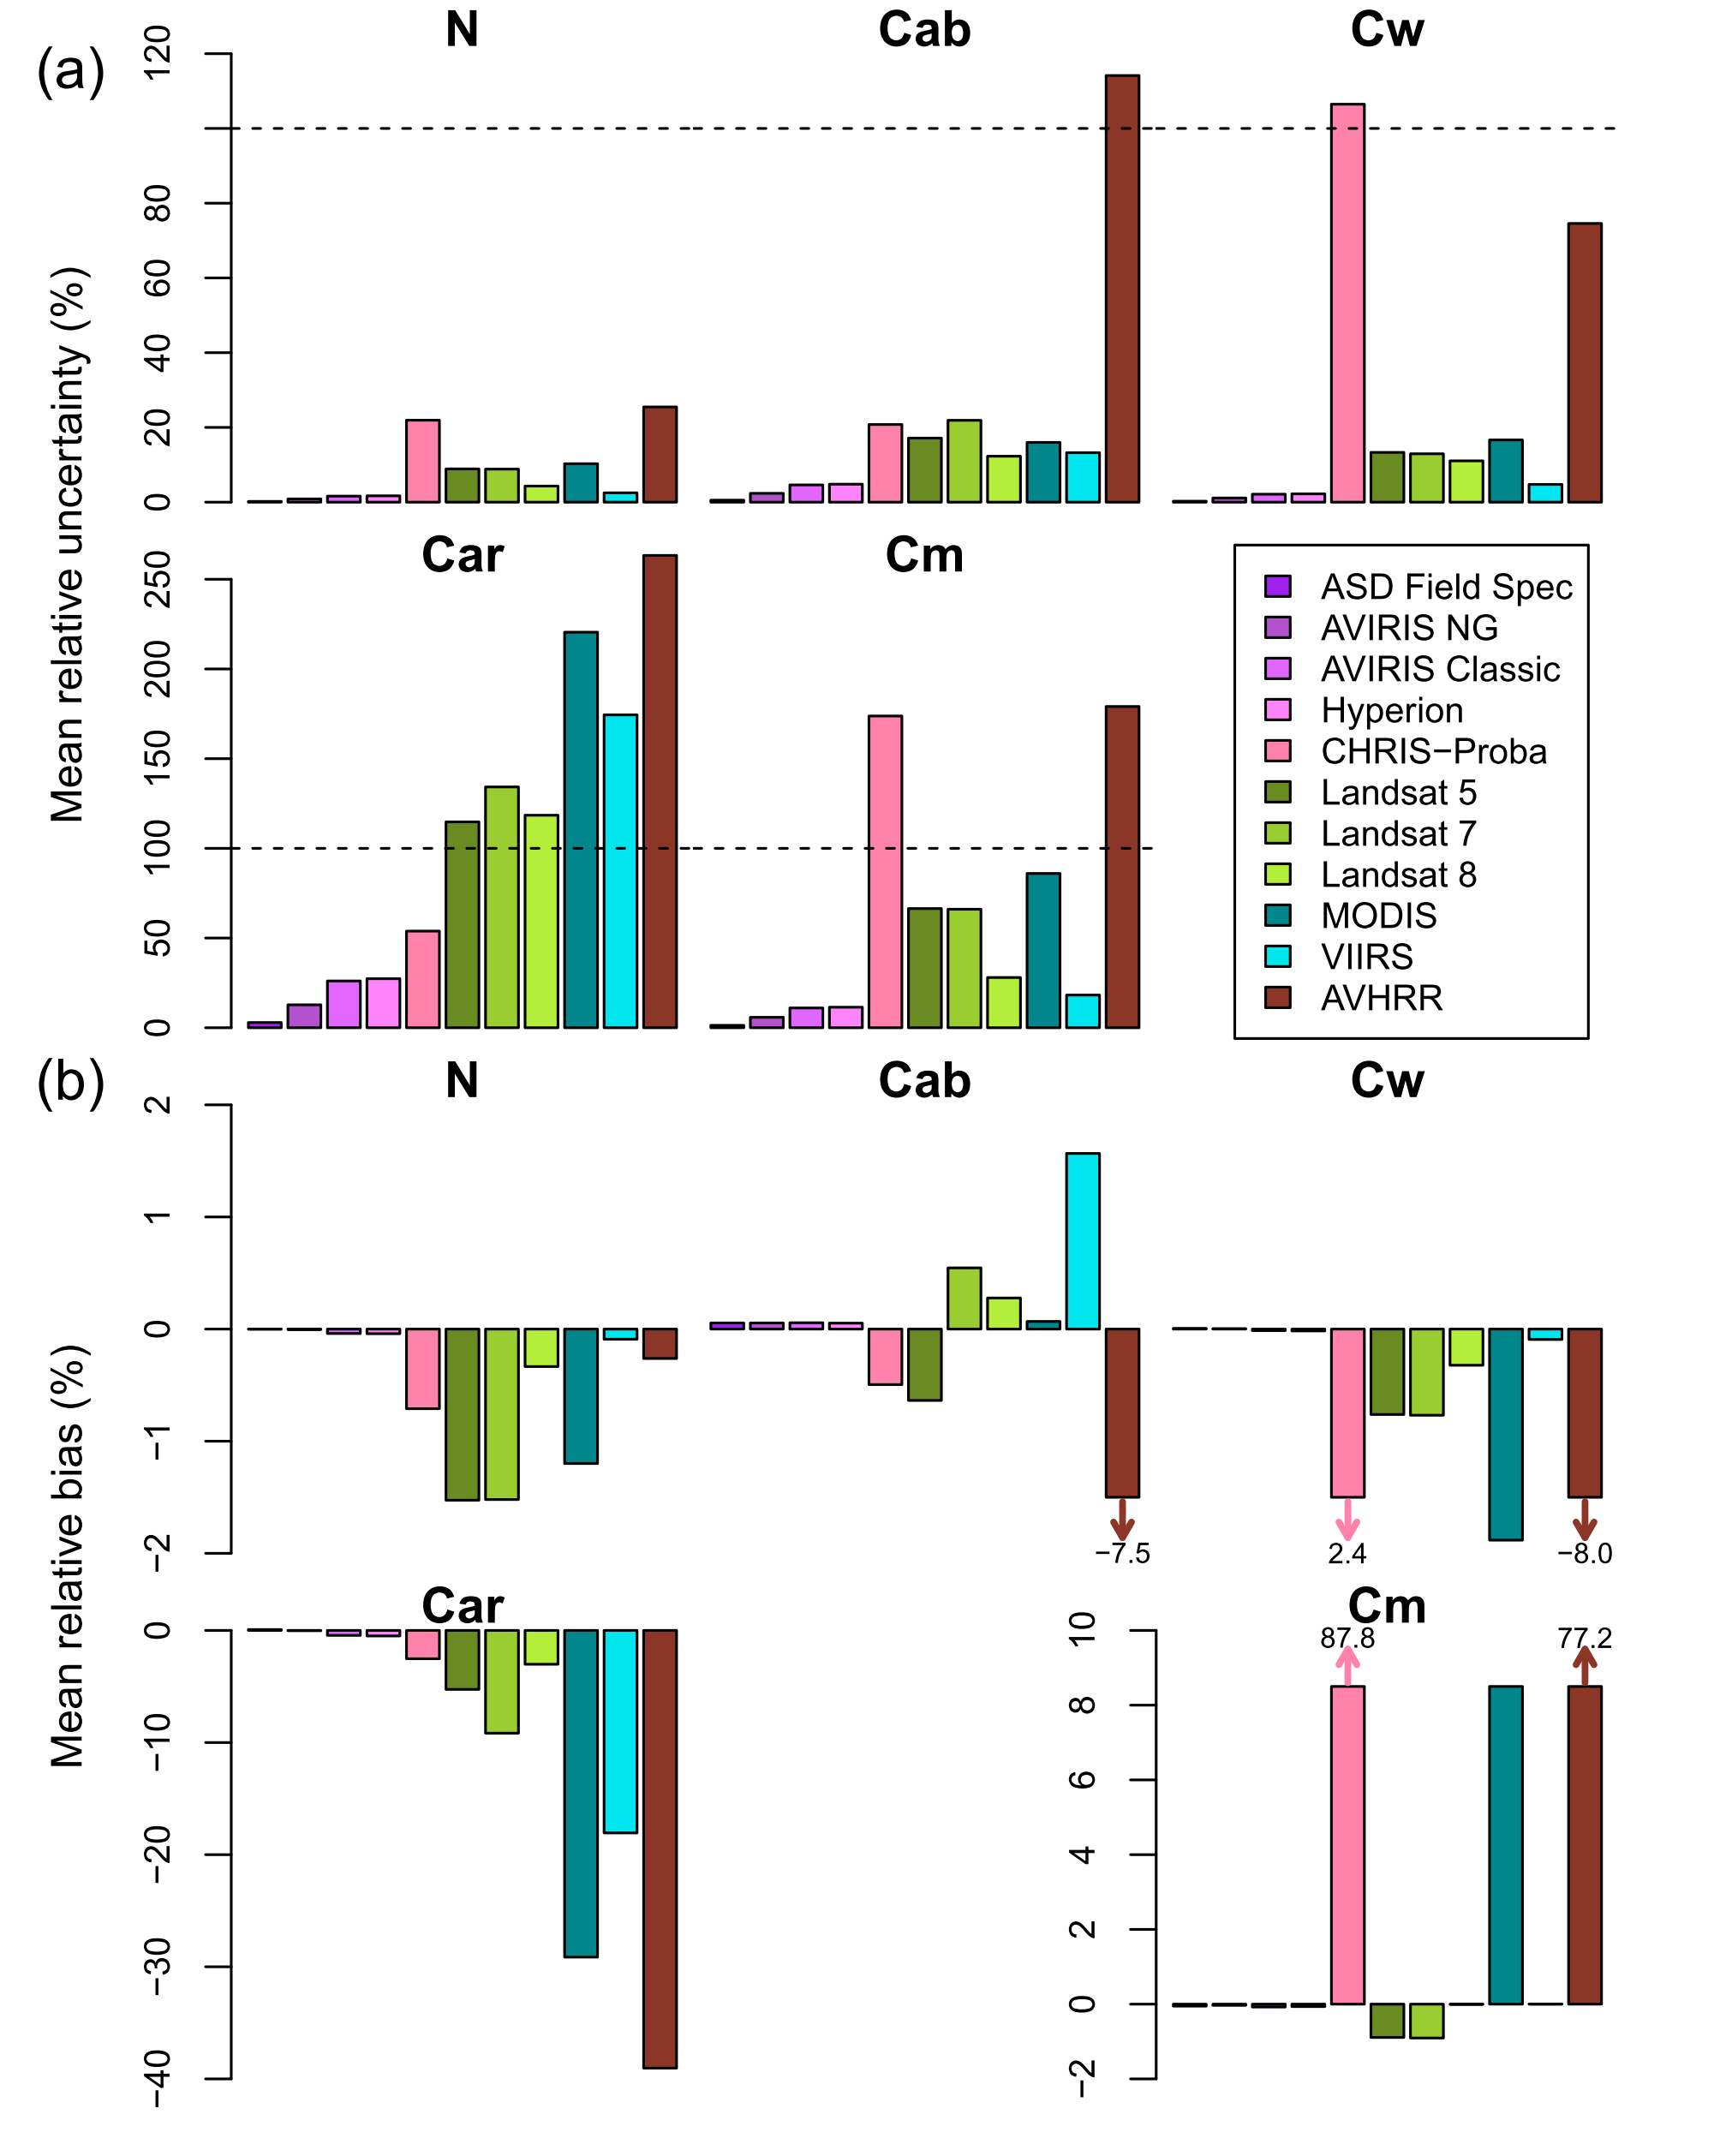
\includegraphics[width=\textwidth]{2_rtm_inversion/figures/mean_error.png}
  \caption{%
    Mean uncertainty (a) and relative bias (b) (as defined in section 2.3) of inversion estimates for each parameter and simulated sensor.
    Sensors are arranged along the x-axis in approximate order of increasing spectral resolution.
  }\label{fig:pecanrtm-sensorerror}
\end{figure}

Across all of the selected sensors, the highest PROSPECT 5 parameter inversion uncertainty and bias were observed for Car (Figure~\ref{fig:pecanrtm-sensorerror}, Table~\ref{tab:pecanrtm-sensorerror}).
This can readily be explained by the Car specific absorption feature, which is both extremely narrow and overlaps substantially with that of Cab (not shown).
On the other extreme, the most accurate and least uncertain retrieved parameter was N, which is related to the reflectivity of the leaf across the entire spectrum (Figure~\ref{fig:pecanrtm-sensorerror}, Table~\ref{tab:pecanrtm-sensorerror}).
Despite relatively narrow absorption features, most simulated sensors were able to retrieve Cab with reasonably good accuracy, which is not surprising given the long history of monitoring vegetation pigmentation using various platforms.
Similarly, all sensors except CHRIS-Proba and AVHRR retrieved Cw with low uncertainty and bias, reflecting the wide and strong absorption features of water in the NIR and SWIR (Figure~\ref{fig:pecanrtm-sensorerror}, Table~\ref{tab:pecanrtm-sensorerror}).
The failure of CHRIS-Proba to retrieve Cw can be attributed to its inability to measure in this spectral range.
The retrieval accuracy for Cm was much more sensor dependent, with good performance among the simulated hyperspectral sensors, VIIRS, and Landsat 8, followed by lower performance for simulated Landsat 5 and 7 and MODIS, and a poor result for the simulated Chris-PROBA and AVHRR data (Figure~\ref{fig:pecanrtm-sensorerror}, Table~\ref{fig:pecanrtm-sensorerror}).
Although the specific absorption feature for Cm is very wide, the sensitivity of reflectance to Cm values is much lower than for other parameters and almost the entire feature can be masked or confounded by Cw (Figure S1).
This suggests that Cm is very dependent on precise locations of certain bands and therefore explains the differences in the estimate accuracy of apparently similar sensors like Landsat 5, 7, and 8 (Table~\ref{tab:pecanrtm-sensors}).
More generally, the importance of precise band widths and locations is evidenced by the noticeably better performance of Landsat 8 compared to Landsat 5 and 7 for certain parameters (Figure~\ref{fig:pecanrtm-sensorerror}, Table~\ref{fig:pecanrtm-sensorerror}) despite the subtle differences in the sensors’ respective bandwidths (Table~\ref{tab:pecanrtm-sensors}).

\subsubsection{Parameter uncertainty and covariance}

\begin{figure}
  \centering
  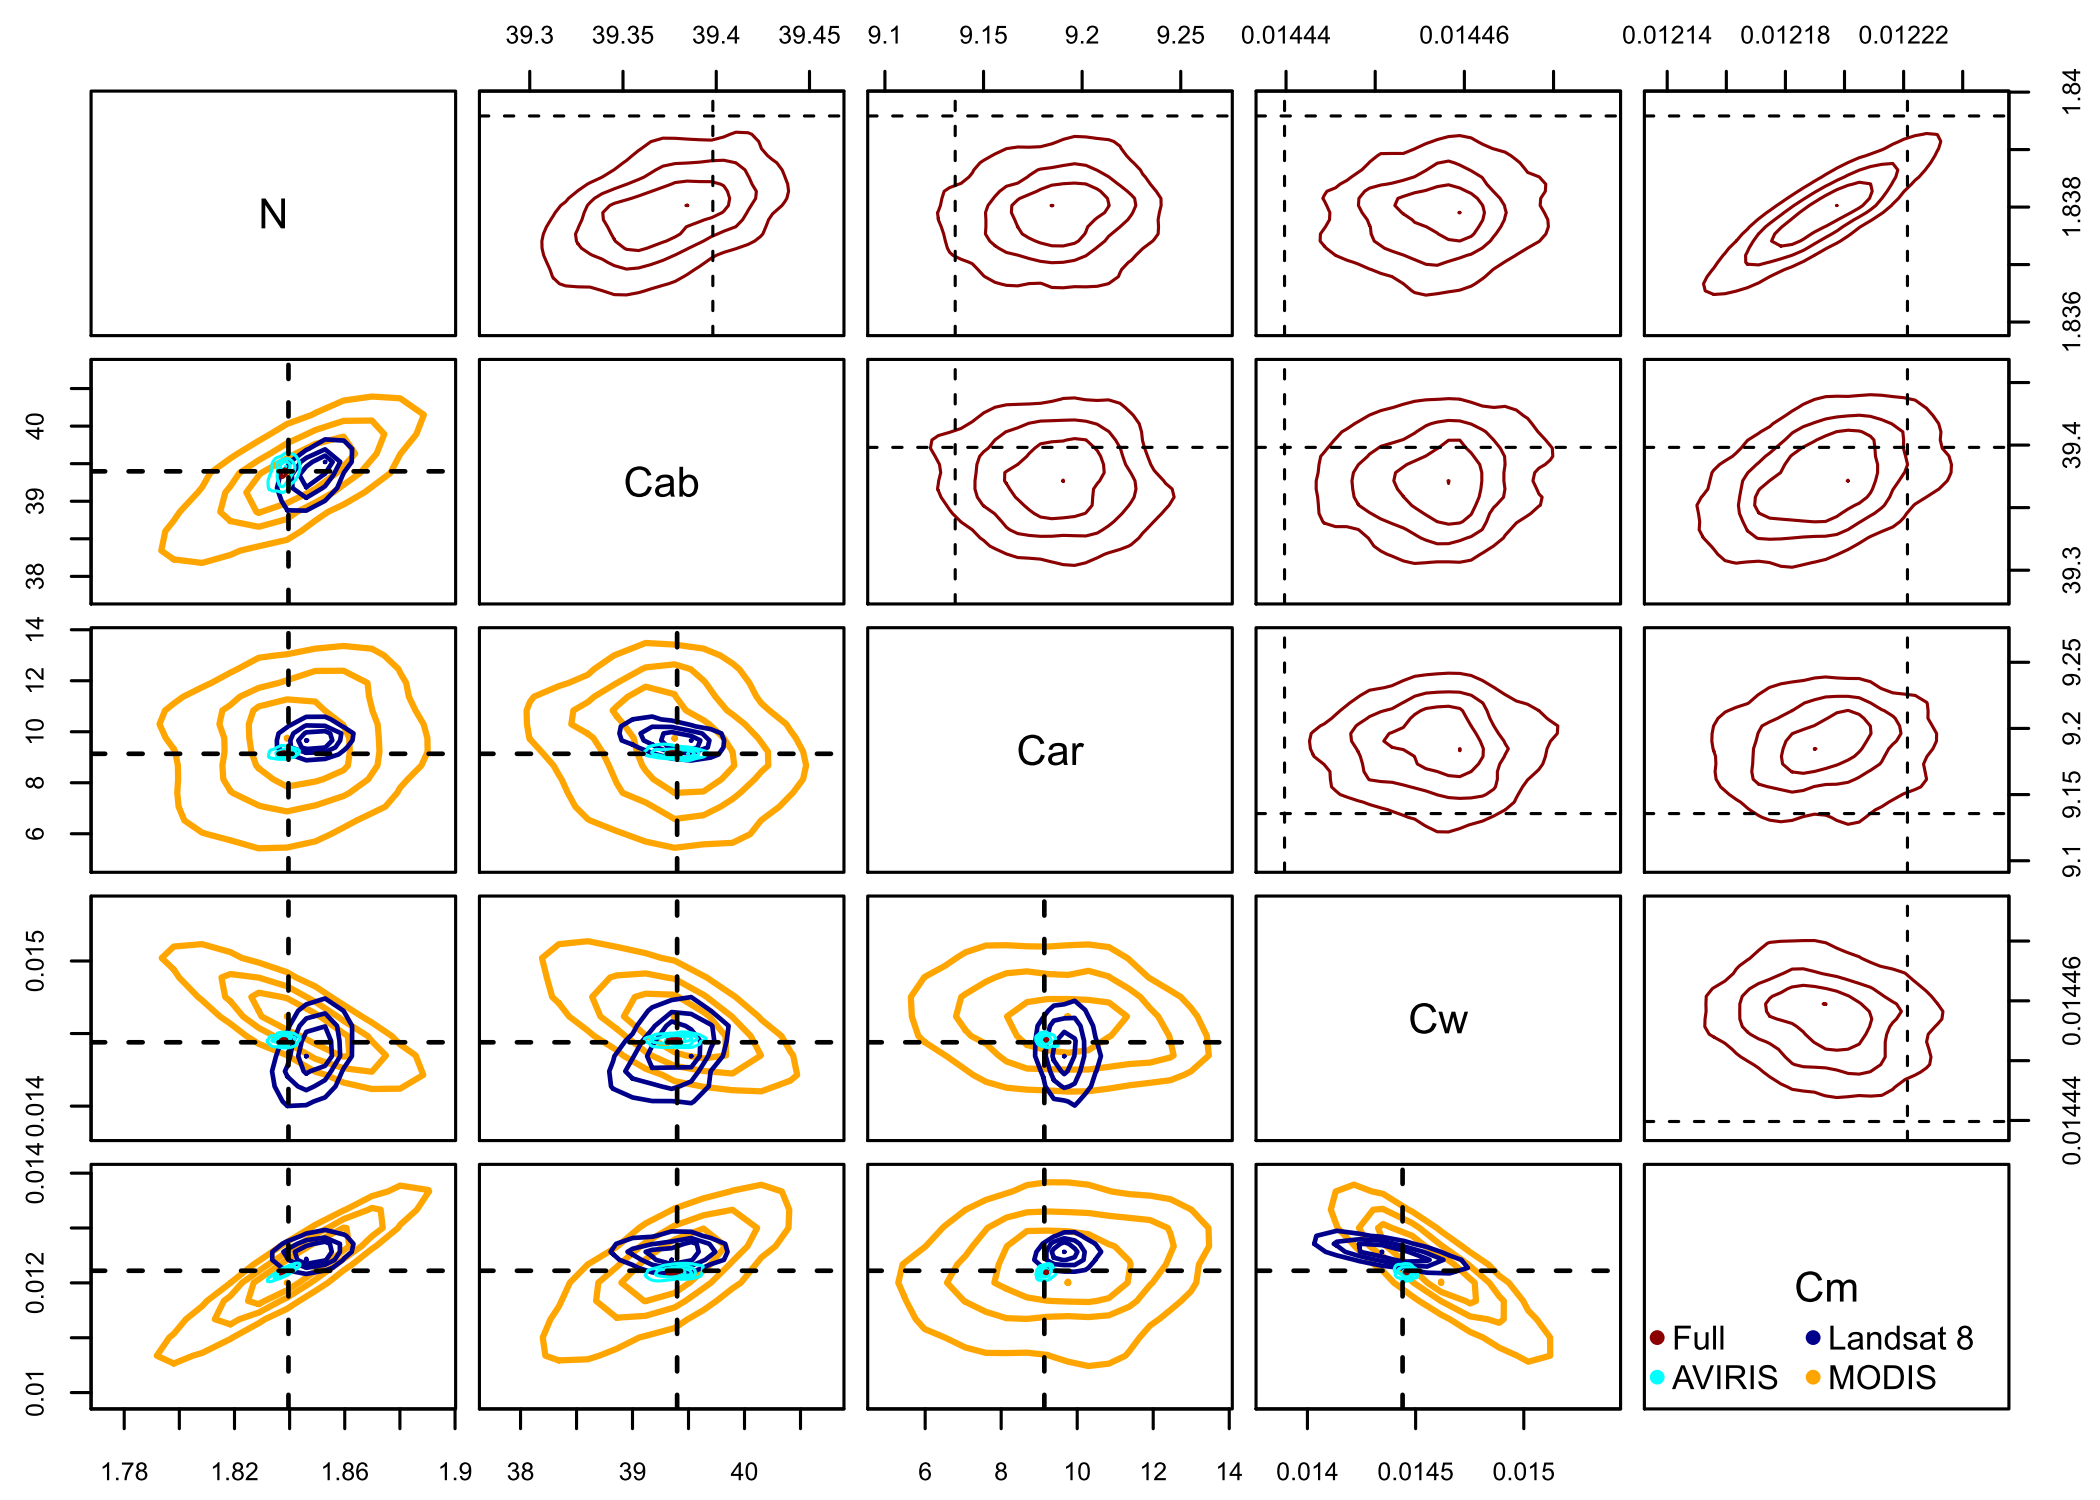
\includegraphics[width=\textwidth]{2_rtm_inversion/figures/joint_posterior.png}
  \caption{%
    Example joint probability distribution for parameter inversion estimates of simulated spectra using the full spectra (red; top panels) and the relative spectral response functions of AVIRIS NG (cyan), Landsat 8 (dark blue), and MODIS (orange). 
    Dotted lines indicate true parameter values. Note that the axis range of the top panels is substantially smaller than that of the bottom panels.
  }\label{fig:pecanrtm-jointpost}
\end{figure}

Figure~\ref{fig:pecanrtm-jointpost} shows an example of processed inversion output based on the high spectral resolution field spectrometer data and the spectral response functions of AVIRIS NG, Landsat 8, and MODIS\@.
All four plots are simulated from a single set of parameters, so differences in results are caused only by variations in spectral measurement characteristics.% (Figure S4). %TODO: Figure
Out of these four sensors, the uncertainties increase with approximately decreasing spectral resolution, with lowest uncertainties in the full spectra, second-lowest for AVIRIS NG, second highest for Landsat 8, and highest for MODIS\@.
The shapes of parameter covariances are distinctly different between these sensors, reflecting differences in the ability of the inversion to distinguish between parameters based on the available information.
Across all four sensors, we observe strong positive covariance between N and Cm, since these parameters influence wide regions of the reflectance spectrum in opposite ways.
Similarly, we also observe a positive covariance between N and Cab, although the strength of this covariance is not equal across sensors.
The remaining covariances are mostly specific to MODIS, whose band configuration increases the overlap between the associated parameters.

We find that inversion estimates for the field spectra are occasionally falsely overconfident.
For instance, the true value of N and Cw is outside the 95\% confidence limit of their estimated joint probability distribution at full, field spectrometer resolution.
That being said, this is less of an issue for the other sensors, where the joint probability distribution encompasses the true value.
This suggests that spectral resolution below 5 nm may not provide additional information content, particularly for the broad absorption features within leaves, because of the strong autocorrelation between adjacent wavelengths.
More importantly, although the joint posterior probability distributions from Landsat 8 and MODIS appear wide, the resulting parameter values are constrained by an order of magnitude or more compared to the priors.

\section{Discussion}\label{sec:pecanrtm-discussion}

In this manuscript, we reiterate the power of the Bayesian RTM inversion framework for using spectral data to characterize vegetation and monitor ecosystem dynamics.
The use of a physically-based model to describe the interaction of light with different vegetation structural and biochemical components improves the extent to which such an approach can be generalized across vegetation types and sub-orbital and spaceborne platforms compared to more empirical approaches.
Moreover, this physically-based approach enables estimation of vegetation properties from sensors of varying spectral resolution, and our ability to quantify uncertainty in our estimates provides the versatility to assess the performance of various sensors for a range of applications. 

Our inversion results are comparable to other studies~\cite{feret_2008_prospect,feret_2011_optimizing,li_2011_retrieval,divittorio_2009_enhancing}.
The results outperformed those of Feret et al.~(2011) despite the fact that we performed the inversion on measured spectra and inverted all five PROSPECT parameters,
whereas Feret et al.~(2011) performed inversions on synthetic spectra and did not attempt to estimate the structure parameter N. \nocite{feret_2011_optimizing}
As such, we suggest that our approach does not come at the cost of model performance, and, importantly, enables the use of a much wider range of spectral data to explore vegetation dynamics.
Our method contrasts with some previous methods~\cite[e.g., ]{feret_2008_prospect,feret_2011_optimizing} that utilize both reflectance and transmittance observations to invert leaf models such as PROSPECT\@.
These require the use of additional, expensive instruments, such as an integrating sphere, that typically introduce significant noise and potential errors in the measurements given their inadequate design across a range of leaf habits.
In addition, our approach suggests the possibility to instead use leaf reflectance observations alone to scale canopy-scale RTMs by coupling measured reflectance with simulated transmittance.

Placed in the context of past inversion studies, our work reveals some continuing challenges in the use of PROSPECT to model leaf optical properties and provides some guidance for future RTM development.
For instance, we noted issues with using PROSPECT to model reflectance and transmittance in the 400 to 500 nm range (Figure 2) that have also been reported in previous studies. %TODO: Figure reference
Feret et al.~(2008) observed a consistently negative transmittance bias and occasionally a positive or negative reflectance bias. \nocite{feret_2008_prospect}
Similarly, Croft et al.~(2013) report systematic underestimates of reflectance in this part of the spectrum. \nocite{croft_2013_modelling}
One possible source of bias is PROSPECT’s simplified description of leaf structure~\cite{jacquemoud_1990_prospect} and failure to account for specular reflectance off the leaf surface~\cite{grant_1987_diffuse}.
Another possible source of error is imprecise calibration of the leaf refractive index, which has a relatively strong wavelength dependence in the region of interest (400--500 nm)~\cite{feret_2008_prospect}.
Alternatively, this bias could be the result of the failure of the PROSPECT 5 model to properly represent the spectral properties of chlorophyll in leaves, potentially requiring additional calibration across a broader range of species and environments.
The common specific absorption feature for chlorophyll a and b ($kCab(\lambda)$) in PROSPECT 5 used in this study is empirically calibrated to a single data set~\cite[ANGERS; ]{feret_2008_prospect},
and many studies have shown that this feature may need to be re-calibrated to the data at hand to obtain accurate inversion estimates,
particularly for species dissimilar to those in the ANGERS data set~\cite{malenovsky_2006_applicability,moorthy_2008_estimating,zhang_2008_retrieving,li_2013_retrieval}.
As well, PROSPECT 5 fails to distinguish between chlorophyll a and b, which have overlapping but distinctly different absorption signatures and whose ratios have been shown to be affected by environmental conditions~\cite{blackburn_2006_hyperspectral,divittorio_2009_spectral,divittorio_2009_enhancing}.
Fortunately, it has been shown that not only can chlorophyll a and b be distinguished using imaging spectroscopy~\cite{divittorio_2009_pigment}, but that these differences can be incorporated into a RTM to improve its performance~\cite{divittorio_2009_enhancing}.

Reflectance in the SWIR region ($>1500 nm$)---where we observed significant reflectance bias (Figure 2)---is influenced by three PROSPECT parameters: N, Cw, and Cm (Figure S1). %TODO: Figure
All three parameters modulate reflectance in this spectral region monotonically: 
Reflectance increases with higher values of N and decreases with higher values of Cw and Cm (Figure S1). %TODO: Figure
This means that it is unlikely that incorrect parameter trade-off within the algorithm (e.g.\ preferentially selecting Cw over Cm) could contribute to this error.
Feret et al.~(2008) also reported similar reflectance bias patterns for the ANGERS data set despite using a different inversion methodology. \nocite{feret_2008_prospect}
We hypothesize this bias is the result of PROSPECT’s insufficient characterization of the specific absorption spectrum of leaf dry matter ($kCm(\lambda)$),
since the absorption characteristics of water ($kCw(\lambda)$) are well known and N is not dependent on an absorption feature.
This would also help explain the negative bias we observed between spectral inversion estimates of Cm and direct measurements of LMA (Figure 3, Table 3). %TODO: Figure ref
Other studies have also reported a bias but the direction of this bias has not been consistent, with some studies showing negative bias across all their data~\cite{li_2011_retrieval,cheng_2014_deriving} and others reporting a bias whose magnitude and direction is data-dependent~\cite{feret_2008_prospect}.
This may partially be explained by the simple treatment of non-pigment compounds in the current PROSPECT model, wherein protein, cellulose, hemicellulose, sugar, starch, and lignin are aggregated into a single parameter (Cm)~\cite{fourty_1996_leaf}.
As with chlorophyll, the absorption feature for Cm is empirically derived~\cite{feret_2008_prospect} and fails to represent variability in the relative abundance of the different components~\cite{poorter_causes_2009}.
Fortunately, Wang et al.~(2015) demonstrated that, with proper calibration, it is possible to use PROSPECT inversion to determine leaf protein as well as combined cellulose and lignin content. \nocite{wang_2015_applicability}
Furthermore, measurements of LMA are an aggregate of a number of constituents including chlorophyll, carotenoids, lipids, organic acids, phenolics, and vascular tissue~\cite{poorter_causes_2009}, which would positively bias the measurement compared to the spectral estimate.
Finally, it is possible that strong positive covariance between N and Cm (Figure 6) caused by their significant spectral overlap (Figure S1) interferes with accurate estimation of Cm. %TODO: Fig refs
However, based on our finding that inversions of simulated spectra did not display this problem (Field spectra in Figure 5; Figure S6), we conclude the error is in fact driven more by model formulation than by parameter identifiability. %TODO: Fig refs
We are aware of only one other study that attempted to estimate all five PROSPECT parameters (including the structure parameter, N) simultaneously: \nocite{li_2011_retrieval}
Li \& Wang (2011) presented a novel algorithm for PROSPECT inversion that assigns a separate merit function to each parameter (rather than a single common merit function for all parameters) and demonstrated its improved performance over traditional approaches.
However, although their new algorithm reduced error and bias in the LMA estimates, a negative bias comparable to the one we report still remained across all of their data sets. 

Based on these results, we suggest that future PROSPECT development should aim for finer distinction in leaf chemical components.
That being said, the introduction of additional parameters into a model must be approached with caution, as parameter precision and identifiability tend to decrease with model complexity.
The ability of our Bayesian inversion to quantify parameter uncertainty and covariance makes it useful for nested model selection.
An alternative approach to addressing the issue of empirically-calibrated absorption coefficients is to explicitly account for their uncertainty and covariance structures. 
Within our Bayesian framework, such uncertainties could be treated as observation errors and propagated to the uncertainty in parameter estimates.
In subsequent work, we will explore such a calibration using coupled spectral-trait data from multiple available datasets.

The relatively large magnitude in our observed transmittance bias (compared to reflectance) is likely the result of using only reflectance as input in our inversion.
A combined approach using measured reflectance and transmittance observations, collected on the same leaf samples, may have shown the variability distributed more evenly because the minimization of the residuals would have been more balanced between the two vectors of data.
Ultimately, higher uncertainties in transmittance estimates compared to reflectance are a consequence of the inherent challenges in using integrating spheres to measure transmittance, especially the substantial noise in the SWIR regions.
This is supported by the absence of significant systematic bias between measured and modeled transmittance across the overwhelming majority of the spectrum (Figure 2). %TODO: Fig ref
Moreover, although the confidence intervals on transmittance bias are as high as 25\% at some wavelengths, averaging over all spectra and aggregating across the visible (400 to 800 nm) and infrared (801 to 2500 nm) regions leads to results similar to those reported in other field spectra inversion studies, even though these studies used both reflectance and transmittance as input (Table S1). %TODO: Table ref
Although our overall transmittance RMSE values were two to three times higher than those reported by Feret et al.~(2008), \nocite{feret_2008_prospect}
these errors are inflated by the inclusion of conifer species, for which reflectance is harder to measure reliably and the assumptions of the PROSPECT model are not satisfied~\cite{jacquemoud_1990_prospect,divittorio_2009_enhancing,allen_1969_interaction}.
As well, measurements of needle-leaf transmittance often result in considerable noise in longer wavelengths (SWIR, >2000 nm) given
the physical challenges of making these measurements on needle-leaf species (and other leaf types),
generally poor lamp performance as compared to other methods,
and the much smaller transmission of light in these wavelengths (often resulting in signals below the precision of the instrument).
As such we would expect higher reported error compared to other leaf morphologies.
For example, in examining our broadleaf samples we observed that the statistics for transmittance are much closer to those reported by Feret et al.~(2008), despite not including measured transmittance in the inversion (Table S1). \nocite{feret_2008_prospect} %TODO: Table ref
Our transmittance error statistics are also similar to those reported for conifers by Di Vittorio (2009a) who used transmittance information and a re-calibrated version of the LIBERTY leaf RTM (Table 3). % TODO: Table ref, check Di Vittorio ref
Moreover, our reflectance statistics show error comparable to or lower than those reported in similar studies~\cite{feret_2008_prospect,divittorio_2009_enhancing}.

Through our sensor experiment, we explicitly demonstrate the tradeoffs between spectral information content and parameter uncertainty and identifiability.
With increasingly coarse spectral resolution, we observed not only wider parameter confidence intervals indicating higher uncertainty but also tighter covariance structures indicating a reduced ability to distinguish between parameters (Figure 6). %TODO: Figure ref
This comparison approach can be used to guide future enhancements of radiative transfer models by quantitatively showing whether a model of a given complexity is warranted given data of a particular quality.
For example, in our simulation experiment, all the full-range hyperspectral sensors were capable of accurately estimating chlorophyll and carotenoids, but the ability of multispectral sensors to do so was dramatically lower (Figures 5, S6, and S7; Table 5). %TODO: Figure ref
We therefore can conclude that the use of PROSPECT 5 is warranted when performing inversion of hyperspectral data, but PROSPECT 4 (which does not distinguish between pigments) may be preferable for multispectral data.
A similar framework can be used to determine the utility of increasingly complex future versions of PROSPECT that further differentiate leaf biochemical and structural components.

Importantly, the results of our sensor simulation experiment are highly idealized due to their failure to consider canopy structure, atmospheric effects, sun-sensor geometry, and sensor radiometric and spatial characteristics.
However, a similar Bayesian inversion framework has been shown to work on MODIS data for the related coupled leaf-canopy RTM PROSAIL~\cite{zhang_2005_estimating,zhang_2006_characterization,zhang_2009_satellite,zhang_2012_estimating} and we believe the framework can be readily applied to other RTMs that address many of the limitations of our study.
In future work, we will explore Bayesian spectral inversion of the coupled leaf-canopy RTM responsible for energy balance calculations in the ED2 ecosystem model~\cite{medvigy_2009_mechanistic} on atmospherically corrected and orthorectified AVIRIS imagery,
which will be an important milestone in bringing together the remote sensing and ecological modeling communities.
In the long run, our framework could also be extended to the inversion of coupled canopy-atmosphere models using a combination of meteorological and spectral data from Earth Observation satellites,
leveraging the relative advantages of each platform to generate unified time series of ecologically meaningful parameters with unprecedented spatial and temporal resolution.

\section{Conclusions}\label{sec:pecanrtm-conclusions}

This study introduces a novel application of Bayesian spectral inversion to the PROSPECT 5 leaf RTM that explicitly takes into account uncertainty and correlation in parameter estimates.
Validation of our algorithm on a coupled leaf spectral-trait database revealed accuracy comparable to previous inversion algorithms despite only using reflectance observations and the default PROSPECT model (i.e.\ no additional refinement of the specific absorption features).
By simulating reflectance measurements with the spectral characteristics of different remote sensing platforms, we were able to quantify the relationship between spectral resolution and parameter uncertainty.
Although our simulated observations are highly idealized, we believe the resulting patterns in retrieved parameter accuracy and precision are representative of the advantages and limitations of the spectral configurations of different sensors for remote sensing of vegetation.
Our work reinforces the notion that Bayesian spectral inversion provides a powerful and versatile framework for future RTM development and single- and multi-instrumental remote sensing of vegetation, and we encourage members of the remote sensing community to apply and build upon the tools we have developed.


\cleardoublepage

\chapter{Leaf optical properties shed light on foliar trait variability at individual to global scales}
\thispagestyle{myheadings}

\graphicspath{{3_prospect/}} 

\begin{abstract}

ABSTRACT GOES HERE

\end{abstract}

\section{Introduction}

A key objective of present-day ecosystem ecology is to develop a predictive understanding of how terrestrial ecosystems will respond to rapid and widespread enviromental changes defining the Anthropocene. 
Plant functional traits serve as bellwethers of many aspects of plant ecophysiology, and understanding how traits respond to biotic and abiotic forcings has become a top priority in terrestrial ecology.
As I discussed in Chapter 1, global trait databases are useful for evaluating theories about plant ecological strategies and can be used to constrain parameters of dynamic vegetation models.

However, there are fundamental limits on the sorts of ecological questions that can be answered using static trait databases.
For one, such databases are spatially and phylogenetically incomplete, often in domains most critical to the global climate system such as boreal and tropical forests~\cite{jetz2016_diversity}.
More importantly, because these databases generally do not contain observations collected on the same individuals through time, they are limited in their ability to inform us about direct dynamic responses of plant function to environmental changes.
These changes are perhaps most pronounced in deciduous plants, whose leaves within a single season undergo a full life cycle accompanied by dramatic changes in pigment concentrations~\cite{yang_2016_seasonal}, morphology~\cite{poorter_causes_2009}, and productivity~\cite{parent_2010_modelling}.
Such intra-specific and intra-individual changes also occur in evergreen plants.
For instance, in tropical evergreen broadleaf trees, leaf biochemistry and productivity varies significantly with leaf and plant age~\cite{kitajima_1997_decline,Kitajima_2013_leaf,chavana_bryant_2016_leaf,wu_leaf_2016}.
Similarly, conifer needles undergo morphological and biochemical changes over the course of their lifetime that reflect shifting priorities in terms of ecological strategy~\cite{kuusk_2017_major}.
Besides these developmental changes, plant traits also respond to biotic and abiotic stressors, including
drought~\cite{sun_2018_reflectance,buchner_2017_drought,bayat_2016_remote},
heat~\cite{chapin_1996_physiological,serbin_2012_spectroscopic},
elevated CO$_2$~\cite{medlyn_using_2015,lindroth_2010_impacts},
insect infestation~\cite{divittorio_2009_spectral,marti_2012_metabolomics},
and pathogens~\cite{horst_2009_ustilago}.

Understanding the contributions of these many different drivers of plant trait variability necessarily requires large sample sizes over a wide range of conditions.
Meanwhile, observing responses directly requires measurements through time.
Traditional methods for assessing traits are ill-suited to this task because they are generally labor intensive and often require destructive sampling.
As I discussed in Chapter 2, spectral measurements of plant tissues are capable of providing a fast and non-destructive assessment of plant traits.
Leaf reflectance spectra have been widely used to study plant functional traits,
both to elucidate patterns of natural variability~\cite{cavenderbares_2017_harnessing,asner_2015_quantifying}
and for assessing trait responses to stress~\cite{serbin_spectroscopic_2014,bayat_2016_remote,sun_2018_reflectance}
Furthermore, by clarifying the relationships between plant optical properties and traits, studies using leaf spectra are essential to the remote mapping and monitoring of traits~\cite{schneider2017_mapping,schimel2013_observing,schimel2015_observing,jetz2016_diversity}.

Although, a variety of traits have been estimated empirically from spectra, the contribution of those traits to actual reflectance is not always clear.
Some of the traits estimated empirically, such as $V_{c,\max}$ and $J_{c,\max}$, are not actually properties of plants but rather model parameters inferred from measurements of plant activity, so they by definition cannot influence plant reflectance.
Similarly, elemental concentrations and ratios (particularly leaf N) are among the most common targets of spectroscopy, but these elements are present in plants primarily in larger molecules.
However, the fact that these ``invisible'' traits can be accurately estimated from spectra indicates that they are often correlated related to other actually ``visible'' traits, but the exact nature of these correlations is still not well understood.
In this study, I focus on six foliar traits (hereafter known as ``optical'' traits) that do contribute directly to leaf reflectance, and which are themselves relevant to plant function (Figure~\ref{fig:prospect_coefficients}):
(1) Leaf mesophyll structure, expressed as the effective number of leaf mesophyll layers, provides a physical mechanism for leaf adaptation to light independent of biochemical changes in photosynthetic machinery~\cite{ivanov_2016_photosynthesis,schollert_2017_leaf}.
(2) Leaf chlorophyll content (the sum of chlorophyll $a$ and $b$) drives the among of photosynthetically active radiation absorbed by leaves and is therefore closely related to plant photosynthesis~\cite{croft_2017_chlorophyll}.
Chlorophyll absorbs strongly in the visible range, particularly in the blue and red regions, where absorbance is $>$90\%.
(3) Leaf carotenoid pigments are related to the xanthophyll cycle, a key mechanism for preventing plant photooxidiative stress under drought and heat stress and high light~\cite{}. % TODO
Carotenoid pigments absorb light most strongly in the XXX. %TODO
(4) Leaf anthocyanin pigments have a somewhat poorly understood role in plant physiology, but generally seem to enhance leaf tolerance to a wide range of stressors including drought, ultraviolet radiation, heavy metals, and photooxidation~\cite{gould_2004_nature}.
Anthocyanins absorb XXX. %TODO
(5) Leaf water content is closely related to leaf health and productivity, and is useful as an indicator of overall plant water status~\cite{penuelas_1994_reflectance,kramer_1995_water,cheng_2011_spectroscopic,chavana_bryant_2016_leaf}.
Water is the mean factor driving leaf absorbance in shortwave infrared wavelengths ($>$1300 nm), and has two particularly deep absorption features around X and Y. %TODO
(6) Finally, leaf dry mass per area is indicative of a wide variety of plant functional characteristics~\cite{poorter_2009_causes} and is a key parameter in determining plant ecological strategy~\cite{wright_worldwide_2004,reich_world-wide_2014}. % TODO: Name some traits that comprise it
Collectively, these molecules absorb light across most of the spectrum, but do so most strongly in the shortwave infrared region.

\begin{figure}
  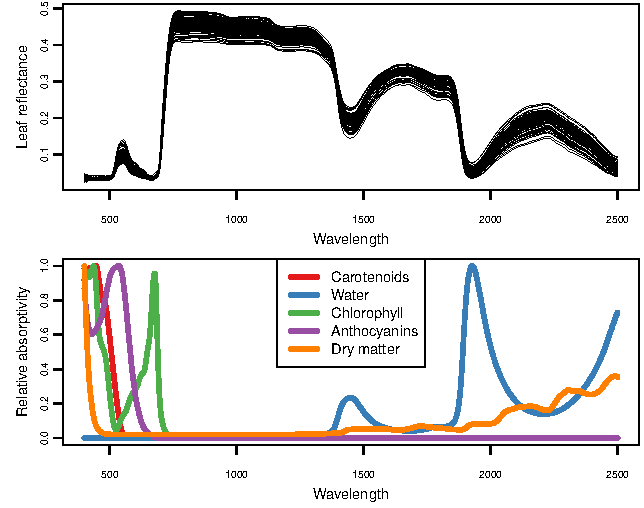
\includegraphics[width=\textwidth]{{figures/sigspec2-1}.pdf}
  \caption{\
    (Top) Example reflectance spectra of \textit{Acer rubrum} leaves.
    (Bottom) Normalized absorption coefficients for optical traits in this study.
  }\label{fig:prospect_coefficients}
\end{figure}

The six traits described above are used by the PROSPECT leaf radiative transfer model to simulate leaf reflectance and transmittance~\cite{jacquemoud_1990_prospect,feret_2008_prospect,feret_2017_prospectd}.
PROSPECT has been used extensively for the simulation of leaf and, (combined with canopy models) canopy reflectance~\cite{jacquemoud_2009_prosail}.
PROSPECT has also been used to estimate leaf spectral characteristics through spectral inversion (CITE).
Unlike empirical approaches for estimating leaf properties from spectra, including spectral indices~\cite{lemaire_2004_towards,feret_2011_optimizing} and partial least squares regression (PLSR)~\cite{serbin_2011_leaf}, PROSPECT aims to provide a causal understanding of leaf optical properties.
This means that, by design, PROSPECT intends to be generic across all species and conditions, and, more importantly, makes it a useful tool for applications where the links between leaf properties and spectra are important, such as modeling leaf absorbance for photosynthesis and for improving representations of energy balance in terrestrial biosphere models.
However, the extent of PROSPECT's generality has not been well tested, with most PROSPECT studies focusing on a relatively small set of species that are fairly similar to those used for PROSPECT's original calibration~\cite{feret_2008_prospect,feret_2011_optimizing,feret_2017_prospectd,li_2011_retrieval,wang_2015_leaf}.

The above discussion culminates in the following three questions:
First, how well can leaf optical traits be estimated from PROSPECT inversion over a wide range of species and experimental designs?
Second, how do leaf optical traits vary across a variety of environmental conditions and species?
Specifically, how is intraspecific variability in optical traits related to various growing conditions including local climate, canopy light environment, and exposure to pathogens?
As well, how well can interspecific variability in traits be explained by species attributes frequently used for grouping species into functional types? 
Third, how are leaf optical traits related to other leaf traits not directly estimable from PROSPECT inversion?
To address these questions, I applied my PROSPECT inversion methodology (Chapter 2) to a large database of leaf spectra and traits collected in a variety of natural and experimental settings.

\section{Methods}

\subsection{Data}

Data from this project were assembled from 22 projects on leaf spectra and related foliar traits (Table~\ref{tab:projectinfo}).
Most of these datasets are obtained directly from the ECOSIS spectral library (https://ecosis.org/).
Collectively, these data are comprised of nearly 12,000 observations from 346 species, and span a wide geographic (Figure~\ref{fig:datamap}) and climatic range (Figure~\ref{fig:dataclimate}).

%TODO: Maybe a summary of experimental treatments?
% Milkweed stress

\begin{table}
    \caption{Project information}
    \centering
    \begin{table}[H]
\centering\begingroup\fontsize{8}{10}\selectfont

\begin{tabular}{l>{\raggedright\arraybackslash}p{25em}rrr}
\toprule
Short name & Long name & Samples & Species & Sites\\
\midrule
ACCP & Accelerated Canopy Chemistry Program (ACCP) & 850 & 46 & 5\\
ANGERS & Angers, France spectra from INRA & 274 & 37 & 1\\
Barnes 2017 & Barnes et al. 2017. Beyond greenness: Detecting temporal changes in photosynthetic capacity with hyperspectral reflectance data. PLoS ONE. & 86 & 1 & 1\\
Cali. Eco. Traits & Fresh Leaf Spectra to Estimate Leaf Traits for California Ecosystems & 261 & 16 & 34\\
Cedar Creek Biodiv. & 2014 Cedar Creek ESR Grassland Biodiversity Experiment: Leaf-level Contact Data: Trait Predictions & 780 & 17 & 1\\
\addlinespace
Corn var. & Spectral Characterization of Multiple Corn Varieties: West Madison Agricultural Station 2014 & 288 & 1 & 1\\
Di Vittorio 2009 & Di Vittorio 2009 & 504 & 2 & 3\\
Hawaii 2000 & Hawaii 2000 vegetation species spectra & 588 & 56 & 48\\
LOPEX & Leaf Optical Properties Experiment (1993) & 66 & 45 & 1\\
Milkweed stress & Common Milkweed Leaf Responses to Water Stress and Elevated Temperature & 735 & 1 & 1\\
\addlinespace
Missoula TS & Missoula Montana lodgepole pine \& big sagebrush time series & 100 & 2 & 4\\
NASA FFT & NASA Forest Functional Types (FFT) & 1369 & 66 & 130\\
NASA HyspIRI & NASA HyspIRI field campaign & 1704 & 38 & 12\\
NGEE Arctic & Next Generation Ecosystem Experiment (NGEE) - Arctic & 614 & 13 & 3\\
NGEE Tropics & Next Generation Ecosystem Experiment (NGEE) - Tropics & 706 & 28 & 1\\
\addlinespace
Pepper K/N & Fresh and Dry Pepper Leaf Spectra with Associated Potassium and Nitrogen Measurements & 119 & 1 & 1\\
PVY solanum & Varietal Discrimination and Detection of PVY in Solanum tuberosum: Hawaii 2014 & 761 & 1 & 1\\
Santa Monica Mtns. & Santa Monica Mountains vegetation species spectra & 353 & 24 & 1\\
Soybean aphid & Productivity and Characterization of Soybean Foliar Traits Under Aphid Pressure & 1131 & 1 & 1\\
Spectral variation & Spectral Variation Between Leaf-level and Canopy-level Measurements & 16 & 1 & 1\\
\addlinespace
Wu 2016 & Wu et al. 2016 New Phytologist canopy traits study & 160 & 17 & 1\\
Yang 2016 & Yang et al. 2016 Remote Sensing of Environment & 497 & 3 & 2\\
\bottomrule
\end{tabular}\endgroup{}
\end{table}
\label{tab:projectinfo}
\end{table}

\begin{figure}
    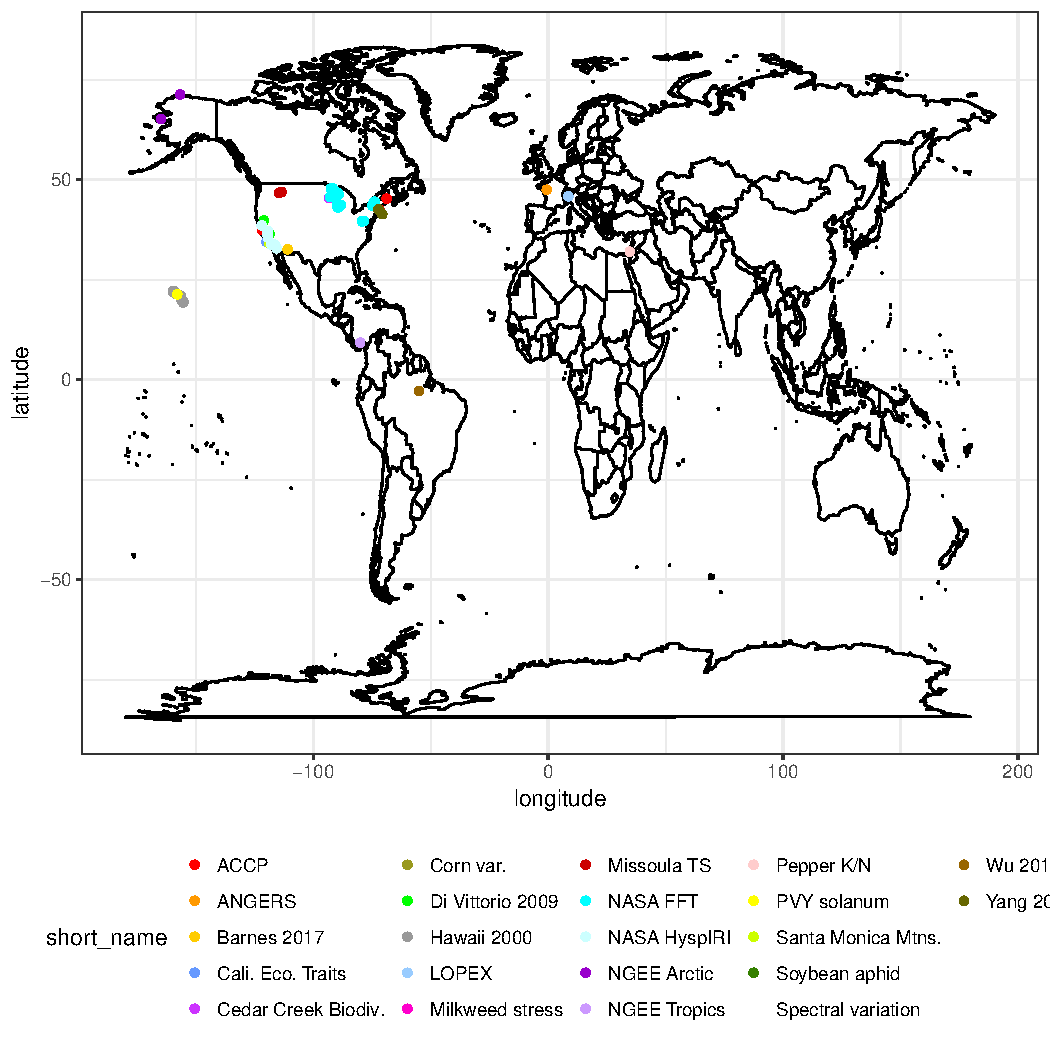
\includegraphics[width=\textwidth]{{figures/data_map}.pdf}
    \caption{Map of data locations}\label{fig:datamap}
\end{figure}

\begin{figure}
    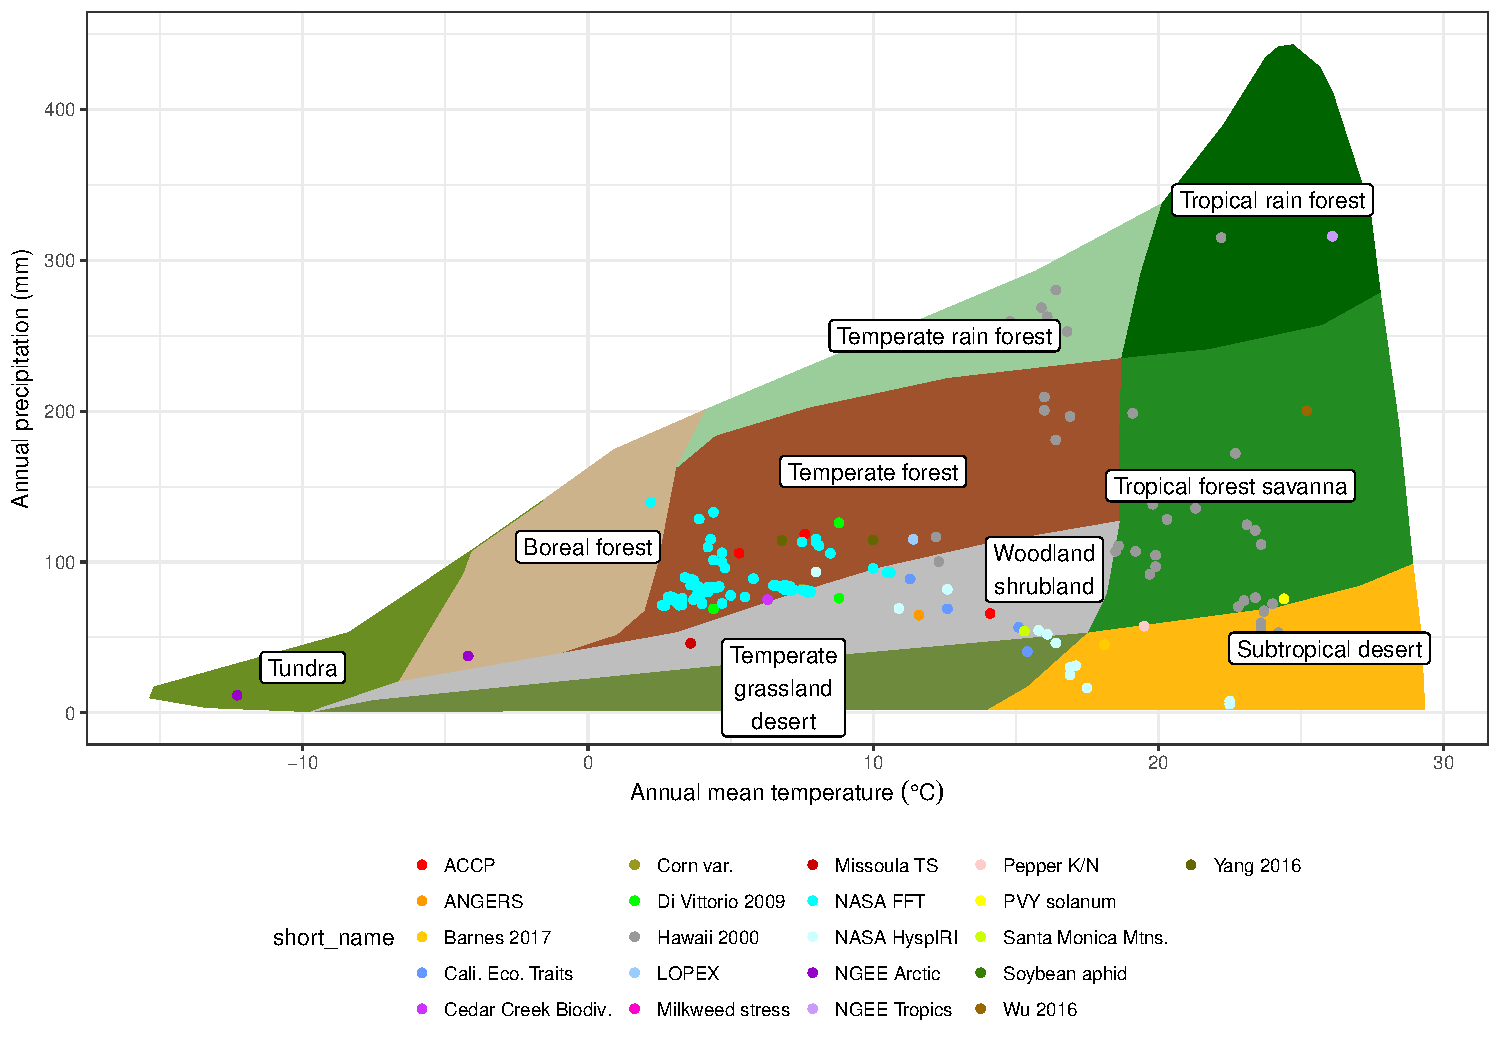
\includegraphics[width=\textwidth]{{figures/data_climate}.pdf}
    \caption{Data locations in climate space}\label{fig:dataclimate}
\end{figure}

\subsection{Trait estimation via PROSPECT inversion}

\begin{figure}
  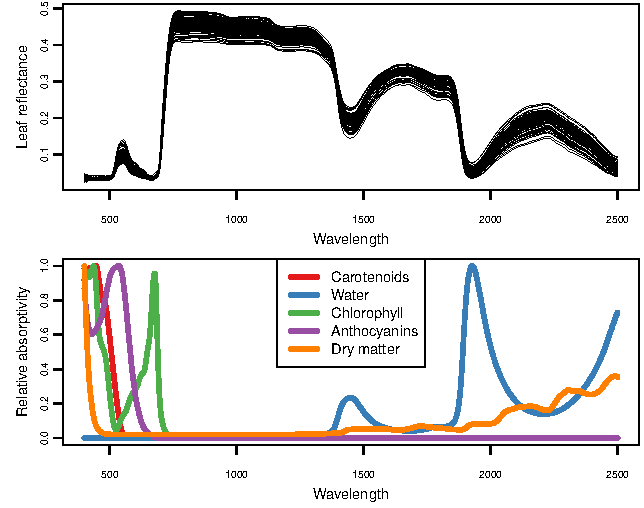
\includegraphics[width=\textwidth]{{figures/sigspec2-1}.pdf}
  \caption{\
    (Top) Example reflectance spectra of \textit{Acer rubrum} leaves.
    (Bottom) Normalized absorption coefficients for traits estimated by PROSPECT.
  }\label{fig:prospect_coefficients}
\end{figure}

The PROSPECT leaf radiative transfer model~\cite{jacquemoud1990_prospect,jacquemoud_2009_prosail,feret2008_prospect,feret2017_prospectd} simulates leaf reflectance and transmittance for 400 to 2500 nm wavelengths at 1 nm increments as a function of leaf morphological and biochemical characteristics.
In this chapter, I compared the performance of four different versions of PROSPECT, each of which uses a different combination of leaf traits:
PROSPECT 4 uses
total chlorophyll content per area ($\mu g~cm^{-2}$),
leaf water content per area ($g~m^{-2}$),
and leaf dry matter content per area ($g~m^{-2}$)~\cite{feret2008_prospect}.
PROSPECT 5 extends PROSPECT 4 with a parameter for
total carotenoid content per area ($\mu g~cm^{-2}$)~\cite{feret2008_prospect}.
PROSPECT 5B adds an additional parameter for
total ``senescent brown pigment'' content (arbitrary units)~\cite{jacquemoud_2009_prosail}.
Finally, PROSPECT D adds an additional parameter for
total anthocynanin content per area ($\mu g~cm^{-2}$)~\cite{feret2017_prospectd}.
The absorption coefficients for PROSPECT-D aligned with example leaf reflectance spectra are shown in Figure~\ref{fig:prospect_coefficients}.

To estimate traits from leaf spectra, I generally followed the Bayesian RTM inversion approach of~\cite{shiklomanov2016_rse}, except that I replaced the Metropolis-Hastings algorithm with a more efficient Differential Evolution algorithm with ``snooker'' update as implemented in the \texttt{BayesianTools} R package~\cite{bayesiantools}.
Forward simulations and Bayesian inversion of PROSPECT are implemented in the R package \texttt{PEcAnRTM}~\cite{shiklomanov2016_rse}, which is open source and freely available at https://github.com/pecanproject/pecan/modules/rtm.
Where leaf spectra extended beyond the 400 to 2500 nm wavelength range of the PROSPECT model, I used only the observations from 400 to 2500 nm.
Where leaf spectra were sampled at a spectral resolution coarser than 1 nm or did not include all wavelengths simulated by PROSPECT, I subset the PROSPECT output in the likelihood function to match the observations.
Where leaf spectra were sampled at a finer spectral resolution than 1 nm, or where wavelengths did not align at 1 nm intervals, I used cubic spline interpolation (default method in the base R function \texttt{spline}) to align the spectra with PROSPECT output.
Where leaf spectra were provided as ``pseudo-absorbance'' ($1 - \log_{10}(R)$), I added the corresponding transformation to the PROSPECT output in the likelihood calculation. 

\subsection{Analysis}

To compare PROSPECT versions, I plotted traits estimated by more than one version of PROSPECT as pairwise scatter plots, fit a least-squares linear regression to each and compared the result to a 1-to-1 line, and calculated the pairwise correlation coefficient (Figures~\ref{fig:prospect_pairs_N}-\ref{fig:prospect_pairs_Cm}).
To validate PROSPECT inversions, I compared trait estimates from PROSPECT inversion with direct measurements of the corresponding traits, where these traits were available.
To explore project-specific biases in the inversion, I fit least-squares linear regressions to investigate the ability of trait estimates from spectra to predict the measured traits, and I report the slopes, intercepts, and $R^2$ values of those regressions (Figure~\ref{fig:project_validation_summary}, Supplementary Tables~\ref{tab:r2_byproject_Cab}-\ref{tab:r2_byproject_Cm}).
To identify species-specific errors, I also performed this analysis for each project-species combination with at least 5 observations (Figures~\ref{fig:error_speciesbyproj_Cab}-\ref{fig:error_speciesbyproj_Cm}).

To investigate the effects of experimental treatments and environmental conditions, I fit a linear fixed effects model for each optical trait and each treatment, with an additional fixed effect for species if multiple species were present in that treatment.
To investigate the role of intraspecific variability in climate, I subset the data to species that were present at at least 10 different sites and fit a fixed-effects model to each optical trait as a function of species, annual mean temperature, and annual precipitation.
I then present the direction of each GLM coefficient and whether the coefficient was significant (Figure~\ref{fig:treatment_summary}).

One study in this dataset---Yang et al.~(2016) \nocite{yang_2016_seasonal}---explicitly looked at the seasonal trajectories of leaf reflectance, allowing me the chance to look at the phenology of leaf optical traits (Figure~\ref{fig:trait_phenology}).

To investigate the correlations between optical traits and other traits measured directly, I calculated the pairwise non-missing correlations (R function \texttt{cor} with option \texttt{use = pairwise.complete.obs}) and plotted the resulting correlation coefficients using the \texttt{corrplot} package.
I performed this analysis for both individual observations and species means, where a trait was observed for at least 3 species.

I performed all analyses using R version 3.4.4~\cite{rstats}.
The data and code for performing these analyses are open source and freely available at https://github.com/ashiklom/rspecan.

\section{Results}

\subsection{Estimating traits via PROSPECT inversion}

\begin{figure}
  \centering
  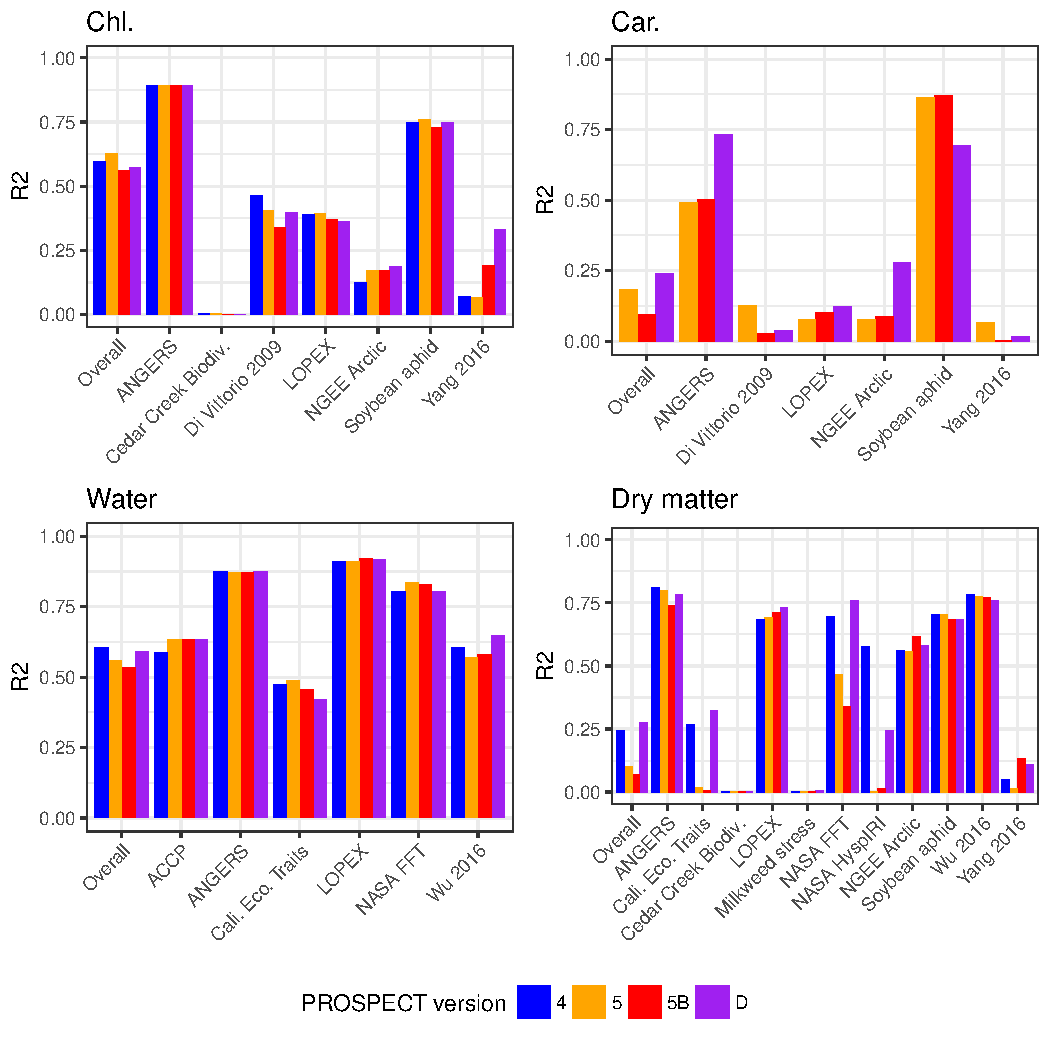
\includegraphics[width=\textwidth]{{figures/project_validation_summary}.pdf}
  \caption{\
    Validation of PROSPECT against observed trait values, by project and PROSPECT version.
    Y-axis represents $R^2$ values for robust linear regression.
  }\label{fig:project_validation_summary}
\end{figure}

Across most projects and traits, the four different PROSPECT versions performed similarly in terms of their ability to retrieve traits (Figure~\ref{fig:project_validation_summary}).
For all versions of PROSPECT, leaf water content was consistently the most accurate trait retrieved, while retrievals of other traits were highly project-specific.
For several projects spanning a large range of species (Cali.\ Eco.\ Traits, NASA FFT, and NASA HyspIRI), moving from chlorophyll as the only pigment (PROSPECT 4) to chlorophyll and carotenoids (PROSPECT 5/5B) drastically reduced inversion accuracy of dry matter contents, but this accuracy was restored by the further addition of anthocyanins and modification of the refractive index in PROSPECT D (Figure~\ref{fig:project_validation_summary}).
Because PROSPECT-D also retrieves anthocyanin content and generally performed as well or better than other versions, it was the version selected for subsequent analyses.

\begin{figure}
  \centering
  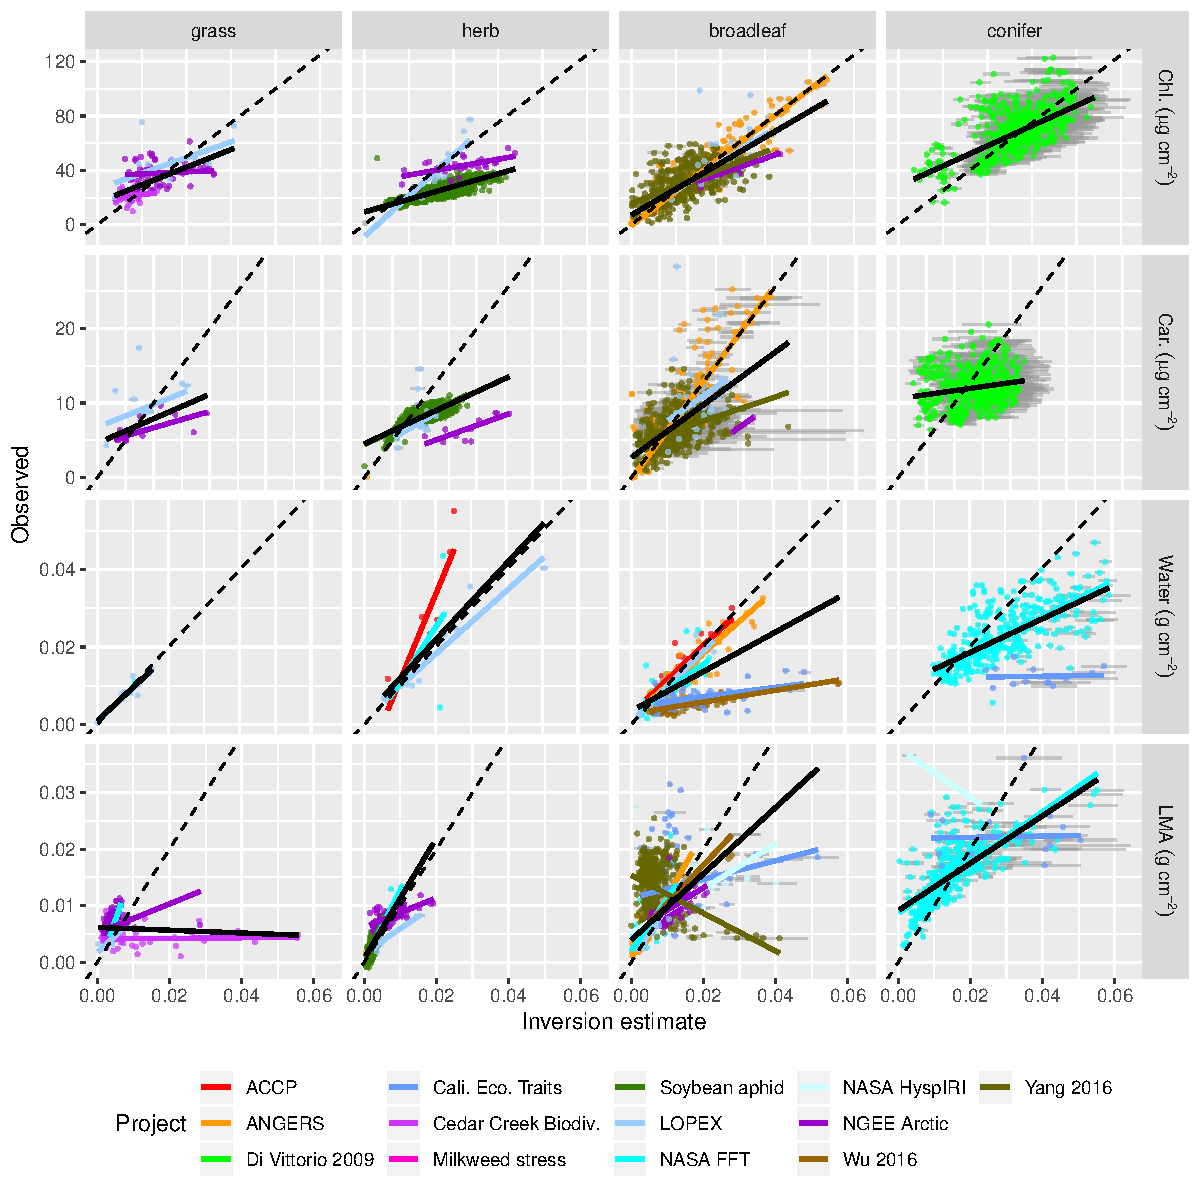
\includegraphics[width=\textwidth]{3_prospect/figures/validation_by_gf.pdf}
  \caption{\
    Validation of PROSPECT-D against observed trait values.
    Grey lines indicate 95\% confidence intervals around trait estimates.
    Solid, colored lines are robust regressions fit to the data by project and functional type.
    The solid black line is a regression fit to all of the data for a given functional type.
    The dashed black line is a 1 to 1 fit.
  }\label{fig:prospect_D_validation}
\end{figure}

\begin{figure}
  \centering
  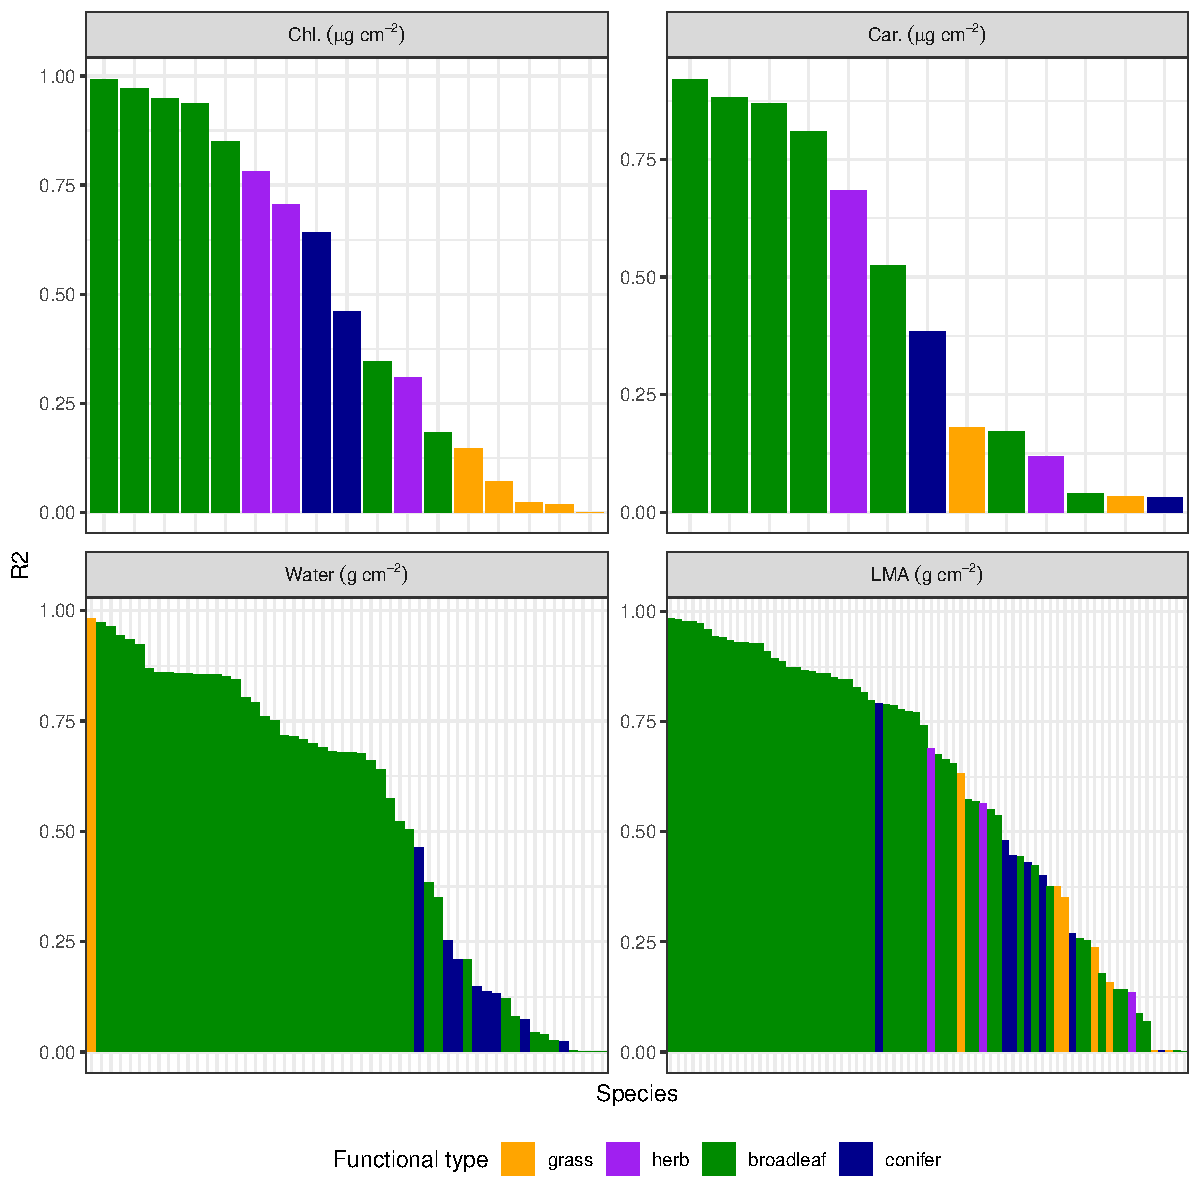
\includegraphics[width=\textwidth]{3_prospect/figures/r2_by_gf.pdf}
  \caption{%
    $R^2$ values from robust linear regression of direct trait observations as a function of PROSPECT-D inversion estimates.
    Colors indicate functional type, as determined by the interaction of growth form and leaf morphology.
  }\label{fig:prospect_D_r2}
\end{figure}

Inversion accuracy varied significantly by project and growth form (Figures~\ref{fig:project_validation_summary},~\ref{fig:prospect_D_validation}, and~\ref{fig:prospect_D_r2}).
In terms of regression $R^2$, inversion accuracy was highest for broadleaved trees, lower for herbs and needleleaved trees, and lowest for grasses.
However, there was substantial project-specific variability in accuracy between these groups.
For example, both water and LMA retrievals from the California Ecosystem Traits dataset were consistently much worse than for other datasets for both broadleaved and needleleaved trees, while the LOPEX and ANGERS datasets (against which PROSPECT is calibrated) performed very well for all traits for broadleaved trees, herbs, and grasses.
The full pairs plot (Figure~\ref{fig:prospect_D_validation}) reveals that regression $R^2$ is insufficient for capturing all of the patterns in the validation.
In several cases (e.g.\ water and LMA retrieval for conifers from the NASA FFT dataset, or carotenoid retrievals from the soybean aphid dataset), there is a saturation effect, whereby accuracy is good at lower trait values but declines as trait values increase.
In other cases, there is a significant additive and/or multiplicative bias in retrievals --- for instance, in the retrieval of chlorophyll and carotenoid contents from herbs.

\subsection{Drivers of variability in leaf optical traits}

\begin{figure}
  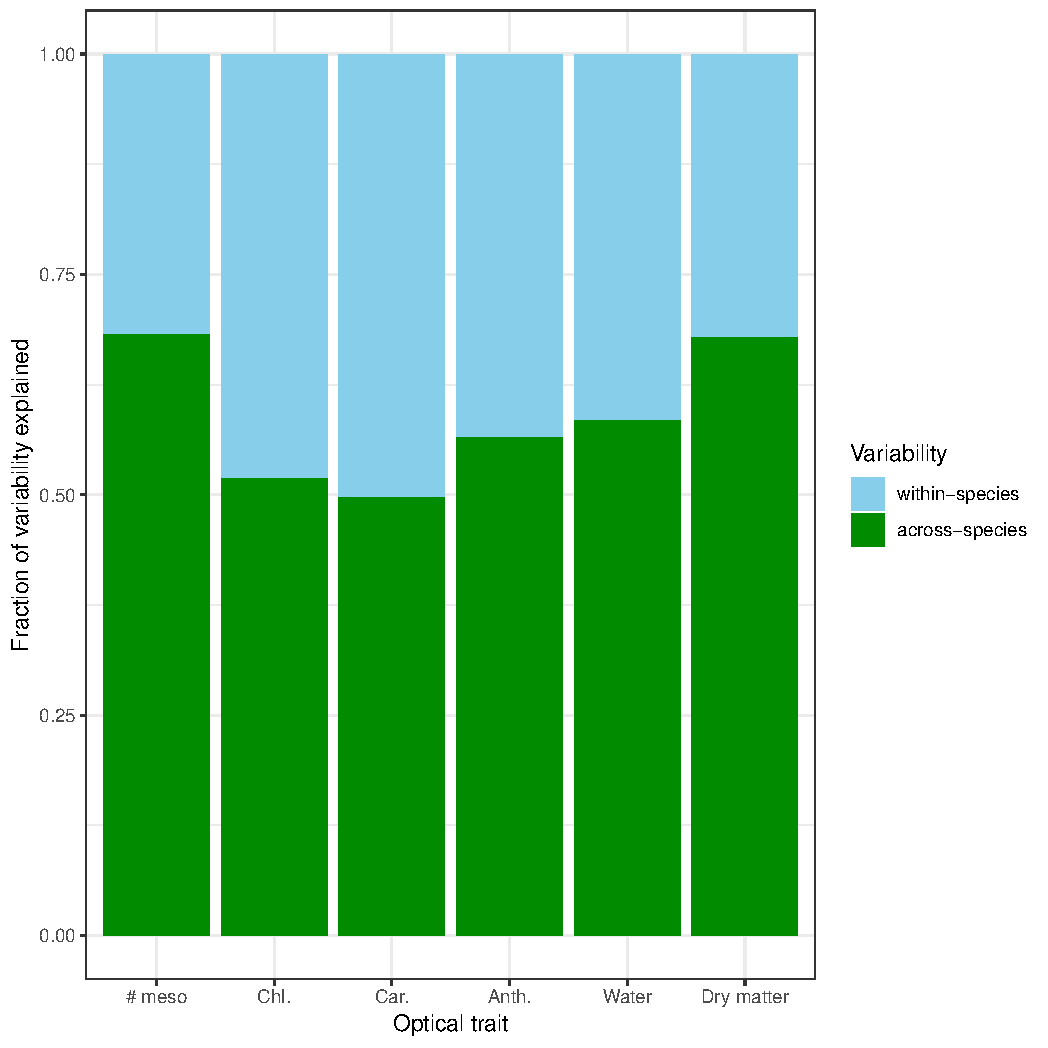
\includegraphics[width=\textwidth]{{figures/within_vs_across}.pdf}
  \caption{\
    Fraction of variance in each optical trait explained by species identity,
    based on analysis of variance on least-squares linear regression.
  }\label{fig:within_vs_across}
\end{figure}

\begin{figure}
  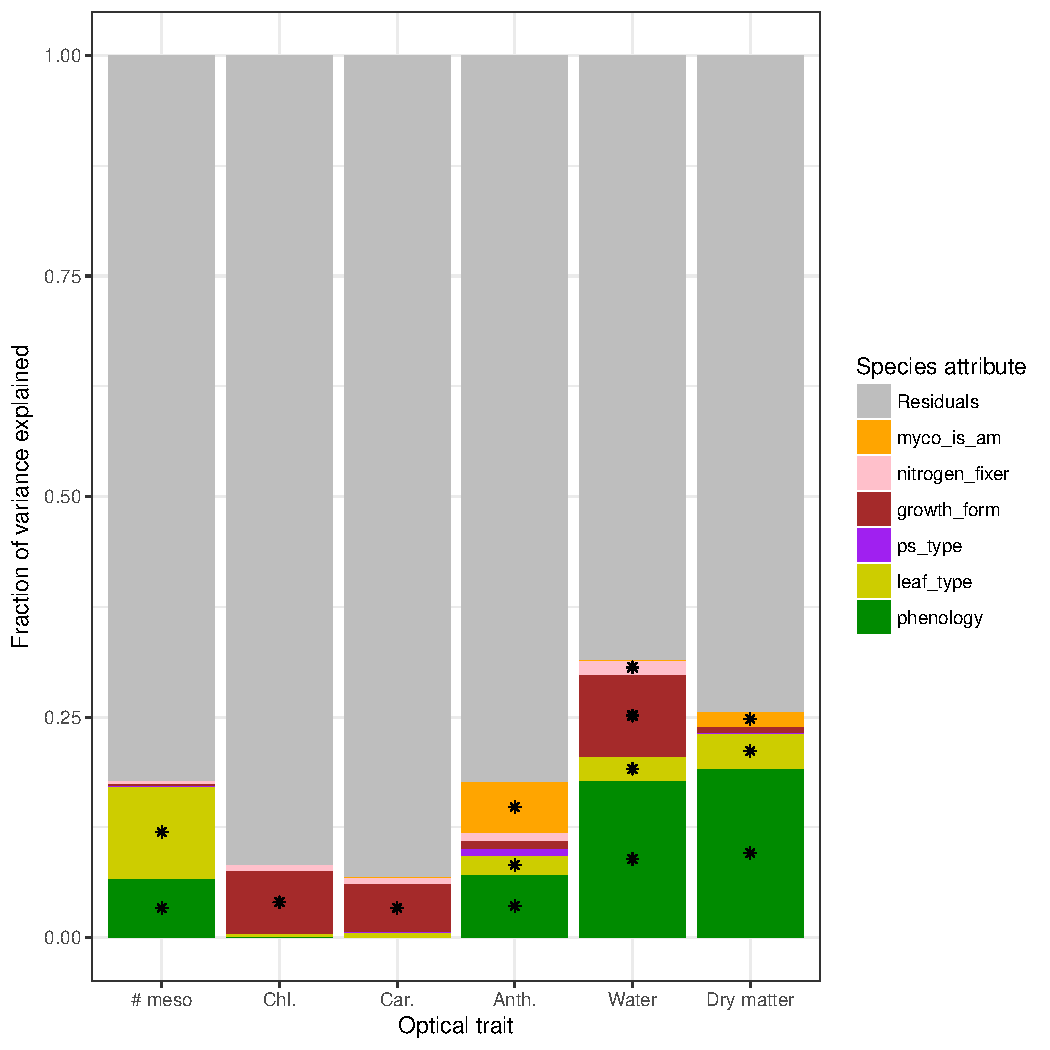
\includegraphics[width=\textwidth]{{figures/across_species_anova}.pdf}
  \caption{\
    Fraction of across-species variance in each optical trait (i.e.~species means) explained by species attributes,
    based on analysis of variance on least-squares linear regression.
    A star (*) indicates attribute effects significant at the 90\% confidence interval.
    Attributes are as follows:
    \texttt{myco\_is\_am} --- Mycorrhizal fungi association (arbuscular or other such as ectomycorrhizal or ericoid);
    \texttt{nitrogen\_fixer} --- whether the species is a Nitrogen fixer;
    \texttt{growth\_form} --- tree, shrub, herb, or grass;
    \texttt{ps\_type} --- photosynthetic pathway (C3 or C4);
    \texttt{leaf\_type} --- leaf morphology (broadleaved or needleleaved);
    \texttt{phenology} --- whether the species is deciduous or evergreen.
  }\label{fig:across_species_anova}
\end{figure}

Across all optical traits, roughly half of variability was explained by species identity (Figure~\ref{fig:within_vs_across}).
The variance across species means was largely idiosyncratic to species, with only up to 25\% of variance explainable by species attributes (Figure~\ref{fig:across_species_anova}).
The most important explanatory attribute was leaf phenology (deciduous vs.~evergreen), with occasional significant effects for leaf type (broad vs.~needle), growth form (woody vs.~herbaceous), and mycorrhizal association (arbuscular or non-arbuscular). 

\begin{figure}
  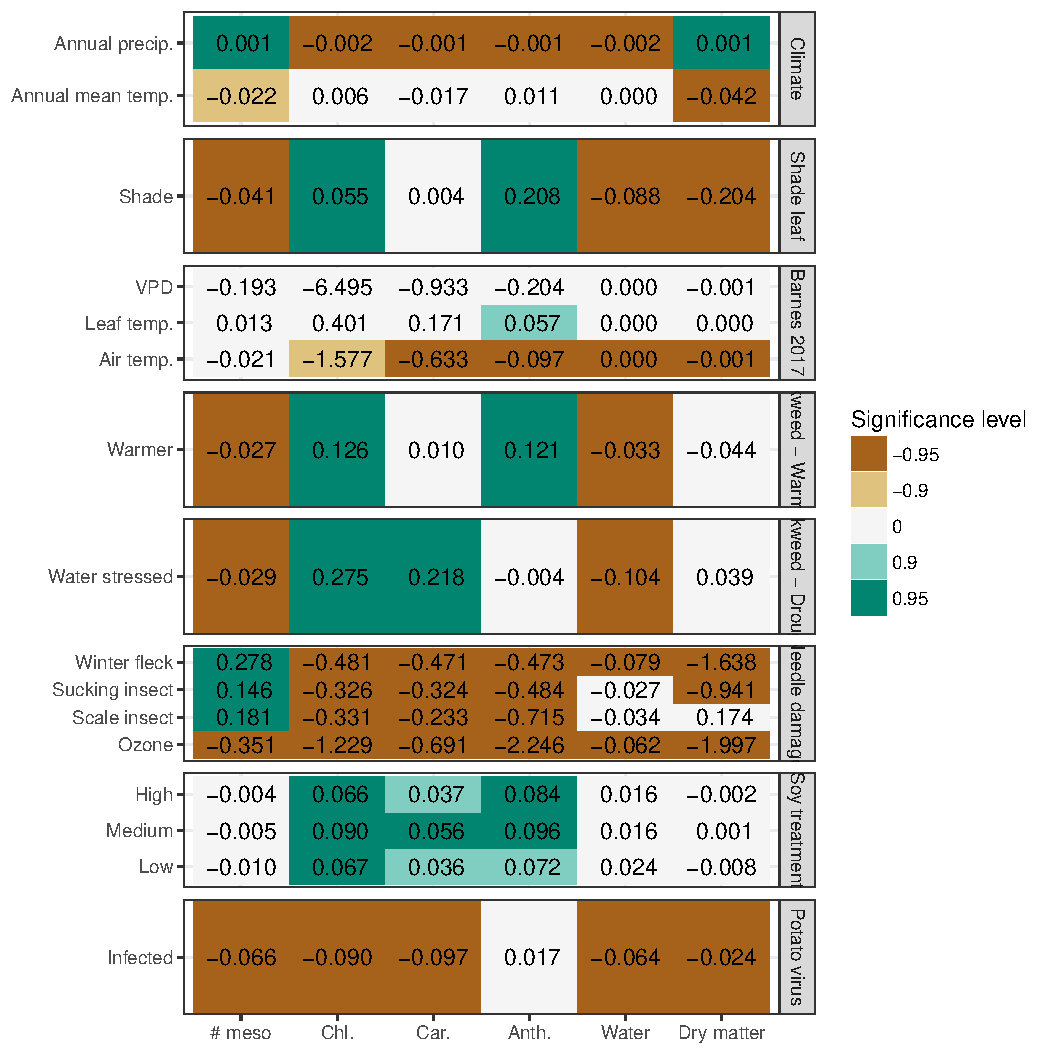
\includegraphics[width=\textwidth]{{figures/treatment_summary}.pdf}
  \caption{\
    Effects of different sources of intraspecific variability on traits estimated via PROSPECT inversion.
    Each value is the fixed effect slope on the corresponding trait normalized to zero mean and unit variance, as estimated from a linear fixed-effects model.
    Color brightness indicates degree of statistical significance (90 or 95\% confidence level), and color hues indicate effect direction (positive or negative).
  }\label{fig:treatment_summary}
\end{figure}

Leaf optical traits responded significantly to a range of natural and experimental stressors (Figure~\ref{fig:treatment_summary}).
Across the entire dataset, intraspecific variability in optical traits was weakly but, in some cases, significantly related to climate, with the strongest effects being declines in mesophyll structure and dry matter content with increasing temperature.
Canopy light environment (i.e.\ whether a leaf was sunlit or shaded) also had a significant effect on most traits, at least for species on which a comparison was possible.
Specifically, shaded leaves showed higher chlorophyll and anthocyanin concentrations and reduced mesophyll structure and water and dry matter contents.

Based on leaf reflectance measurements of \textit{Populus deltoides} (eastern cottonwood) at the University of Arizona by Barnes et al.~(2017), \nocite{barnes_2017_beyond}
seasonal variations in vapor pressure deficit---but not leaf temperature---had significant negative effects on all traits, with the strongest effects on chlorophyll and anthocyanin contents.
Similarly, warming and drought experiments on \textit{Asclepias syriaca} (common milkweed)  had strong and significant effects on almost all optical traits, with both treatments leading to significant decreases in leaf water content and effective number of mesophyll layers and increases in pigments and dry matter content concentrations~\cite{milkweed_data}.
Leaf optical traits also responded significantly to chemical and biotic stressors.
Based on data from Di Vittorio (2009) \nocite{divittorio_2009_enhancing}, needles of \textit{Pinus ponderosa} and \textit{Pinus jeffreyi} from the northern Sierra Nevada mountains experienced reductions in all traits, but most strongly in pigment and dry matter contents,
when afflicted with winter fleck (patchy mortality of needle epidermal cells, usually triggered by exposure to harsh winter weather), sucking and scale insect, and especially ozone damage.
As well, spectral inversion revealed small but statistically significant declines across all optical traits except anthocyanins in \textit{Solanum tuberosum} (potato) plants infected with potato virus Y~\cite{solanum_pvy_data}.
On the other hand, treatment of \textit{Glycine max} (soybean) with aphids resulted in a small but significant increase in pigment concentrations, with the strongest effect observed at medium-level treatment~\cite{soybean_data}.

\begin{figure}
  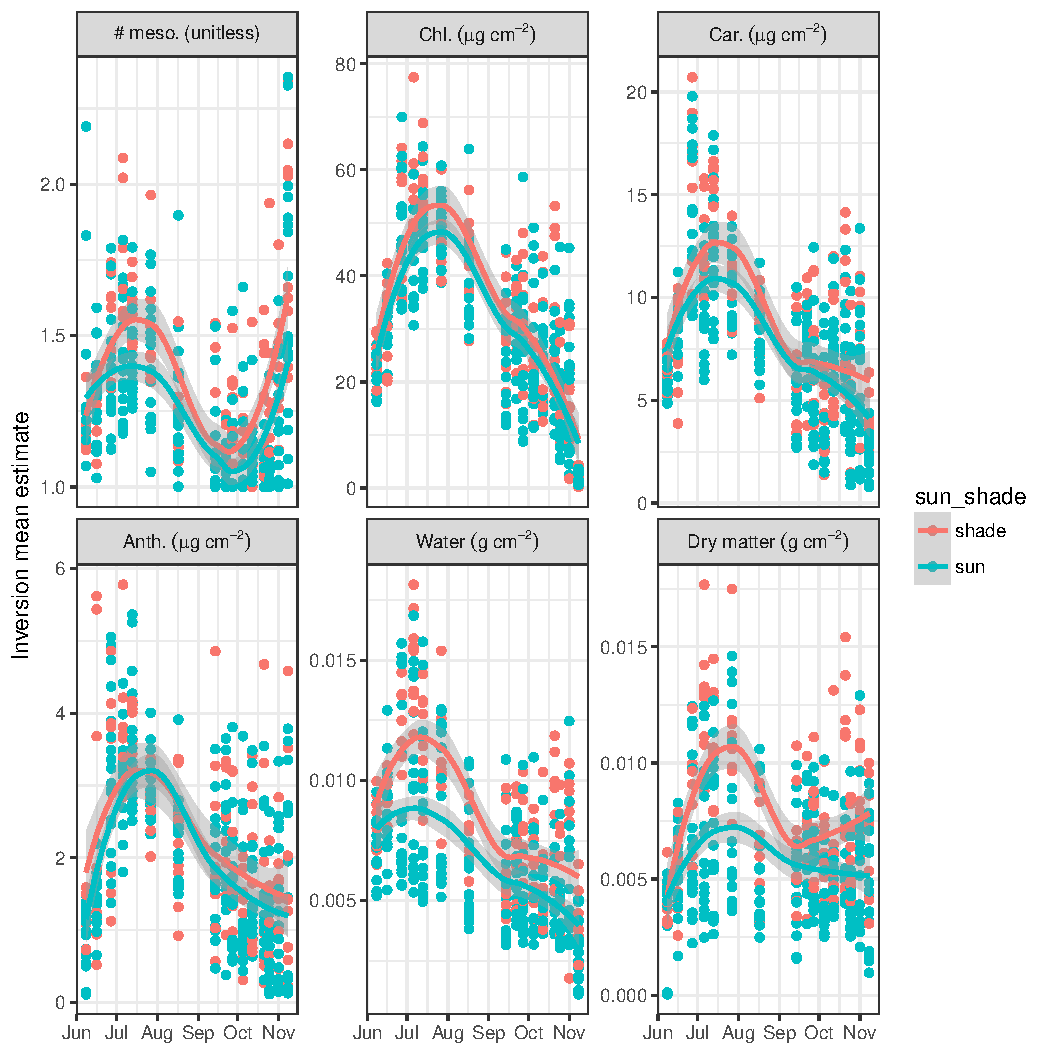
\includegraphics[width=\textwidth]{{figures/trait_phenology}.pdf}
  \caption{\
    Optical trait estimates through a season for \textit{Quercus rubra} (red oak) at Martha's Vineyard, MA by Yang et al.~(2016).
    Colors indicate sunlit vs.~shaded leaves.
    Line is a LOESS best fit with shaded standard error.
  }\label{fig:trait_phenology}
  \nocite{yang_2016_seasonal}
\end{figure}

Where such measurements were available, leaf optical traits exhibited a strong phenological signal (Figure~\ref{fig:trait_phenology}).
All optical traits showed a peak in late July / early August, followed by a decline into the fall, with the sharpest declines for pigments and water content and less precipitous declines for dry matter and mesophyll structure.
Furthermore, the effective number of leaf mesophyll layers, and to a lesser extent, leaf dry matter content in shade leaves, appeared to increase in the late fall.
With the exception of anthocyanin content, all traits for shaded leaves were higher and experienced a greater seasonal variability than sunlit leaves.

\subsection{Trait correlations}

\begin{figure}
  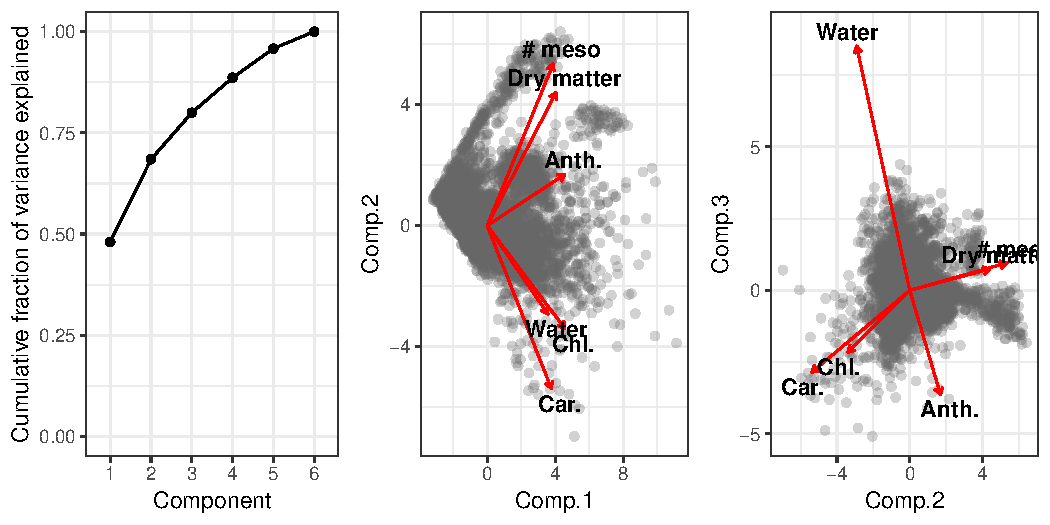
\includegraphics[width=\textwidth]{figures/prospect_pca.pdf}
  \caption{\
    Principal components analysis of optical trait correlation matrix. 
    (Left) Cumulative fraction of variance explained by each principal component.
    (Center, Right) Principal component scores and vectors for each optical trait for components 1 and 2 (center) and 2 and 3 (right).
  }\label{fig:prospect_pca}
\end{figure}

Optical traits estimated by PROSPECT are not mutually independent, but rather have some structure to their covariance (Figure~\ref{fig:prospect_pca}).
The first principal component, which explains roughly 50\% of the variability, is defined by increases in all leaf traits and can be interpreted as overall leaf size and tissue density.
The second principal component, which explains an additional 20\% of the variability, is characterized by an approximate trade-off between structural (mesophyll structure and dry matter content) and physiological (chlorophyll, carotenoid, and water contents).
The third principal component, which explains a further 15\% of the variability, is dominated by a trade-off in water and anthocyanin concentrations.

\begin{figure}
  \centering
  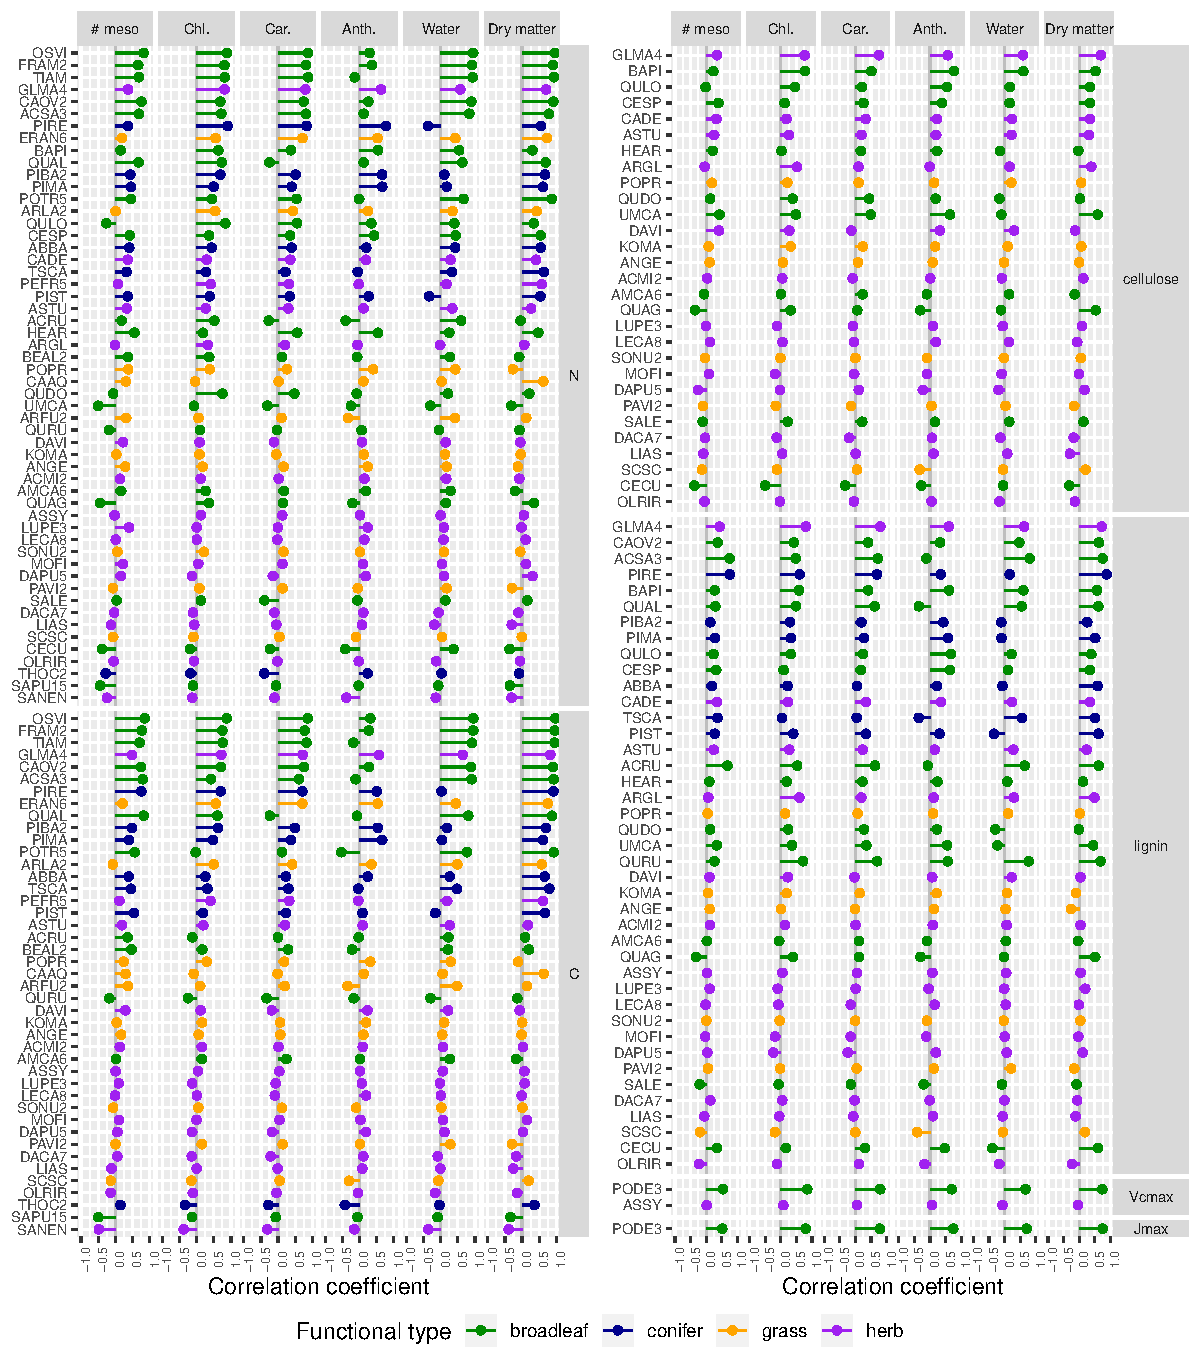
\includegraphics[width=\textwidth]{3_prospect/figures/trait_correlations_lollipop.pdf}
  \caption{\
    Intra-specific pairwise correlations of optical traits with direct measurements of area-based
    leaf N, C, cellulose, lignin, $V_{c,\max}$, and $J_{\max}$.
    Colors indicate plant functional type.
    Species are displayed along the y axis, and are sorted within each facet from highest to lowest average correlation across all traits.
    Analysis was performed only for species with at least 10 pairwise observations of each trait.
  }\label{fig:trait_correlations}
\end{figure}

Covariance of optical traits with six area-normalized traits---leaf nitrogen, carbon, cellulose, and lignin contents, $V_{c,\max}$, and $J_{\max}$---was strongly species specific, but, in many cases, substantial (Figure~\ref{fig:trait_correlations}).
In general, for any given species, most of the estimated optical traits exhibited similar correlations with the directly measured trait.
For instance, for Glycine (\textit{Glycine max}, GLMA4), all optical traits were positively correlated with leaf N, C, cellulose, and lignin, whereas for milkweed (\textit{Asclepias syriaca}, ASSY), all of these correlations were negligible.
Leaf nitrogen correlated best for the largest number of species with leaf chlorophyll and, to a slightly lesser extent, with dry matter content.
Leaf carbon and lignin were most consistently correlated with leaf dry matter content, while correlations with cellulose were more idiosyncratic.
$V_{c,\max}$ and $J_{\max}$ were strongly positively correlated with all traits for \textit{Populus deltoides} (PODE3), but completely uncorrelated for milkweed (ASSY).
Correlations between optical and other traits were generally strongest for broadleaf trees, somewhat weaker for needleleaved trees, and weakest for herbs and grasses.
Although this was also the general pattern in the validation, exploratory analyses (not shown) do not find any consistent relationship between validation $R^2$ and correlation.

\begin{figure}
  \centering
  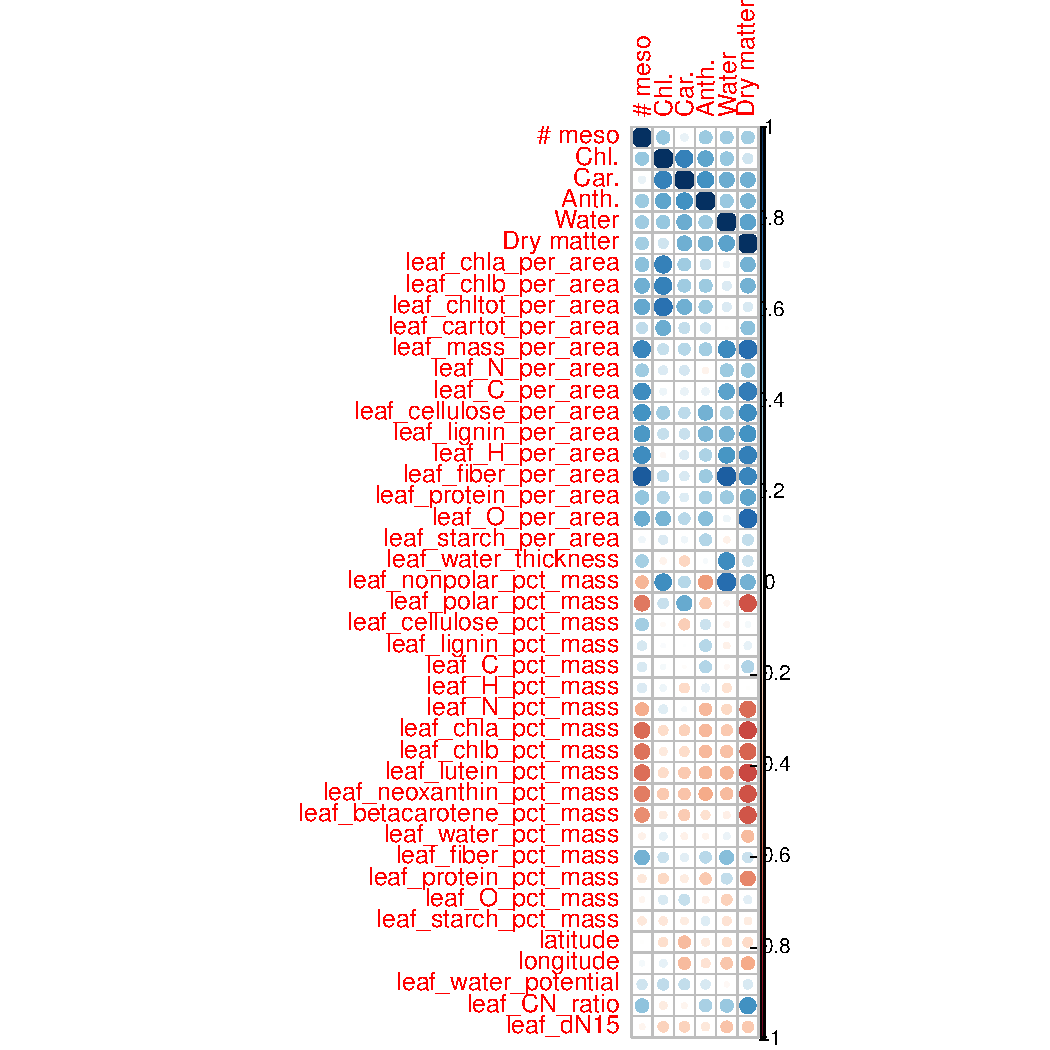
\includegraphics[width=\textwidth]{3_prospect/figures/trait_correlations_species.pdf}
  \caption{%
    Pairwise correlations among species means for PROSPECT inversion estimates and other, directly-measured area-normalized traits.
    In lower diagonal, circle color and size indicate correlation direction and strength, respectively.
    Values in upper diagonal are correlation coefficients, colored by direction and strength.
  }\label{fig:trait_correlations_species}
\end{figure}

Among species means, almost all area-based traits were at least weakly positively correlated with each other (Figure~\ref{fig:trait_correlations_species}).
Among optical traits, the strongest correlations were among the three pigments, and of leaf water and dry matter contents.
Spectrally-estimated leaf mesophyll structure and dry matter content correlated strongly with traits related to structure, namely C, cellulose, lignin, and fiber contents.
Leaf N was most strongly correlated with dry matter and water contents and leaf mesophyll structure, and only weakly correlated with chlorophyll and carotenoid contents.

\section{Discussion}

\subsection{Estimating traits through PROSPECT inversion}

Establishing general, species- and site-independent relationships between leaf functional traits and optical properties is challenging.
My results suggest that Bayesian PROSPECT inversion is a promising technique for achieving this objective.
Averaged across the entire dataset, spectral estimates of traits were able to capture 50 to 75\% of the variability in the true values of the traits (Figure~\ref{fig:project_validation_summary}).
In addition, spectral trait estimates were able to not only identify but also ascribe a physiological mechanism to intra-specific variability associated with long-term acclimation and acute stress responses in both natural and experimental settings (Figure~\ref{fig:treatment_summary}).
By comparing retrieval accuracy across different versions, my results also reaffirm the value of recent improvements to PROSPECT\@.
In particular, the successive additions of carotenoid~\cite{feret_2008_prospect} and anthocyanin~\cite{feret_2017_prospectd} pigments significantly increased accuracy of chlorophyll retrievals in the phenological dataset of Yang et al.~(2016) (Figures~\ref{fig:prospect_D_validation},~\ref{fig:project_validation_summary}, and~\ref{fig:validation_cab}), which points to the importance of modeling non-photosynthetic pigments in leaves sampled early or late in the growing season.

That being said, the large scale validation demonstrated here reveals enduring challenges and development opportunities for modeling leaf optical properties and retrieving leaf traits from spectra.
The particularly poor inversion accuracy for grasses (Figures~\ref{fig:prospect_D_validation} and~\ref{fig:prospect_D_r2}) suggests that the biochemistry and morphology of grasses do not fit the assumptions of PROSPECT\@.
Perhaps lower-hanging fruit is investigation of places where inversion estimates did well at capturing variability in traits, but were additively or multiplicatively biased.
For example, estimates of chlorophyll and carotenoid content in herbs from two dramatically different environments and species (greenhouse-grown soybean and tundra vegetation) showed virtually the same multiplicative bias and accuracy (Figure~\ref{fig:prospect_D_validation}).
One possible culprit for this bias is the chlorophyll $a$--$b$ ratio, which varies within and across species~\cite{kurahotta_1987_relationship,kitajima_2003_increases} but is fixed in the current version of PROSPECT\@.
Fortunately, a recently released update to PROSPECT succeeded in modeling chlorophyll $a$ and $b$ independently~\cite{zhang_2017_extended}.
This advance continues an ongoing positive trend in improving the detail with which PROSPECT models leaf optical properties.
 
One conclusion of Chapter 2 was that the use of physically-based absorption coefficients, such as that for leaf water content, is important for accurate trait retrievals using physically-based radiative transfer models.
Results from the wider range of species and projects in this chapter challenge this notion.
Retrievals of leaf water content and total chlorophyll concentration had comparable overall $R^2$ values (Figure~\ref{fig:project_validation_summary}).
However, leaf water content retrievals exhibited clear and significant project-specific biases, especially at high values (Figure~\ref{fig:prospect_D_validation})
Meanwhile, chlorophyll content retrieval was more consistently accurate across its entire range, even for needleleaved species (in the Di Vittorio dataset) (Figure~\ref{fig:prospect_D_validation}) that poorly fit the parallel-plane assumptions of the PROSPECT model~\cite{allen_1969_interaction,jacquemoud_1990_prospect} and, more importantly, despite the fact that the chlorophyll absorption coefficients for PROSPECT are calibrated only against the ANGERS dataset, which does not have any conifers~\cite{feret_2008_prospect,feret_2017_prospectd}.
Project-specific calibration has been shown to further improve the results of PROSPECT inversion~\cite{li_2013_retrieval}, which suggests that re-calibration of PROSPECT absorption coefficients against a wider range of species and environmental conditions (such as those used here) could lead to significant improvements in PROSPECT performance.
Ongoing efforts to curate and make publicly available spectral observations, such as the ECOSIS project (ecosis.org), significantly aid such efforts.

\subsection{Variation in optical traits}

Optical traits showed substantial variability both within and across species.
The extent of intra-specific variability in optical traits was substantial---from 30\% for leaf structure and dry matter content to nearly 50\% for pigment concentrations (Figure~\ref{fig:within_vs_across})---and fell comfortably in the range of intraspecific trait variability reported in other studies for similar traits~\cite{messier_how_2010,albert_multi-trait_2010}.
Following the definition of McGill et al.~(2006) that a useful ``trait'' is one that varies more across than within species, all six of the traits examined in this study technically qualify as ``traits'', but pigment concentrations only barely. \nocite{mcgill_2006_rebuilding}
In addition, the intraspecific variability is poorly explained by species attributes typically used to define plant functional types (e.g.\ for dynamic vegetation models)---taken together, species-specific attributes were able to explain at most around 30\% of interspecific variability (Figure~\ref{fig:across_species_anova}).
This result adds to the emerging body of literature on the limited ability of discrete plant functional types with fixed traits to effectively capture variability in plant and ecosystem function~\cite{vanbodegom2012_beyond,vanbodegom2014_fully,verheijen2015_variation,Clark_2016_Why}.

Some of the intraspecific variability in optical traits was not random, but rather suggested a systematic plastic response to biotic and abiotic stressors (Figures~\ref{fig:treatment_summary} and~\ref{fig:trait_phenology}).
For example, the observed increase in leaf dry matter content with decreasing temperature and increasing precipitation both agree with the meta-analysis of leaf mass per area by Poorter et al.~(2009). \nocite{poorter_2009_causes}
On the other hand, the absence of significant trends in pigment and water contents with respect to site temperature are likely because these traits respond more rapidly to environmental conditions, which is supported by their relatively higher fraction of intra-specific variability (Figure~\ref{fig:within_vs_across}).
This idea is further supported by the fact that pigment concentrations, but not leaf structure or dry matter content, responded significantly to within-season temperature fluctuations in the Barnes et al.~(2017) \nocite{barnes_2017_beyond} dataset and to aphid pressure in the soybean aphid dataset (Figure~\ref{fig:treatment_summary}).
This positive response of chlorophyll concentration to aphid pressure is surprising.
Alves et al.~(2015) \nocite{alves_2015_soybean} found significant effects of aphid infestation on soybean near-infrared reflectance and NDVI but no effect of on chlorophyll content.
Meanwhile, Luo et al.~(2012) \nocite{luo_2012_evaluation} found that wheat aphid infestation increased wheat leaf reflectance across the visible and near-infrared range, consistent with reduced pigment concentrations.
This result is unlikely to be caused by inaccurate PROSPECT estimates of pigment concentrations because inversion accuracy of both chlorophyll and carotenoids for this dataset was among the highest in this study (Figures~\ref{fig:project_validation_summary} and~\ref{fig:prospect_D_validation}).

I observed statistically significant differences in leaf morphology and biochemistry between sunlit and shaded leaves.
Chlorophyll content was significantly higher in shade leaves compared to sun leaves, which supports established theory that allocation of resources to light absorption relative to other photosynthetic functions (e.g.\ carbon fixation and electron transport) increases with decreasing irradiance~\cite{hikosaka_1995_model}.
At the same time, the reduced leaf dry matter content and mesophyll structure in shade leaves agrees with established understanding of the relationship between leaf mass per area and irradiance~\cite{poorter_2009_causes}.
However, the lack of a significant shade effect on carotenoid content and the positive effect on anthocyanins are surprising, given the current understanding of the photoprotective role of these pigments~\cite{young_1991_photoprotective,steyn_2002_anthocyanins}.
One explanation for the lack of a shade effect on carotenoids is that the response is non-linear, as has been shown in treatments with more finely varied light levels~\cite{sonobe_2017_estimating}.
An alternative, simpler explanation may be inaccuracy in retrievals related to the relative coarseness with which pigments are currently treated by PROSPECT (as discussed above).

Another source of intraspecific variability in optical traits explored in this study was phenology (Figure~\ref{fig:trait_phenology}).
PROSPECT inversion was able to successfully capture the phenological progression of chlorophyll and carotenoid contents as they increase early in the growing season and decline in the fall~\cite{yang_2014_beyond,yang_2016_seasonal}.
However, the results for leaf mass per area disagreed with the direct measurements in several important ways.
First, contrary to direct observations at this site~\cite{yang_2016_seasonal} and to expectations based on literature survey~\cite{poorter_2009_causes}, my estimates for leaf mass per area were consistently lower in sunlit than shaded leaves.
Second, while direct observations show that leaf mass per area generally increases early in the growing season up to leaf maturity and then remains effectively constant until leaf abscission in the fall~\cite{yang_2014_beyond,yang_2016_seasonal},
my results show a decline in leaf mass per area in the late growing season for all leaves followed by a slight increase at the end of the growing season for sunlit leaves.
The most likely explanation for this is inaccuracy in trait estimation, as evidenced by the extremely poor validation results for leaf mass per area for the phenological dataset~\ref{fig:project_validation_summary,fig:prospect_D_validation}.

Finally, optical traits revealed signatures of acute stress from insects, pathogens, and extreme environmental conditions.
In many cases, these effects agreed well with physiological expectations.
For instance, the significant negative effects of winter fleck, sucking and scale insects, and especially ozone damage on pine needles reported here match the earlier results of Di Vittorio (2009) for this dataset as well as the broader literature consensus on the damaging effects of ozone on plant physiology~\cite{lindroth_2010_impacts}. \nocite{divittorio_2009_pigment}
The same can be said for the adverse effects of Potato Virus Y on potato plants~\cite{scholthof_2011_top10}.
However, in several cases, the direction of these effects was counterintuitive.
Milkweed plants grown under elevated temperature and periodic drought stress~\cite{milkweed_data} showed the expected decline in leaf water content~\cite{penuelas_1994_reflectance,kramer_1995_water,cheng_2011_spectroscopic}, but showed a significant increase in pigment concentrations.
The higher concentrations of carotenoids under drought stress and anthocyanins under elevated temperature could reasonably be explained as photoprotective adaptations~\cite{young_1991_photoprotective,steyn_2002_anthocyanins,gould_2004_nature}.
The increased chlorophyll content is harder to explain, but similar increases in chlorophyll in drought stressed plants have been reported~\cite{vilfan_2016_fluspect}.
One possibility is that, because the chlorophyll is estimated on a leaf area basis, a reduction in leaf size and structure associated with declining water content could lead to an increase in apparent chlorophyll concentration, even if the mass-based concentration was constant or even slightly declined.
Regardless, the demonstrated ability of this study to not only detect but to analyze the physiological mechanisms of stress reinforces the value of leaf spectroscopy in both natural and agronomic settings.

\subsection{Patterns of trait correlation}

However, there are several sources of potential optimism.
First of all, as the earlier analysis of intraspecific variability shows (Figures~\ref{fig:treatment_summary} and~\ref{fig:trait_phenology}), this variability is not random; many traits respond predictably and consistently to changing environmental conditions.
A key objective of trait ecology should therefore be to identify the general responses of traits to environmental conditions, and consequently to incorporate these response functions into vegetation models.
% * <dietze@bu.edu> 2018-04-11T18:29:21.045Z:
% 
% > general responses of traits to environmental conditions, and consequently to incorporate these response functions into vegetation models
% 
% One of the challenges at the leaf scale is that a non-trivial fraction of intraspecific variation is within an individual -- some of that is canopy position, etc, but some is just a random effect. Do you know if any of leaf spectra timeseries studies returned to the same LEAVES over time, or just the same individuals? Would be interesting to ASD the same leaves over time at a high temporal density (e.g. daily) to get a feel for what's true dynamics and what's just noise.
% 
% ^.
Second, even where trait variability is relatively idiosyncratic, traits do not vary independently, neither at the individual (Figure~\ref{fig:trait_correlations} and~\ref{fig:trait_correlations_all}) nor at the species levels (Figure~\ref{fig:trait_correlations_species}) (see also Chapter 1).
There is significant interspecific variability in intraspecific correlation patterns of traits (Figure~\ref{fig:trait_correlations}), so more work is needed to understand the circumstances under which traits are interrelated.
% * <tmccabe@bu.edu> 2018-04-12T15:37:10.068Z:
% 
% > so more work is needed to understand the circumstances under which traits are interrelated.
% This would be more powerful if you pulled this into a full paragraph with concrete suggestions. 
% 
% ^.
However, the fact that many correlations between optical traits and other valuable traits not directly observable from spectra, such as leaf N, Vcmax, and Jmax, are a highly promising result for the ability of remote sensing observations to provide information on a wide variety of traits across huge spatial and temporal extents.

Croft et al.~(2017) \nocite{croft_2017_chlorophyll} found significant positive correlations between chlorophyll content and Vcmax, but weaker correlations of both of these traits with leaf nitrogen. %TODO: Discuss further

\section{Conclusions}

Leaf reflectance spectroscopy has been widely used to study plant functional traits.
This study is, to the authors' knowledge, the first of its kind in synthesizing reflectance measurements from a wide collection of species and measurement conditions under a single common methodology.
As such, this study is a valuable contribution to remote sensing methodology by demonstrating the capabilities and limitations of trait retrieval via inversion of various versions of PROSPECT\@.
In addition, it also adds to the rapidly growing body of literature evaluating the drivers of variability in plant functional traits, with a particularly strong emphasis on intraspecific variability that is increasingly recognized as important.
Ultimately, this study showcases the value of leaf spectroscopy for ecology and agriculture.


\cleardoublepage

\chapter{Cutting out the middle man: Calibrating and validating a dynamic vegetation model using remotely sensed surface reflectance}
\thispagestyle{myheadings}

\graphicspath{{4_edr/}}

\section{Introduction}

My previous chapters have shown that models have much to gain, both in terms of direct parameter constraint from trait observations and from new process representations that emerge from trait ecology more broadly.
However, there are limits on the extent to which traits alone can improve models.
For one, even after examining a broad range of inter- and intraspecific factors, large fractions of variability in plant function remain unexplained.
Moreover, vegetation models are simplified abstractions of reality, with many processes omitted or represented by simplistic empirical equations with little-to-no physical basis and therefore no directly measurable trait that can serve as a parameter constraint.
In these cases, models can only be calibrated via their emergent predictions of state variables, that is through data assimilation.

Many previous efforts have used various data streams calibrate or constrain dynamic vegetation model parameters and states.
Among these data streams, remote sensing is particularly promising due to its consistent measurement methodology and largely uninterrupted global coverage.
Data products derived from remote sensing observations have been effectively used to constrain, among others,
phenology~\cite{Knorr_2010_carbon,Viskari_2015_modeldata},
absorbed photosynthetically-active radiation~\cite{Peylin_2016_stepwise,Schurmann_2016_constraining},
and primary productivity~\cite{MacBean_2018_strong}.

However, there are issues with using derived remote sensing products to calibrate ecosystem models.
Relationships of surface reflectance variables (such as vegetation indices) with characteristics of vegetation structure and function estimated by models are complex.
For example, the assumption of a simple linear relationship between the normalized difference vegetation index and absorbed photosynthetically-active radiation (e.g.\ Peylin et al.~2016) \nocite{Peylin_2016_stepwise} has long been shown to be sensitive to variability in soil and leaf optical properties~\cite{Myneni_1994_relationship}, and is known to vary across spatial scales and sensor configurations~\cite{Fensholt_2004_evaluation}.
A related issue is that subtle but significant differences in the ways vegetation variables are defined, by both models and data products, can significantly affect the interpretation of remotely sensed data~\cite{Carlson_1997_relation}.
Furthermore, uncertainties in derived remote sensing data products are often poorly quantified but known to be significant,
to the extent that some studies advise against working with individual pixel values in favor of averaging across adjacent pixels (thereby dramatically reducing the spatial resolution) to achieve reasonable accuracy~\cite{Wenze_Yang_2006_modis,Wang_2004_evaluation}.
Although these issues could be partially alleviated by robust, pixel-level uncertainty estimates for remote sensing data products, such estimates are generally not widely available for most data products.
Collectively, these issues, combined with differences in sensor configuration and design, result in large differences in estimates of surface characteristics across different remote sensing instruments that lead directly to different estimates of carbon storage and flux~\cite{Liu_2018_satellite}.

One way to overcome the limitations of derived remote sensing data products while still leveraging the capabilities of remote sensing is to work directly with the observed surface reflectance.
In the context of dynamic vegetation modeling, this can be accomplished by coupling these models with leaf and canopy radiative transfer models that simulate surface reflectance as a function of known surface characteristics~\cite{quaife_2008_assimilating}.
Such an approach takes advantage of the fact that surface reflectance contains valuable information about vegetation structure and function without relying on the independent retrieval of these characteristics from reflectance data alone, which is often an ill-posed problem~\cite{combal_2003_retrieval,lewis_2007_spectral}.
Moreover, besides enabling assimilation of remotely sensed data, training models to accurately simulate surface reflectance is essential to properly quantifying and testing hypotheses related to vegetation-climate interactions and feedbacks.
For instance, the net climate effect of ongoing changes in Arctic vegetation composition depends on the balance of opposing radiative (lower albedo) and latent (increased transpiration) energy feedbacks~\cite{Swann_2010_changes}, so forecasting this effect requires accurate models of canopy energy transfer.
More fundamentally, light availability is a key control of photosynthesis and therefore has
immediate, direct consequences for individual plant function~\cite{hikosaka_1995_model,robakowski_2004_needle,Niinemets_2016_within,Keenan_2016_global}
as well as longer-term, indirect consequences for competition and ecological succession~\cite{Niinemets_2006_tolerance,Kitajima_2013_leaf,Falster_2017_multitrait}.

Recognition of the importance of these processes has led to the development of vegetation models with explicit representations of canopy radiative transfer.
The most accurate canopy radiative transfer models capture both vertical and horizontal heterogeneity with very high spatial resolution~\cite{widlowski_2007_third}.
However, such models are usually too computationally intensive for dynamic vegetation models, which employ various approximations based on simplifying assumptions to make the problem more tractable~\cite{fisher_2017_vegetation}.
One common approach is the ``two-stream approximation'', which simplifies the problem of directional scattering within a medium by modeling the hemispherical integral of fluxes rather than individual, directional components.
In the context of radiative transfer in plant canopies, many different two-stream formulations have been developed, of which I highlight two:
One formulation was developed by Kubelka and Munk (1931)\nocite{kubelka_munk_1931} and later adapted to vegetation canopies by Allen, Gayle, and Richardson (1970)\nocite{allen_1970_plant} and further refined by Suits (1971)\nocite{suits_1971_calculation}, Verhoef (1985)\nocite{verhoef_1984_sail}, and others.
This theory forms the foundation of the SAIL canopy radiative transfer model~\cite{verhoef_1984_sail} and its derivatives~\cite[e.g. 4SAIL][]{verhoef_2007_4sail}, which have been used extensively in the remote sensing community for modeling and retrieving vegetation characteristics from spectral data~\cite{jacquemoud_2009_prosail}.
Another was developed by Meador and Weaver (1980)\nocite{meador_1980_twostream} for atmospheric radiative transfer, and was subsequently adapted to canopy radiative transfer by Dickinson (1983)\nocite{dickinson_1983_land} and refined by Sellers (1985)\nocite{SELLERS_1985_canopy}.
%Key assumptions of this approach are that all diffuse radiative fluxes are isotropic (i.e.\ scattering is equal in all directions) and that all canopy elements are sufficiently far from each other that there is no inter-particle shading~\cite{meador_1980_twostream,dickinson_1983_land,SELLERS_1985_canopy}.
Due to its theoretical simplicity and low computational demand, this is the approach commonly used to represent radiative transfer in ecosystem models, including the Community Land Model~\cite[CLM,][]{clm45_note} and the Ecosystem Demography model~\cite[ED,][]{Moorcroft_2001_ED,Medvigy_2009_ED2}.
The version of this scheme used in ED2 (and derivative models) is fairly unique in its explicit representation of multiple canopy layers, which allows ED2 to simulate competition for light, a key component of modeling vegetation demographics~\cite{fisher_2017_vegetation}.
However, compared to physiological processes, the structure and parameterization of canopy radiative transfer schemes in demographic models has received relatively little attention.
When canopy radiative transfer has been considered, it was shown to be important to a wide range of physiological and demographic processes.
For example, using a modified version of the ED model, Fisher et al. (2010)\nocite{fisher_2010_assessing} showed that excessive light absorption by the top cohort resulted in unrealistically excessive growth of canopy trees at the expense of understory trees.
Similarly, an analysis by Viskari et al.\ (in revision) \nocite{Viskari_inreview_ED} demonstrated that the Ecosystem Demography (ED2) model's predictions of ecosystem energy budget, productivity, and composition are highly sensitive to the parameterization of the model's representation of canopy radiative transfer.
Understanding and improving representations of canopy radiative transfer in dynamic vegetation models is therefore critical to accurate projections of the fate of the terrestrial biosphere.

Building on the work of Viskari et al., the objective of this chapter is to develop and demonstrate the calibration and validation of the ED2 model using remotely sensed surface reflectance.
First, I link the canopy radiative transfer model in ED2 with the PROSPECT leaf radiative transfer model to allow ED to predict full-range, hyperspectral surface reflectance at each time step.
Second, I calibrate this coupled leaf-canopy radiative transfer model at a number of sites in the US Midwest and Northeast where coincident plot vegetation survey data and observations of the NASA Airborne Visible/InfraRed Imaging Spectrometer (AVIRIS) are available.

\section{Methods}

\subsection{Model description}

The Ecosystem Demography version 2 (ED2) model simulates plot-level vegetation dynamics and biogeochemistry~\cite{Moorcroft_2001_ED,Medvigy_2009_ED2}.
By grouping individuals of similar size, structure, and composition together into cohorts, ED2 is capable of modeling patch-level competition in a computationally efficient manner.

Relevant to this work, ED2 includes a multi-layer canopy radiative transfer model that is a generalization of the two-stream solution of Sellers (1985). \nocite{SELLERS_1985_canopy}
In its default formulation, this model solves for the overall canopy albedo in two spectral regions---visible and near-infrared---as a function of each cohort's leaf area index and PFT-specific parameters leaf and wood reflectance and transmittance, leaf clumping factor, and leaf orientation factor.
The leaf clumping factor is defined as a value between 0 and 1, with 1 being a perfectly evenly distributed canopy and 0 being a ``black hole'' (all leaf mass concentrated in a single point).
In the implementation, the clumping factor is used in calculating the relative weight of the leaves and wood in the reflectance of a canopy layer:

\[
  w = \frac{\alpha (1 - R_l) LAI}{\alpha (1 - R_l) LAI + (1 - R_w) WAI}
\]

where $\alpha$ is the clumping factor, LAI is the leaf area index, WAI is the wood area index, $R_l$ is leaf reflectance and $R_w$ is the wood reflectance.
The leaf orientation factor is defined as a value between -1 and 1, with -1 being perfectly vertical (erectophile) leaves and 1 being perfectly horizontal (planophile) leaves.
In the implementation, it modules the relative contribution of leaf reflectance and transmittance to leaf backscatter:

\[
  \omega = R + T + (R - T) \cos^2 \theta
\]

\[
  \cos^2 \theta = \frac{1 + f}{2}
\]

where $\omega$ is the leaf backscatter coefficient, $f$ is the orientation factor, R is leaf reflectance, and T is leaf transmittance.

Leaf area index for each PFT is calcluated in two stages:
First, the total leaf biomass is calculated from the diameter at breast height via an exponential allometric equation parameterized for each PFT\@.
% * <dietze@bu.edu> 2018-05-02T22:02:11.366Z:
% 
% Is this the LAI you're using in ED to compare to the observed LAI, or are you using the version that includes the effects of clumping and orient? If the former, could that explain some of the error in Fig 3?
% 
% ^.
Second, the leaf biomass is converted to leaf area index through the PFT-specific specific leaf area (SLA).

By default, ED takes as parameters PFT-specific leaf and wood reflectance and transmittance values with one value each for the visible and near-infrared spectral regions. 
For this analysis, I first modified ED to take an arbitrary number of leaf and wood reflectance transmittance values.
From there on, I simulated leaf reflectance and transmittance using the PROSPECT 5 leaf RTM (see Chapters 2 and 3).
For wood reflectance, I assigned all PFTs a single wood reflectance spectrum based on field spectroscopic measurements collected by Shawn Serbin as part of the NASA Forest Functional Types field campaign, and I assumed a wood transmittance of zero.  % TODO: Fix this should be Asner 1998 paper?
In addition, I replaced ED's default values with a full spectrum with a field-measured spectrum of a moderately damp soil.
The final coupled PROSPECT-ED canopy radiative transfer model (hereafter known as ``EDR'') has 10 parameters for each PFT\@:
5 parameters for PROSPECT (number of mesophyll layers, and area-based chlorophyll, carotenoid, water, and dry matter contents),
specific leaf area,
base and exponent for the leaf allometry,
and clumping and orientation factors.

\subsection{Model calibration}

For model calibration, I selected 47 sites from the NASA Forest Functional Types (FFT) field campaign that contained plot-level inventory data (stem density, species identity, and DBH) coincident with observations of the NASA Airborne Visible/Infrared Imaging Spectrometer (AVIRIS).
These sites are mostly located in the United States Upper Midwest with several sites also in upstate New York and western Maryland, and include stands dominated by either evergreen or deciduous trees and spanning a wide range of structures, from dense groups of saplings (bottom right) to sparse groups of large trees (top left) (Figure~\ref{fig:sites}).
Based on ED's PFT definitions, these sites contained a total of five different temperate plant functional types: Early successional hardwood, northern mid-successional hardwood, late successional hardwood, northern pine, and late successional conifer.

\begin{figure}
  \centering
  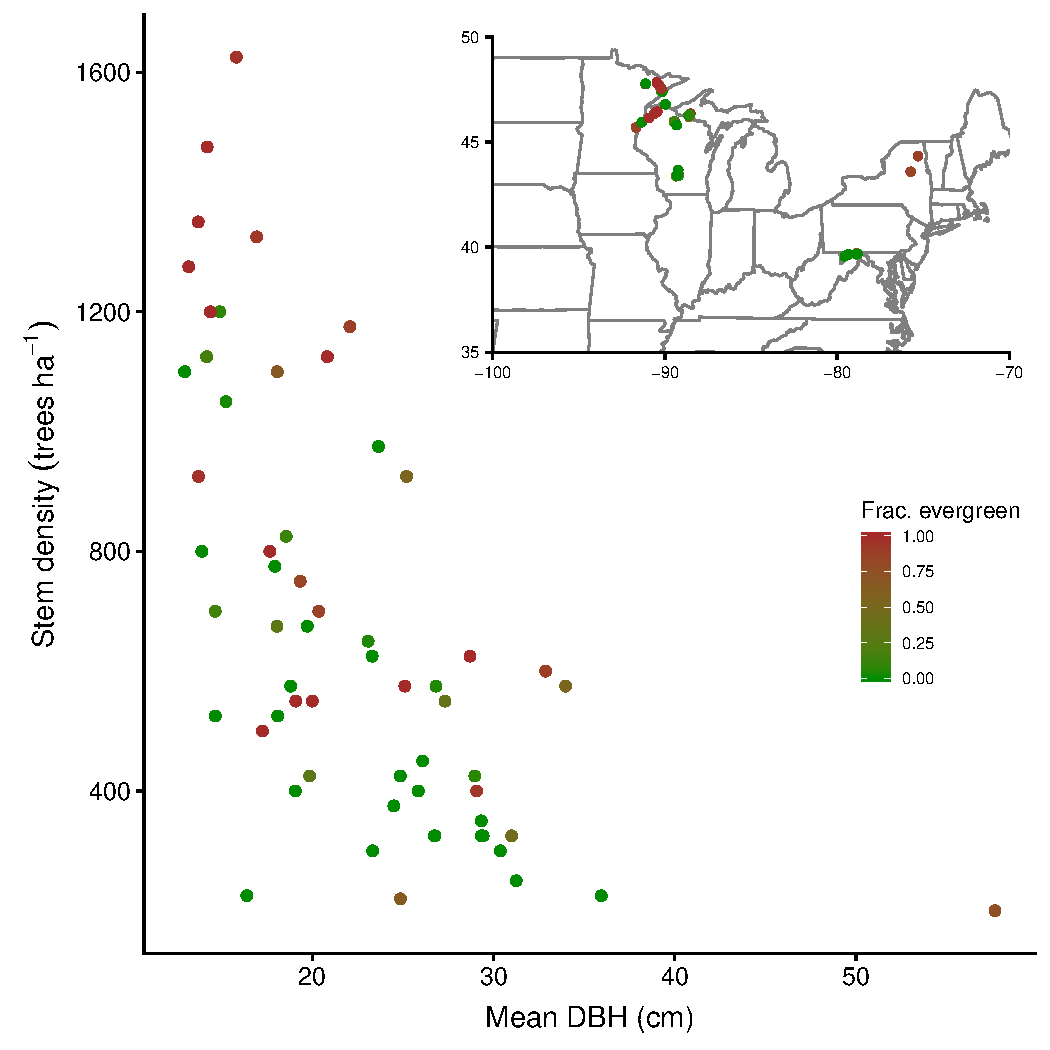
\includegraphics[width=\textwidth]{figures/sites_both.pdf}
  \caption{\
    Sites selected for analysis, in ``stand structure'' (\textit{main figure}) and geographic (\textit{inset}) space.
    Colors indicate the fraction of the stand that is made up of evergreen PFTs.
    Large points with labels indicate sites that were selected for forward simulations.
  }\label{fig:sites}
\end{figure}
% * <fer.istem@gmail.com> 2018-05-02T19:51:35.047Z:
% 
% not sure if it matters but the deciduousness gradient is not detectible from the color scheme, all points seem either 0 or 1 to me
% 
% ^.
% TODO: Change colors to be top cohort

I calibrated EDR using the same general Bayesian RTM inversion described in Chapter 3.
The inversion fit all sites simultaneously, such that at every MCMC iteration, the algorithm proposed a set of all parameter values for each PFT and simulated spectra for each site based on its observed composition and structure.
Because of unrealistic values in the shortwave infrared spectral region in the AVIRIS observations, likely caused by faulty atmospheric correction, I only calibrated the model with observations from 400 to 1300 nm.
% TODO: If I use it: Heteroskedastic variance model, fixed allometry parameter.
To generate the initial history state files required by EDR, I ran ED2 itself for one day in midsummer (July 1), starting from vegetation initial conditions based on observed composition and structure.

For priors on the five PROSPECT parameters and specific leaf area, I performed a hierarchical multivariate analysis (see Chapter 1) on PROSPECT parameters estimated from chapter 3 and, where available, direct measurements of specific leaf area. 
For priors on the leaf biomass allometry parameters, I fit a multivariate normal distribution using the \texttt{PEcAn.allometry} package (fit to its default data source). % TODO: More on this?
% * <dietze@bu.edu> 2018-05-02T22:07:34.089Z:
% 
% Default data source is Jenkins
% 
% ^.
For the clumping factor, I used a uniform prior across its full range (0 to 1), and for the leaf orientation factor, I used a weakly informative re-scaled beta distribution centered on 0.5.

I present posterior estimates for each parameter summarized as mean and 95\% confidence interval (Figure~\ref{fig:pda_posteriors}).
To evaluate the performance of the model, I compared the prior and posterior credible interval of the modeled spectra to the observations at each site (Figure~\ref{fig:sites}).
% * <dietze@bu.edu> 2018-05-02T22:08:48.140Z:
% 
% You shouldn't include links to analysis figures in the Methods section -- those should come in the Results
% 
% ^.
To assess any systematic errors in calibration, I also calculated the mean bias and root mean square error (RMSE) between the observed and mean predicted spectra binned across the visible (400--750 nm) and near infrared (750--1300 nm) spectral regions and plotted these values as a function of site mean DBH and stand density similarly to Figure~\ref{fig:sites} (Figure~\ref{fig:bias}).
As LAI in EDR is calculated from the parameters at each step, I also compared EDR estimates of LAI to observed values (Figure~\ref{fig:lai_validation}). %, and investigated the extent to which errors in predictions of spectra and LAI were related (Figure~\ref{fig:spec_lai}).

\subsection{Forward simulation}

I selected six sites for the ED2 forward simulation representative of the overall structure and composition space (Figure~\ref{fig:sites}). %TODO: Check this number. Drop SF03? Why don't I have it?
Based on timber harvest data from the US Forest Service, I determined that one of these sites---OF05---was the site of a clear cut in 1982, which allowed me to simulate multidecadal dynamics of forest regrowth at this site by starting ED from near-bare ground in 1983.
For the remaining sites, I performed shorter simulations starting from the earliest available survey data (2008 for XXX, 2009 for YYYY).
I started all runs on June 2 of their respective start years (because ED runs are unstable when initialized from a leaf-off state), and stopped all runs on December 31, 2017.
For meteorological drivers, I used the North American Regional Reanalysis~(NCEP 2005)\nocite{narr}, selected due to its high temporal (3 hour) and spatial (32 km) resolution, availability of all variables required by ED (such as temperature, precipitation, and downwelling short- and longwave radiation fluxes), and uninterrupted data availability across the simulation period (including up to one month before present).
For soil inputs---namely, soil horizon classes and depths at each site---I extracted data from the US Department of Agriculture Soil Survey Geographic Database (SSURGO) using the \texttt{FedData} R package.

For each site, I ran 50 ED2 ensemble members, sampling traits randomly from the joint posterior distributions estimated in the calibration step.
Because the full vegetation dynamics version of ED2 is not configured to take PROSPECT spectra as an input, I set the parameters for leaf reflectance and transmittance to PROSPECT simulations averaged over the visible and near-infrared regions.
When the ED2 simulations were finished, I ran EDR over the ED2 outputs, generating a daily time series of hyperspectral reflectance for each ensemble member and site.
I then convolved these spectra to the six Landsat spectral bands using their known spectral response functions (as in Chapter 2),
and compared the resulting spectral time series to observed Landsat time series for each site obtained using Google Earth Engine.
To better capture the variability in the spectral data, I calculated the normalized difference vegetation index (NDVI) and tasseled cap spectral transformations (brightness, greenness, wetness) and used these as the basis for comparison.

\section{Results}

\subsection{Model calibration}

\begin{figure}
  \centering
  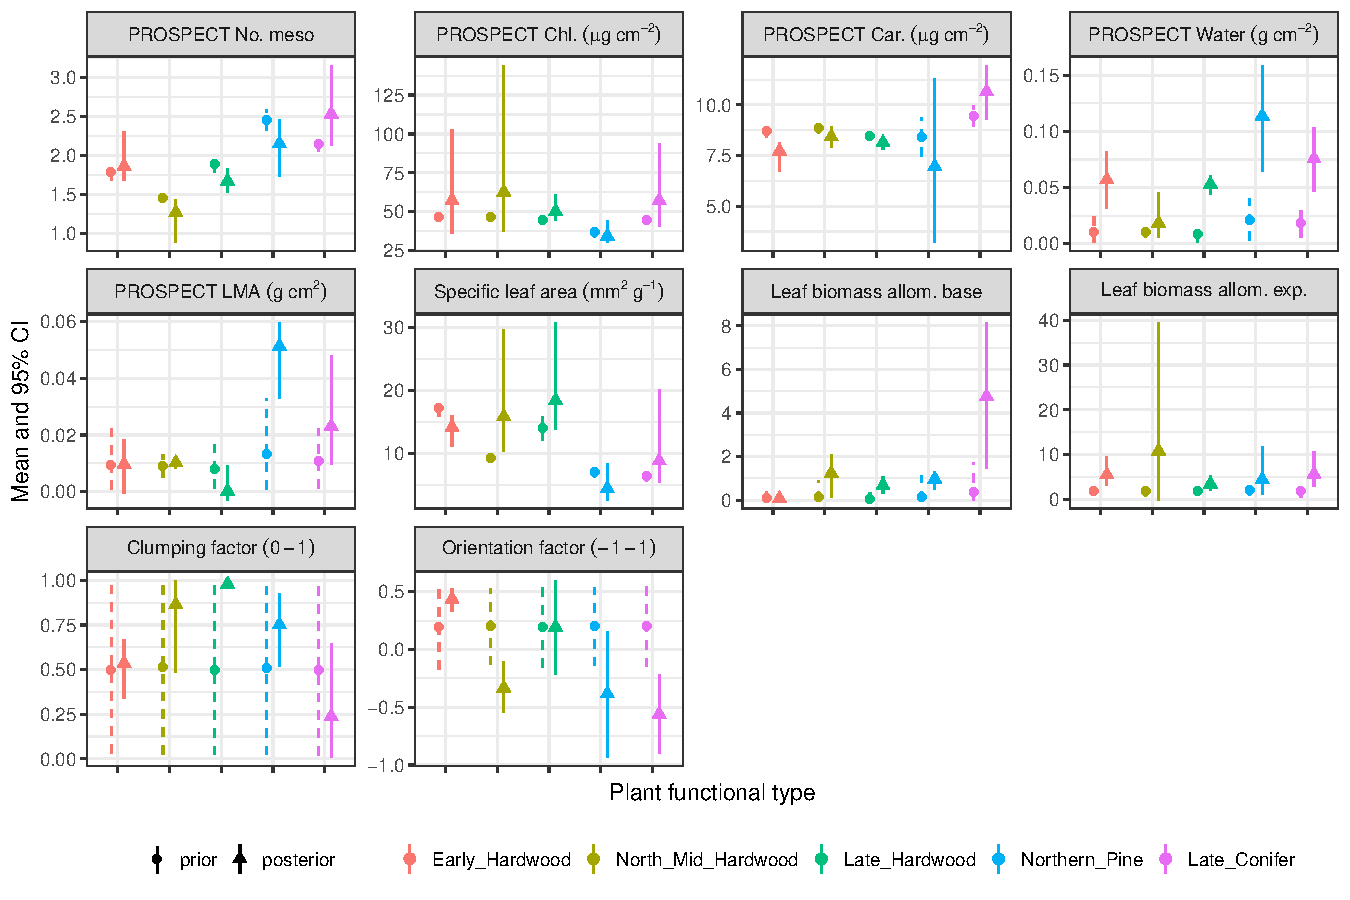
\includegraphics[width=\textwidth]{figures/pda_summary.pdf}
  \caption{\
    Summary statistics for model calibration parameter prior and posterior distributions.
  }\label{fig:pda_posteriors}
\end{figure}

Marginal posterior distributions on parameters with highly informative priors (PROSPECT parameters, SLA, and leaf allometries) generally had higher uncertainty than prior distributions.
However, the orientation factor and especially the clumping factor were somewhat more constrained relative to their priors.
Analyis of joint posterior distributions reveals very tight covariance between many parameters and across PFTs, which explains the much tighter spectral confidence intervals relative to the prior (see Supplementary Information).

\begin{figure}
  \centering
  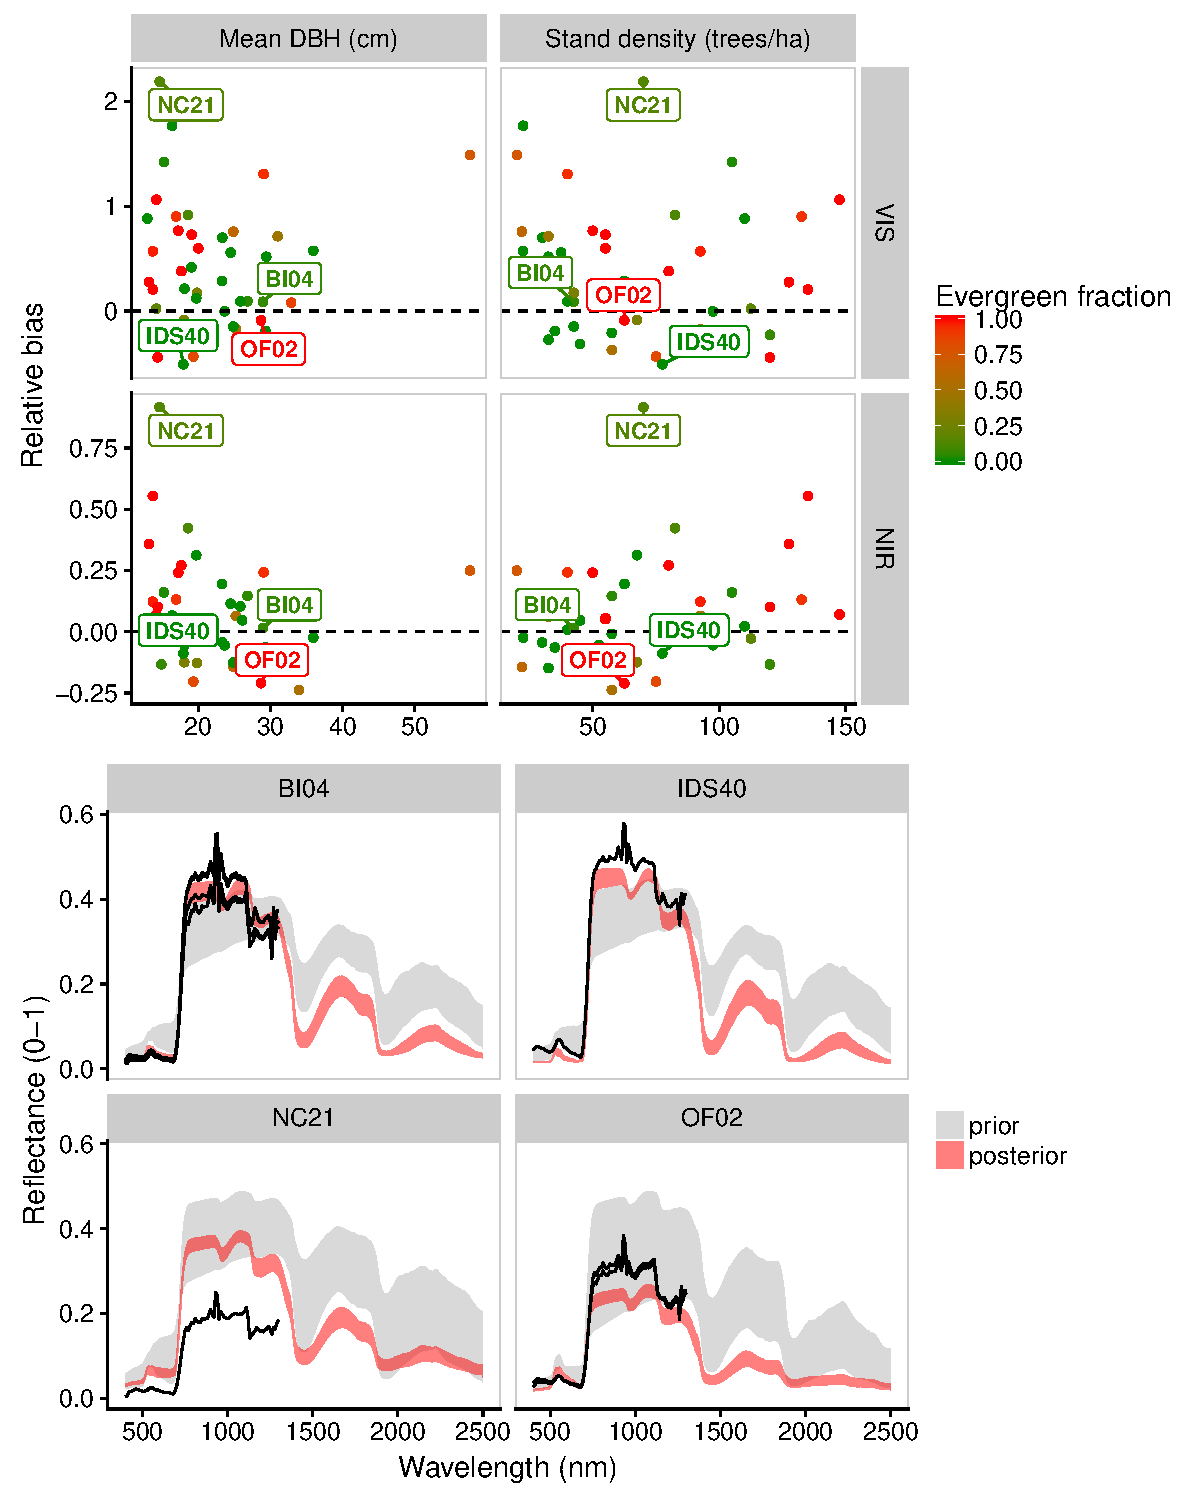
\includegraphics[width=\textwidth]{4_edr/figures/spec_validation.pdf}
  \caption{\
    (\textit{Top}) Relative bias of the posterior mean spectra at each site, aggregated across the visible (VIS, 400--750 nm) and near-infrared (NIR, 750--1300 nm) spectral range
    as a function of site mean diameter at breast height and stand density.
    (\textit{Bottom}) Prior and posterior predictive intervals and AVIRIS observations for four sites representative of different kinds of error.
  }\label{fig:bias}
\end{figure}

In general, after calibration across a large number of structurally and functionally diverse sites, EDR was able to reproduce observed AVIRIS canopy reflectance reasonably well.
However, performance was strongly site specific.
At many sites, but most prominently those composed of small trees (DBH < 20, e.g.\ site NC21), EDR frequently overestimated canopy reflectance.
That being said, least-squares linear regressions of relative spectral bias as a function of site mean DBH or stand density were not statistically significant ($p > 0.1$).
EDR was generally more likely to overestimate canopy reflectance for conifer trees than broadleaved trees.

\begin{figure}
  \centering
  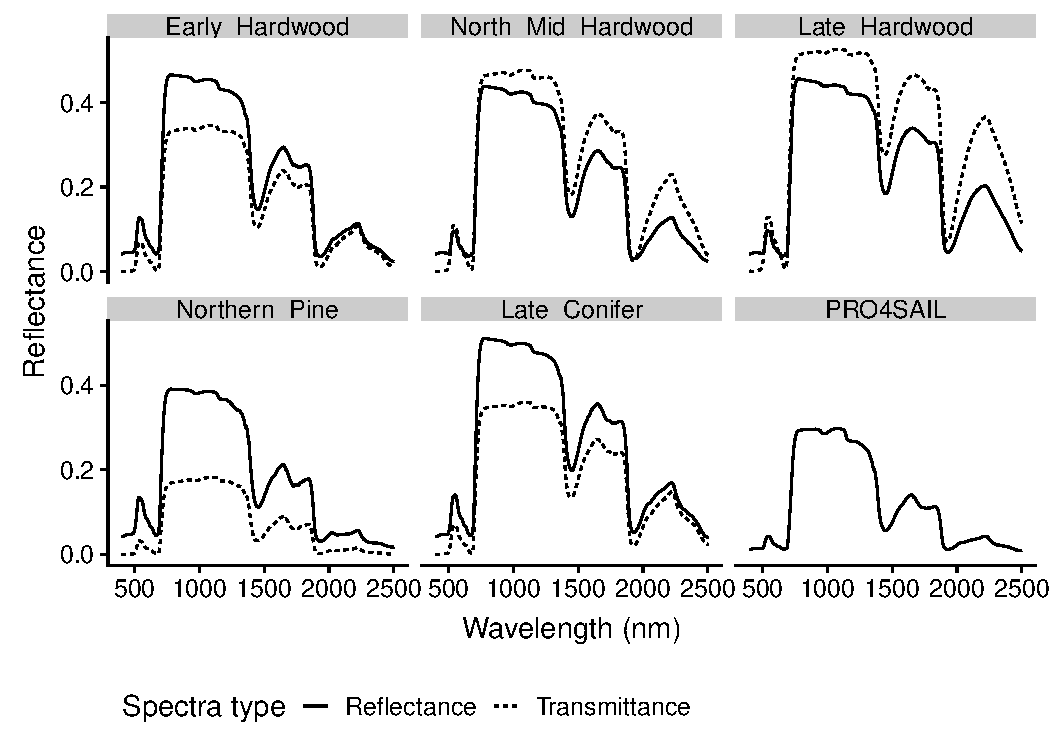
\includegraphics[width=\textwidth]{4_edr/figures/explore_spectra/pft_prospect_sim.pdf}
  \caption{%
    First five panels are PROSPECT simulations of leaf reflectance and transmittance for the plant functional types used in this analysis, based on parameters at their posterior means.
    The final panel is a simulation using the PRO4SAIL~\cite{verhoef_1984_sail} canopy radiative transfer model, parameterized with default structural parameters and leaf parameters averaged across the posterior means of the five plant functional types.
    % TODO: Add SAIL simulation
  }
\end{figure}

\begin{figure}
  \centering
  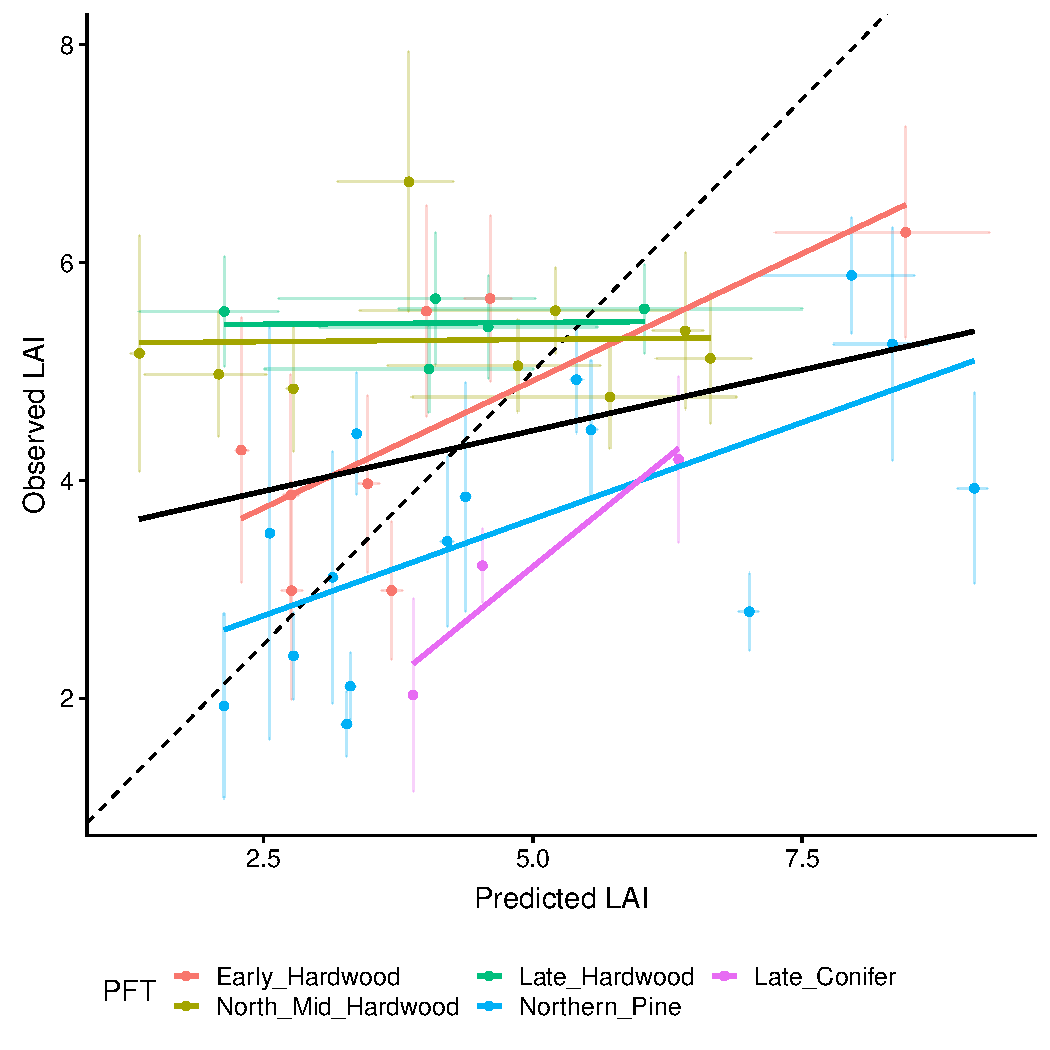
\includegraphics[width=\textwidth]{4_edr/figures/explore_spectra/lai_scatter.pdf}
  \caption{\
    Predictions of leaf area index by EDR, compared to observed values.
    Colors indicate the plant functional type of the tallest cohort at each site.
    % TODO: Add by-PFT regression line
  }\label{fig:lai_validation}
\end{figure}

\begin{figure}
  \centering
  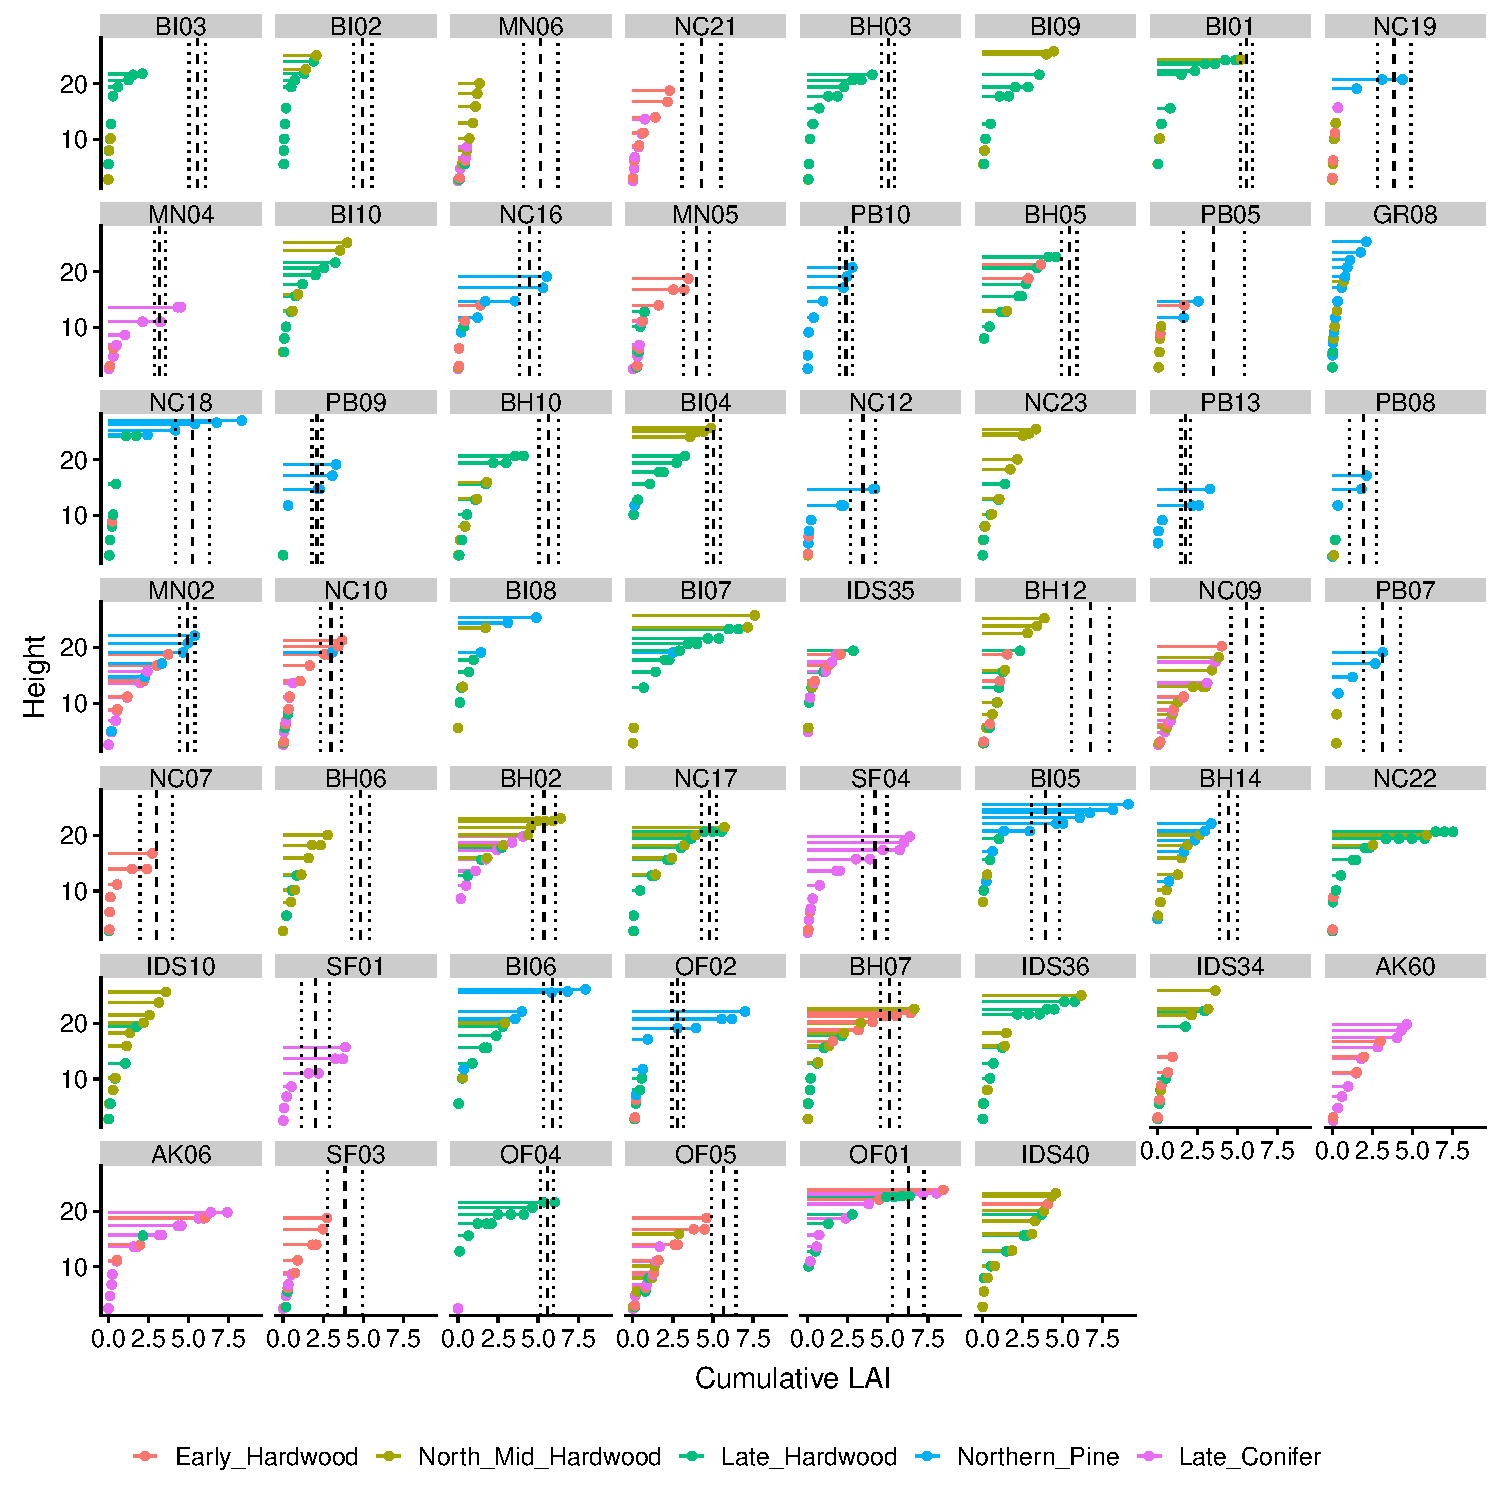
\includegraphics[width=\textwidth]{4_edr/figures/explore_spectra/ed_cumlai_plot.pdf}
  \caption{%
    Vertical profile of cumulative leaf area index and composition at each site in this analysis.
    Vertical black lines indicate the mean $\pm$ 1 standard deviation of the observed leaf area index.
  }
\end{figure}

EDR predictions of LAI also agreed reasonably well with observations for most sites.
EDR tended to overestimate LAI for conifer-dominated stands and slightly underestimate it for deciduous stands.

%\begin{figure}
  %\centering
  %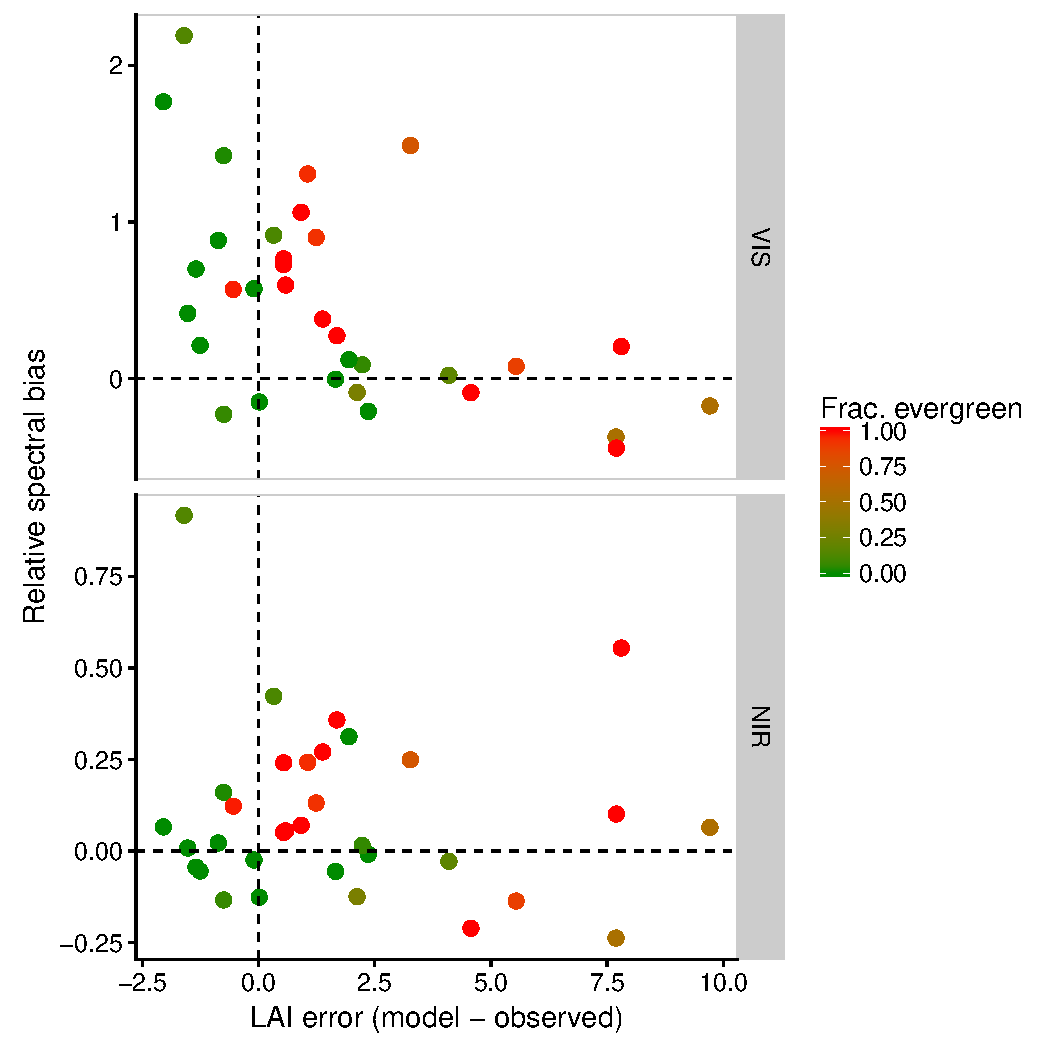
\includegraphics[width=\textwidth]{figures/spec_lai.pdf}
  %\caption{\
    %Relationship between errors in EDR predictions of leaf area index and spectra.
  %}\label{fig:spec_lai}
%\end{figure}

%There was a significant negative relationship between EDR LAI errors and spectral errors in the visible range;
%in other words, EDR tended to overestimate either LAI or canopy reflectance.

\subsection{Forward simulation}

\begin{figure}
  \centering
  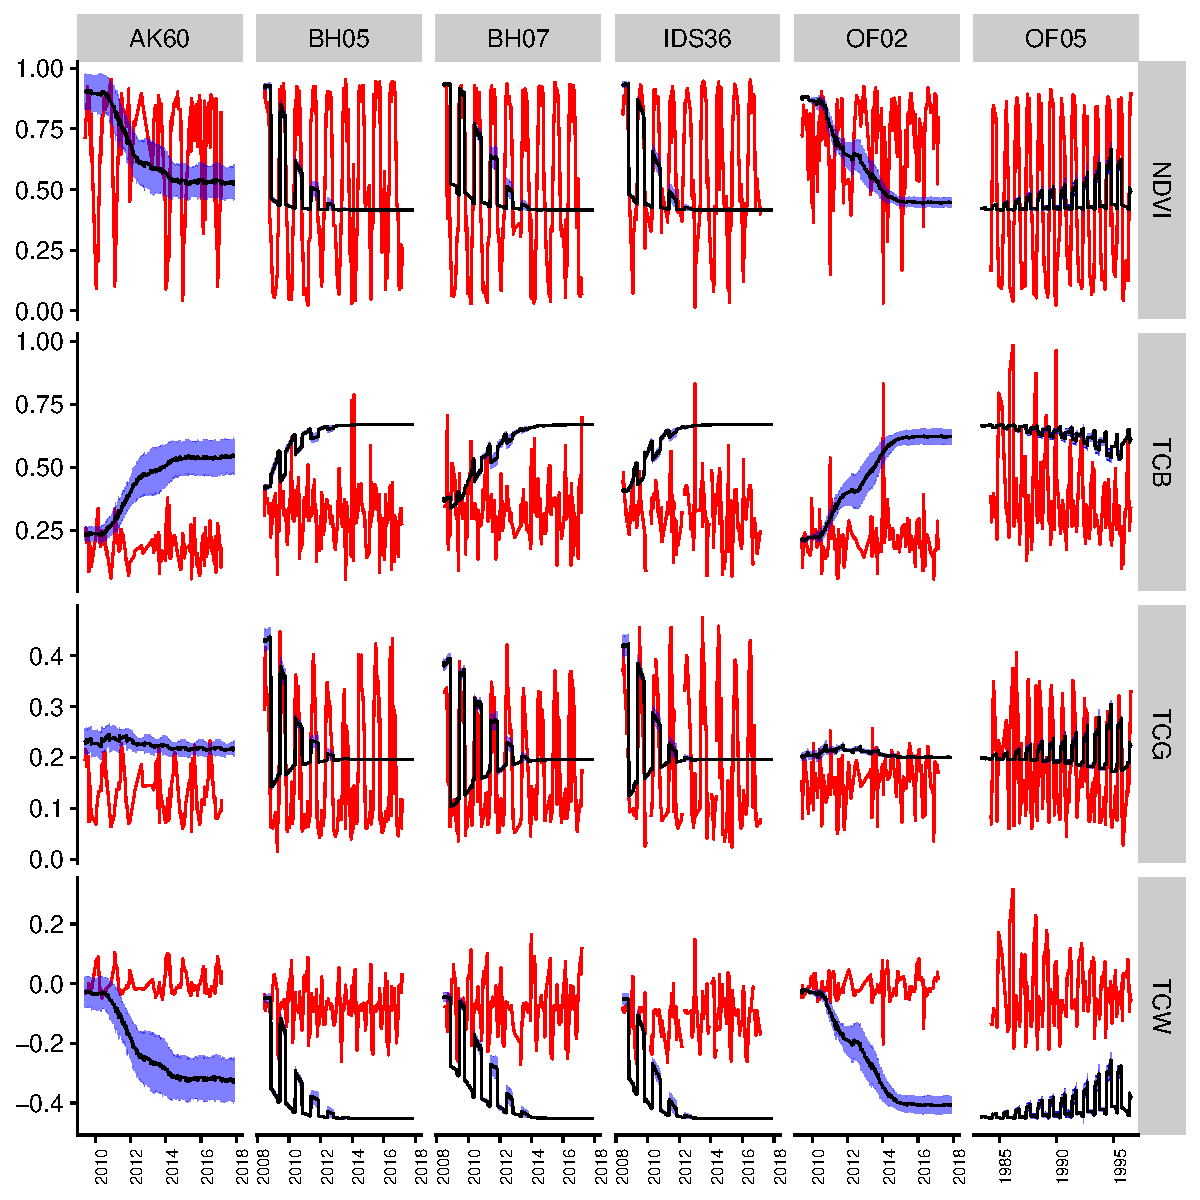
\includegraphics[width=\textwidth]{figures/landsat_ts.pdf}
  \caption{\
    Comparison of EDR-simulated (black, blue ribbon) and observed (red) time series of Landsat NDVI and tasseled cap brightness (TCB), greenness (TCG), and wetness (W) for each site.
  }
\end{figure}

(Currently working on this text\ldots).

\section{Discussion and conclusions}

The accurate simulation of canopy radiative transfer is key to a number of ecosystem processes, including photosynthesis, soil respiration, and hydrology.
However, to date, accurate parameterization of canopy radiative transfer in vegetation models has received relatively little attention compared to other canopy processes.
This study shows that remotely sensed surface reflectance can be used effectively to both parameterize and diagnose errors in radiative transfer models.

For its representation of radiative transfer, EDR uses the two-stream solutions of Sellers (1983) adapted for multiple canopies.
My results show that this scheme tends to systematically over-predict canopy-level reflectance in the visible spectral region (Figure~\ref{fig:spec_error_vis}), which may have important consequences for photosynthesis since it implies an under-prediction of the overall fraction of absorbed photosynthetically active radiation and therefore photosynthesis.
The predictions of EDR also appear to be systematically higher than those of a different two-stream radiative transfer model---SAIL~\cite{verhoef_1984_sail}---for roughly the same set of leaf reflectance parameters (Figures~\ref{fig:prospect_posterior}), which suggests that ED's representation of canopy structure and its effects on radiation are likely at fault.

I suggested in the results section that ED's systematic errors are driven by placing too much weight on leaf reflectance relative to transmittance.
This is supported by the low orientation factor estimates for late hardwoods and northern pines (Figure~\ref{fig:pda_posteriors}), since lowering the orientation factor is one way to place more weight on transmittance relative to reflectance (see model description in Methods).
Another way to reduce visible reflectance is to reduce leaf area index, which may be why predicted leaf area index for northern pine tends to be over-predicted.
The underlying reason for these issues may be that the naive multi-layer structure of ED, combined with the Sellers (1983) two-stream equations, means that the effect of leaf transmittance declines much faster than the effect of reflectance, and places very high weight on reflectance from the top canopy layer (because the contribution of lower layers declines exponentially).
Future work will attempt to diagnose these issues in more detail, and to investigate the extent to which these same issues are pervasive in other common representations of radiative transfer found in other models. 

\subsection{Future directions}

Finite crown model, following Dietze and Clark (2008)\nocite{}

Improved simulations of snow and soil reflectance.
Soil reflectance can be modeled as a function of soil moisture following the Hapke model\cite{HAPKE}.
Snow reflectance can be modeled based on snow water equivalent\cite{SWE}.

Simulating remote sensing time series and comparing to observations.
A promising new way to validate ecosystem dynamics.


%\section{Conclusions}

The objective of this study was to calibrate the canopy radiative transfer model inside of the ED2 dynamic demographic vegetation model by comparing its predictions of surface reflectance against direct observations thereof by airborne imaging spectroscopy.
In general, the calibration successfully constrained the posterior distributions of model parameters related to canopy structure (leaf angle, canopy clumping, and leaf area index) for five plant functional types characteristic of temperate forests of the northeastern United States.  
However, comparisons of predicted spectra post-calibration against observations reveal widespread biases, which indicates that there are structural issues with the ED2 radiative transfer model that inhibit its ability to accurately predict surface optical properties.
Sensitivity analyses, along with comparison against an alternative canopy radiative transfer model more commonly used by the remote sensing community (4SAIL), shed additional light on the problem and provides avenues for future exploration and model improvement.
One issue was unrealistically high sensitivity to wood reflectance, which contributed to a positive bias.
Future work could add parameters related to wood to the calibration step, and consider alternative representations of wood reflectance.
This is low-hanging fruit and should be the first refinement to this analysis.
However, wood reflectance alone was insufficient to explain the positive bias in ED2 compared to 4SAIL.
Another source of error suggested in the discussion was excessive sensitivity to soil reflectance.
Future investigation should compare the sensitivities of EDR and 4SAIL to soil reflectance, particularly under dense, closed canopies, to determine whether there is in fact excessive sensitivity.
Even if the sensitivity is correct, this study's use of a fixed soil background likely contributed significant errors for the many sites with young, open canopies and exposed understories, and future work would do well to incorporate soil variability to some extent to the calibration.
Finally, potential utility of doing all this with time series...


\cleardoublepage

% -------------------------------------
% CHAPTER 3: CONCLUSION
% -------------------------------------
%\chapter{Conclusions}
\label{chapter:Conclusions}
\thispagestyle{myheadings}

% set this to the location of the figures for this chapter. it may
% also want to be ../Figures/2_Body/ or something. make sure that
% it has a trailing directory separator (i.e., '/')!
\graphicspath{{3_Conclusion/Figures/}}

\section{Summary of the thesis}

Time to get philosophical and wordy.

IMPORTANT: In the references at the end of thesis, all journal names must be
spelled out in full, except for standard abbreviations like IEEE, ACM, SPIE,
INFOCOM, ...
%\cleardoublepage

%\appendix
\begin{appendices}
\chapter{Proof of xyz}
\label{appendix}
\thispagestyle{myheadings}

This is the appendix.
\end{appendices}
%==========================================================================%
% Bibliography
\newpage
\singlespace
\bibliographystyle{apalike}

% each subdirectory can have its own BiBTeX file
\bibliography{library}
\cleardoublepage

%==========================================================================%
% Curriculum Vitae
\addcontentsline{toc}{chapter}{Curriculum Vitae}

\thispagestyle{empty}

\begin{center}
{\LARGE {\bf CURRICULUM VITAE}}\\
\vspace{0.5in}
{\large {\bf Alexey N Shiklomanov}}
\end{center}

\section*{Education}

\begin{itemize}
  \item Ph.D. Geography, Boston University (Exp. June 2018)
  \item Honors B.S. with Distinction, Chemistry \& Environmental Science, University of Delaware (May 2014)
    \begin{itemize}
      \item \textit{Magna cum laude}
      \item Geography minor
      \item Honors thesis: \textit{Stemflow acid neutralization capacity in a deciduous forest: the role of edge effects.} Advisor: Delphis Levia
    \end{itemize}
\end{itemize}

\section*{Publications}

\subsection*{Published}

\begin{itemize}
  \item 2017.~Kaverin, D.A.; Melnichuk, E.B.; Shiklomanov, N.I.; Kakunov, N.B.; Pastukhov, A.V.; \textbf{Shiklomanov, A.N.}.
    Long-term changes in the ground thermal regime of an artificially-drained thaw lake basin: A case study in the Russian European North.
    \textit{Permafrost and Periglacial Processes}. \textbf{29}(1):49--59.

  \item 2016.~\textbf{Shiklomanov, A.N.}; Dietze, M.C.; Viskari, T.; Townsend, P.A.; Serbin, S.P. 
    Quantifying the influences of spectral resolution on uncertainty in leaf trait estimates through a Bayesian approach to RTM inversion. 
    \textit{Remote Sensing of Environment} \textbf{183}:226--238. 

  \item 2015.~Levia, D.F.; \textbf{Shiklomanov, A.N.}; Van Stan, J.T.; Sheick, C.E.; Inamdar, S.P.; Mitchell, M.J.; McHale, P.J. 
    Calcium and aluminum cycling in a temperate broadleaved deciduous forest of the eastern USA\@: relative impacts of tree species, canopy state, and flux type. 
    \textit{Environmental Monitoring and Assessment} \textbf{187}(7):4675. 

  \item 2014.~\textbf{Shiklomanov, A.N.} \& Levia, D.F. 
    Stemflow acid neutralization capacity in a broadleaved deciduous forest: The role of edge effects. 
    \textit{Environmental Pollution} \textbf{193}:45--53. 
\end{itemize}

\subsection*{In review}

\begin{itemize}
  \item \textbf{Shiklomanov, A.N.}; Cowdery, E.M.; Bahn, M.; Byun, C.; Craine, J.; Gonzalez-Melo, A.; Jansen, S.; Kraft, N.; Kramer, K.; Minden, V.; Niinemets, Ü.; Onoda, Y.; Sosinski, E.; Soudzilovskaia, N.; Dietze, M.C. 
    Does the leaf economic spectrum hold within plant functional types? A Bayesian multivariate trait meta-analysis.
    \textit{New Phytologist}.

  \item \textbf{Shiklomanov, A.N.}; Smallman, L.; Bradley, B.; Dahlin, K.; Fox, A.; Gough, C.; Hoffman, F.M.; Middleton, E.; Serbin, S.; Smith, W. The role of remote sensing in global change experiments. \textit{Frontiers in Ecology \& Evolution}.

  \item Viskari, T.; \textbf{Shiklomanov, A.N}.; Dietze, M.C.; Serbin, S.P. The influence of canopy radiation parameter uncertainty on model projections of carbon and energy cycling.
    \textit{Journal of Advances in Modeling Earth Systems}.
\end{itemize}

\section*{Conference \& Workshop Presentations}

\subsection*{Invited}

\begin{itemize}
  \item Ecological Society of America (ESA) Annual Meeting.
  Invited ignite presentation: ``Applications of radiative transfer modeling to vegetation remote sensing''.
  August 2017

  \item American Geophysical Union (AGU) Fall Meeting.
  Invited oral presentation: ``Leaf optical properties shed light on foliar trait variability at individual to global scales''.
  December 2016.
\end{itemize}

\subsection*{Contributed}

\begin{itemize}
  \item NASA Biodiversity \& Ecological Forecasting Team Meeting
    Poster presentation: ``Cutting out the middle man: Calibrating and validating an ecosystem model with remotely sensed surface reflectance''.
    April 2018.

  \item American Geophysical Union (AGU) Fall Meeting.
    Oral presentation: ``Leaf optical properties shed light on foliar trait variability at individual to global scales''.
    December 2017.

  \item 39th New Phytologist Symposium --- Trait covariation: Structural and functional relationships in plant ecology.
    Poster presentation: ``Leaf optical properties shed light on foliar trait variability at individual to global scales''.
    June 2017.

  \item NASA Biodiversity \& Ecological Forecasting Team Meeting
    Poster presentation: ``Leaf optical properties shed light on foliar trait variability at individual to global scales''.
    May 2017.

  \item American Association of Geographers (AAG) Fall Meeting.
    Oral presentation: ``Leaf optical properties shed light on foliar trait variability at individual to global scales''.
    April 2017.

  \item American Geophysical Union (AGU) Fall Meeting.
    Oral presentation: ``Scaling and breaking the leaf economic spectrum: Leaf trait relationships diverge across plant functional types''.
    December 2016.

  \item American Geophysical Union (AGU) Fall Meeting. 
    Poster presentation: ``Applications of spectral inversion to understanding vegetation functional trait relationships.''
    December 2015.

  \item NASA Carbon Cycle \& Ecosystems Conference. 
    Poster presentation: ``Chloroplasts to canopies: Analysis of leaf spectral trait variability across spatial scales.'' 
    April 2015.

  \item North American Carbon Program (NACP) Fall Meeting. 
    Poster presentation: ``Characterization of uncertainties in leaf traits through a Bayesian inversion of the PROSPECT model.'' 
    January 2015.
\end{itemize}


\section*{Workshop and working group participation}

\begin{itemize}
  \item USGS Biodiversity and Climate Modeling Workshop Series.
    June 2017, March 2018.

  \item Oak Ridge National Lab Data Distributed Active Archive Center (DAAC) User Working Group (UWG) meeting. 
    May 2017.

  \item INTERFACE Workshop on Frontiers in terrestrial climate feedbacks: Integrating models and experiments to explore climate feedbacks in a managed and warming world. 
    February 2016.

  \item Keck Institute for Space Sciences (KISS) Workshop: Exploring New Multi-Instrument Approaches to Observing Terrestrial Ecosystems and the Carbon Cycle from Space.  
    October 2015.
\end{itemize}


\section*{Teaching experience}

Certified Software Carpentry instructor. Taught the following workshops:
\begin{itemize}
  \item R, Unix Shell, Git --- Federal Reserve Board (August 2017)
  \item Python, Unix Shell, Git, SQL --- University of West Virginia (May 2017)
  \item Python, Unix Shell, Git --- University of California-San Francisco Medical School (December 2016)
\end{itemize}

\section*{Research Grants}

\begin{itemize}
  \item Spring 2016: NASA Earth \& Space Science Fellowship: ``Tracking successional dynamics of foliar traits using remote sensing'', \$30,000
  \item Spring 2015: Boston University Biogeoscience Student Award, \$500
  \item Winter 2014: Senior Thesis Winter Session Scholars Award, \$600
  \item Summer 2013: Delaware Water Resources Center (DWRC) summer research grant: ``Acid neutralization in a deciduous forest: The role of edge effects'', \$3500
  \item Spring 2013: University of Delaware undergraduate research program supply and expense grant, \$700
\end{itemize}


\section*{Awards and Recognition}

\begin{itemize}
  \item Honorable Mention, National Science Foundation Graduate Research Fellowship Program (GRFP), (Spring 2016)
  \item Honorable Mention, National Science Foundation Graduate Research Fellowship Program (GRFP), (Spring 2015)
  \item Outstanding Senior in Environmental Science, University of Delaware (Spring 2014)
  \item Phi Beta Kappa, Alpha of Delaware Chapter (Spring 2014)
  \item Special Merit Award for Outstanding Achievement in Environmental Science, University of Delaware (Spring 2013)
  \item University of Delaware Dean's List (Fall 2010--Spring 2014)
  \item University of Delaware Governor's Scholarship (Spring 2011--Spring 2014)
  \item University of Delaware Scholar --- merit scholarship (Spring 2010--Spring 2014)
\end{itemize}

%%% Local Variables:
%%% mode: latex
%%% TeX-master: "../dissertation"
%%% End:
 

%==========================================================================%
\end{document}
